%%%% DOCUMENT CLASS ************************************************************
%\documentclass[print,thumbmain]{src/thesis}  % uncomment for writing
\documentclass[final]{src/thesis} % uncomment for rendering/final version

%%%% PREAMBLE ******************************************************************
%!TEX root = ../thesis.tex
%\usepackage{amsmath}
\usepackage[fleqn]{amsmath}
\usepackage{amsfonts}
\usepackage{amssymb}
\usepackage{accents}
\usepackage{amsthm}
\usepackage{appendix}
\usepackage{afterpage}
\usepackage{array}
\usepackage[dutch,english]{babel}
\usepackage[autostyle]{csquotes}
\usepackage{enumitem}
\usepackage{epsfig}
\usepackage{epstopdf}
\usepackage{fancyhdr}
\usepackage{float}
\usepackage{graphicx}
\usepackage{lipsum}
\usepackage{longtable}
\usepackage{multicol}
\usepackage{multirow}
\usepackage[numbers,sort&compress]{natbib}
\usepackage[final]{pdfpages}
\usepackage{relsize}
\usepackage{subfig}
\usepackage{siunitx}

\usepackage{tcolorbox}
\usepackage{thmtools}
\usepackage{todonotes}
%\usepackage{tikz}      % The tikz package is added in mrthesis.cls for producing thumbindex
\usepackage{url}
\usepackage{xcolor}
\usepackage{textcomp}

\usepackage[bookmarks=true,bookmarksopen=false,colorlinks=true,pdfpagelayout=TwoColumnRight]{hyperref}
\hypersetup{
    colorlinks,%
    citecolor=black,%
    colorlinks=true,%
    filecolor=black,%
    linkcolor=black,%
    urlcolor=gray,
    }
\usepackage{bookmark}

\setlength{\mathindent}{1.75cm}

%!TEX root = ../thesis.tex

% Texts or
\newcommand{\ie}{\textit{i.e.}}
\newcommand{\eg}{\textit{e.g.}}
\newcommand{\blank}{\,\cdot\,}
\renewcommand{\emph}[1]{'\textit{#1}'}
\newcommand{\sorotoki}{\textup{\texttt{SOROTOKI}} }
\newcommand{\matlab}{\textup{\texttt{MATLAB}} }
\newcommand{\data}[1]{(\raisebox{-2.7pt}{\textcolor{#1}{\,\Huge{\textbf{-}}}})}
\newcommand{\ldata}[1]{\raisebox{-2.7pt}{\textcolor{#1}{\,\Huge{\textbf{-}}}}}

% Equations/math
\newcommand{\be}{\begin{equation}}
\newcommand{\ee}{\end{equation}}
\newcommand{\benn}{\begin{equation*}}
\newcommand{\eenn}{\end{equation*}}
\newcommand{\bea}{\begin{eqnarray}}
\newcommand{\eea}{\end{eqnarray}}
\newcommand{\beann}{\begin{eqnarray*}}
\newcommand{\eeann}{\end{eqnarray*}}
\newcommand{\ba}{\begin{align}}
\newcommand{\ea}{\end{align}}
\newcommand{\bpm}{\begin{pmatrix}}
\newcommand{\epm}{\end{pmatrix}}
\newcommand{\bbm}{\begin{bmatrix}}
\newcommand{\ebm}{\end{bmatrix}}
\newcommand{\bc}{\begin{center}}
\newcommand{\ec}{\end{center}}
\newcommand{\pwr}[1]{\cdot10^{\textrm{#1}}}

% Symbols and annotations
%\newcommand{\fB}{\boldsymbol{f}}
\newcommand{\maT}{\text{ma}}
\newcommand{\qR}{\mathrm{q}}
\newcommand{\RBB}{\mathbb{R}}
\newcommand{\rmsT}{\text{rms}}
\newcommand{\xBF}{\mathbf{x}}
\newcommand{\interior}{\operatorname{int}}

% Tikz figures
\newcommand{\SF}{1}                 % Scaling factor
\newcommand{\TS}{\normalsize}       % Text size
\newcommand{\lw}{0.7pt}             % Line width
\newcommand{\TSTick}{\small}        % Text size axis labels
\newcommand{\axislabels}[2]{\foreach \x/\y/\s in {#1} {\node[#2,inner sep=1mm] at (\x,\y) {\TSTick $\s$};}}
\newcommand{\wheel}[3]{ \draw[line width=\lw] (#1,#2) circle (#3);
                        \fill[bottom color=MRblue!60!black!80,top color=MRblue!10] (#1,#2) circle (#3-0.5*\lw);
                        \fill[color=MRblue!30] (#1,#2) circle (#3-\lw);
                        \fill[top color=MRblue!60!black!80,bottom color=MRblue!10] (#1,#2) circle (0.7*#3);
                        \fill[color=MRblue!30] (#1,#2) circle (0.7*#3-\lw);
                        \fill[color=black] (#1,#2) circle (0.1*#3);}

\newcommand{\CoM}[3]{\filldraw[inner color=white,outer color=black!7!white,draw=black,line width=\lw] (#1,#2) circle (#3+0.5*\lw);
                     \begin{scope}[xshift=#1,yshift=#2]
                        \clip(-#3,0) -- (0,0) -- (0,#3) -- (#3,#3) -- (#3,0) -- (0,0) -- (0,-#3) -- (-#3,-#3) -- cycle;
                        \fill[inner color=black!50!white,outer color=black] (0,0) circle (#3);
                     \end{scope}}

\definecolor{MRdarkblue}{RGB}{16,9,88}      % Define a set of colors to be used throughout thesis
\definecolor{MRred}{RGB}{152,0,0}
\definecolor{MRgreen}{RGB}{0,146,69}
\definecolor{MRblue}{RGB}{53,153,204}
\definecolor{MRorange}{RGB}{220,85,30}
\definecolor{MRlightgreen}{RGB}{217,224,33}
\definecolor{MRyellow}{RGB}{255,214,0}
\definecolor{MRgrey}{gray}{0.95}
\usetikzlibrary{arrows}
\usetikzlibrary{patterns}
\usetikzlibrary{decorations.markings}
\usetikzlibrary{shadings}
\usetikzlibrary{shapes}

% Counters
\newcounter{ContNum}        % Counter for the contributions
\renewcommand{\theContNum}{\Roman{ContNum}}

% Other
\newcommand\blankfootnote[1]{%
  \let\thefootnote\relax\footnotetext{#1}%
  \let\thefootnote\svthefootnote%
}
\newcounter{numfootnote}
\newcommand\numfootnote[1]{%
    \stepcounter{numfootnote}%
    \newcommand{\thefootnote}{\thenumfootnote}%
    \footnote{#1}
}

\newcommand{\disclaimer}{\\[\baselineskip]  A detailed list of the differences between this chapter and the article on which it is based is provided in the %\hyperref[chap: Modifications]{\emph{Modifications}}
\emph{Modifications} chapter of this thesis.}
\newcommand{\itemheader}[1]{~\\ \noindent\textbf{#1.}\ \ }
\newcommand{\itemheaderNewpage}[1]{\newpage \noindent\textbf{#1.}\ \ }
\newcommand{\contribution}[2]{\refstepcounter{ContNum}#2 \vspace*{2.1mm}\begin{tcolorbox}[colback=black!2!white,colframe=black!20!white] \textbf{Contribution \Roman{ContNum}.} {\em #1} \end{tcolorbox}\vspace*{2.1mm}}
\newcommand{\objective}[1]{\begin{tcolorbox}[colback=black!2!white,colframe=black!20!white] {\em #1} \end{tcolorbox}}
\newcommand{\terminology}[2]{\begin{tcolorbox}[colback=black!2!white,colframe=black!20!white] {\textbf{Terminology: } \textbf{#1} \em #2} \end{tcolorbox}}
\newcommand{\cover}[1]{\ifprint{}\else\includepdf[pages=-]{#1}\cleardoublepage\fi}

\newcommand\tcircle[1]{%
  \raisebox{-0.25pt}{%
    \textcircled{\fontsize{8pt}{0}\selectfont #1}%
  }%
}

\newenvironment{Nomen}
    {\vspace*{-3mm}\begin{center}
    \begin{longtable}{p{.1\textwidth} p{.93\textwidth}}
    }
    {
    \end{longtable}
    \end{center}\vspace*{-1.2cm}
    }

\newcommand{\AddSymbol}[2]{#1 & #2 \\}
%!TEX root = ../thesis.tex
%%%% ***************************************************************************
%%%% NOMENCLATURE **************************************************************
\usepackage{mathtools}

%%%%%%% ENTITIES %%%%%%%
\newcommand{\defas}[1]{\triangleq}
\newcommand{\grad}[1]{\nabla_{\!#1}\,}
\newcommand{\nn}{{n\times n}}

\newcommand{\ie}{\textit{i.e.}}
\newcommand{\eg}{\textit{e.g.}}
\newcommand{\blank}{\,\cdot\,}

% sets
\newcommand{\R}{\mathbb{R}}
\newcommand{\E}{\mathbb{E}}
\newcommand{\N}{\mathbb{N}}
\newcommand{\Z}{\mathbb{Z}}
\newcommand{\seg}[1]{\textup{\textrm{se}}(#1)}
\newcommand{\cose}[1]{\textup{\textrm{se}}^*(#1)}
\newcommand{\sog}[1]{\textup{\textrm{so}}(#1)}
\newcommand{\coso}[1]{\textup{\textrm{so}}^*(#1)}
\newcommand{\SO}[1]{\textup{\textrm{SO}}(#1)}
\newcommand{\SE}[1]{\textup{\textrm{SE}}(#1)}
\newcommand{\Sim}[1]{\textup{\textrm{Sim}(#1)}}
\newcommand{\atantwo}{\textup{\textrm{atan2}}}
\newcommand{\erf}{\textup{\textrm{erf}}}
\newcommand{\Id}{\text{id}}

% compact sets
\newcommand{\Rp}{\mathbb{R}_{\ge0}}
\newcommand{\Rn}{\mathbb{R}_{\le0}}
\newcommand{\Rsp}{\mathbb{R}_{>0}}
\newcommand{\Rsn}{\mathbb{R}_{<0}}
% domains
\newcommand{\Ts}{\mathbb{T}}
\newcommand{\Xs}{\mathbb{X}}
\newcommand{\Bs}{\mathbb{B}}
\newcommand{\Vs}{\mathbb{V}}
\newcommand{\Ss}{\mathbb{S}}
% functional
\newcommand{\Hm}{\mathcal{H}}
\newcommand{\La}{\mathcal{L}}
% tensors
\newcommand{\Mt}{\mathcal{M}}
\newcommand{\Ct}{\mathcal{C}}
\newcommand{\Ft}{\mathcal{F}}
\newcommand{\Uf}{\mathcal{U}}
\newcommand{\Wf}{\mathcal{W}}
\newcommand{\g}{\mathfrak{g}}
\newcommand{\Vf}{\mathcal{V}}
\newcommand{\Tf}{\mathcal{T}}
\newcommand{\Kf}{\mathcal{K}}
\newcommand{\Lf}{\mathcal{L}}

\newcommand{\p}{\partial}
\newcommand{\dt}{\Delta t}

\renewcommand{\d}{^{\raisebox{.2ex}{$\scriptscriptstyle d$}}}
\newcommand{\T}{^{\raisebox{.2ex}{$\scriptscriptstyle\top$}}}
\newcommand{\inv}{^{\raisebox{.2ex}{$\scriptscriptstyle-1$}}}
\newcommand{\pinv}{^{\raisebox{.2ex}{$\scriptscriptstyle\dagger$}}}
\newcommand{\ginv}{^{\raisebox{.2ex}{$\scriptscriptstyle+$}}}
\newcommand{\pinvt}{^{\raisebox{.2ex}{$\scriptscriptstyle+\top$}}}
%\newcommand{\grav}{^{\raisebox{.1ex}{$\scriptstyle\textrm{g}$}}}
%\newcommand{\elastic}{^{\raisebox{.1ex}{$\scriptstyle\textrm{e}$}}}
\newcommand{\grav}{_{\scriptstyle\textrm{g}}}
\newcommand{\elastic}{_{\scriptstyle\textrm{e}}}

\DeclarePairedDelimiter\ceil{\lceil}{\rceil}
\DeclarePairedDelimiter\floor{\lfloor}{\rfloor}

\renewcommand{\dim}{\text{dim}}
\newcommand{\trace}{\text{trace}}
\newcommand{\diag}[1]{\textnormal{diag}\left\{ {#1} \right\}}
\newcommand{\blkdiag}[1]{\textnormal{blkdiag}\left\{ {#1} \right\}}

\newcommand{\Q}{\mathcal{Q}}
\newcommand{\Qnc}{\vec{Q}^{\textrm{nc}}}
\newcommand{\q}{{\vec{q}}}
\newcommand{\dq}{{\dot{\vec{q}}}}
\newcommand{\ddq}{{\ddot{\vec{q}}}}
%\newcommand{\pB}{{\boldsymbol{\gamma}}}
\newcommand{\dpB}{{\dot{\boldsymbol{\gamma}}}}
\newcommand{\ddpB}{{\ddot{\boldsymbol{\gamma}}}}

%\newcommand{\MB}{\boldsymbol{M}}
%\newcommand{\CB}{\boldsymbol{C}}
%\newcommand{\NB}{\boldsymbol{N}}
%\newcommand{\GB}{\boldsymbol{G}}
%\renewcommand{\fB}{\boldsymbol{f}}
%\newcommand{\JB}{\boldsymbol{J}}
\newcommand{\dJB}{\dot{\boldsymbol{J}}}

\newcommand{\ad}{\textbf{ad}}
\newcommand{\Ad}{\textbf{Ad}}
\newcommand{\rank}{\textnormal{rank}}
\newcommand{\col}{\textnormal{col}}
\newcommand{\row}{\textnormal{row}}
\newcommand{\nc}{\textnormal{nc}}

%\newcommand{\gB}{\boldsymbol{g}}
%\newcommand{\UB}{\boldsymbol{U}}
%\newcommand{\LambdaB}{\boldsymbol{\Lambda}}
%\newcommand{\GammaB}{\boldsymbol{\Gamma}}
%\newcommand{\gammaB}{\boldsymbol{\gamma}}
%\newcommand{\KappaB}{\boldsymbol{\Kappa}}
%\newcommand{\phiB}{\boldsymbol{\phi}}
%\newcommand{\sB}{\boldsymbol{\sigma}}
%\renewcommand{\pB}{\boldsymbol{p}}
%\newcommand{\dB}{\boldsymbol{d}}
\newcommand{\ddB}{\dot{\boldsymbol{d}}}
%\newcommand{\FB}{\boldsymbol{F}}
\newcommand{\dFB}{\dot{\boldsymbol{F}}}
%\newcommand{\xB}{\boldsymbol{x}}
\newcommand{\dxB}{\dot{\boldsymbol{x}}}
\newcommand{\ddxB}{\ddot{\boldsymbol{x}}}
%\newcommand{\nuB}{\boldsymbol{\nu}}
%\newcommand{\JB}{\boldsymbol{J}}
%\newcommand{\dJB}{\dot{\boldsymbol{J}}}
%\newcommand{\VB}{\boldsymbol{V}}

%\newcommand{\trace}[1]{\textnormal{trace}\left( {#1} \right)}
\renewcommand{\det}[1]{\textnormal{det}\left( {#1} \right)}
\newcommand{\inner}[2]{ \langle {#1}, {#2} \rangle}
\newcommand{\subto}{\;\textrm{s.t.}\;}
\newcommand{\config}[1]{{#1}^\circ}

%!TEX root = ../thesis.tex
\newif\ifistoreview
\istoreviewtrue

\newcommand{\setreviewson}{\istoreviewtrue}
\newcommand{\setreviewsoff}{\istoreviewfalse}

\RequirePackage{soul}
\RequirePackage{xcolor}
\RequirePackage{todonotes}

\definecolor{aoenglish}{rgb}{0.8,0.38,.38}

\newcommand{\alertColor}{\textcolor{red}}
\newcommand{\removeColor}{\textcolor{red}}
\newcommand{\addColor}{\textcolor{titlecolor}}
\newcommand{\writeColor}{\textcolor{aoenglish}}

\newcommand{\alert}[1]{\ifistoreview\alertColor{#1}\else #1\fi}
\newcommand{\rewritten}[1]{\ifistoreview\writeColor{#1}\else #1\fi}
\newcommand{\remove}[1]{\ifistoreview\alertColor{\st{#1}}\else #1\fi}
\newcommand{\add}[1]{\ifistoreview\addColor{#1}\else #1\fi}
\newcommand{\substitute}[2]{\ifistoreview\remove{#1}~\add{#2} \else #1\fi}
\newcommand{\replace}[2]{\ifistoreview\remove{#1}~\add{#2}\else #1\fi}
\newcommand{\highlight}[1]{\hl{#1}}

\newcommand{\commentary}[2]{\highlight{#1}\todo[inline]{#2}}
\sethlcolor{highlightcolor}

\newcommand{\vdashl}{%
  \blacktriangleright 
}
\newcommand{\vdashr}{%
  \blacktriangleleft
}

\newcommand{\editl}{\textcolor{red}{$\boldsymbol{\vdashl}$}}
\newcommand{\editr}{\textcolor{red}{$\boldsymbol{\vdashr}$}}
\usepackage{tikz}
\usepackage{pgfplots}
% and optionally (as of Pgfplots 1.3):
\pgfplotsset{compat=newest}
\pgfplotsset{plot coordinates/math parser=false}
\newlength\figureheight
\newlength\figurewidth

%\usepackage{tikz}
\usepackage[utf8]{inputenc}
%\usepackage{pgfplots}
\usepackage{pgfgantt}
\usepackage{pdflscape}
\pgfplotsset{compat=newest}
\pgfplotsset{plot coordinates/math parser=false}
%\setlength\fwidth{0.5\textwidth}
% \usepackage[outline]{contour} % glow around text
% \usepackage{pgfplots}
% \usepackage{grffile}
% \usepackage{amsmath}
% \usepackage[utf8]{inputenc}
% \usepackage{pgfgantt}
% \usepackage{pdflscape}
%
% \usetikzlibrary{calc}
% \usetikzlibrary{intersections}
% \usetikzlibrary{decorations.markings}
% \usetikzlibrary{fadings}
% \usetikzlibrary{angles,quotes} % for pic (angle labels)
% \usetikzlibrary{decorations.pathreplacing} % for curly braces
% \tikzset{>=latex} % for LaTeX arrow head
% \contourlength{1.7pt}
% \pgfplotsset{compat=newest}
% %\pgfplotsset{compat = 1.3}
% %% the following commands are needed for some matlab2tikz features
\usetikzlibrary{plotmarks}
\usetikzlibrary{arrows.meta}
\usepgfplotslibrary{patchplots}

% \colorlet{myblue}{blue!80!black}
% \colorlet{myred}{black!50!red}
% \colorlet{watercol}{blue!70!cyan!50}
% \tikzstyle{myarr}=[-{Latex[length=3,width=2]}]
% \tikzstyle{water}=[ball color=watercol]
%
% \tikzset{
%   beam/.style={very thick,line cap=round,line join=round},
% }

\graphicspath{{img/}{../img/}{../../img/}{../../../img/}}

%%%% DOCUMENT COLORS  **********************************************************
\definecolor{titlecolor}{RGB}{60,90,124}    % color of titles
\definecolor{thumbcolor}{RGB}{60,90,124}    % color of thumb index tags

%%%% DOCUMENT DETAILS **********************************************************
\author{Brandon Jonathan Caasenbrood}
\newcommand{\placeofbirth}{Roermond}
\renewcommand{\year}{2022}
\newcommand{\defensedate}{maandag 30 december 2022}
\newcommand{\defensetime}{16:00}
\newcommand{\maintitle}{Design and Control Strategies \\ for Soft Robotic Systems}
\newcommand{\subtitle}{}
\newcommand{\isbn}{123-45-678-9012-3}     % 123-45-678-9012-3
\newcommand{\printer}{Name of printer || www.printerswebsite.nl}
\newcommand{\rector}{prof.dr.ir. F.P.T. Baaijens}
% other relevant meta data about the thesis can be found in preface.tex

\makeatletter % generates all the \author stuff
%%%% MAIN DOCUMENT *************************************************************
\begin{document} %%%%%%%%%%%%%%%%%%%%%%%%%%%%%%%%%%%%%%%%%%%%%%%%%%%%%%%%%%%%%%%
%%%% ***************************************************************************
\pagenumbering{roman}
\thispagestyle{empty}

%%%% FRONT MATTERS *************************************************************
%\cover{thesis_front.pdf}    % Adds your thesis' front cover if the option 'print' is NOT used. Printing companies require the thesis cover to be supplied separately and in a different format. Definition of \cover{} is given in commands.tex.

% Front matter
%!TEX root = ../thesis.tex
% First page
\thispagestyle{empty}
\vspace*{30mm}\noindent
\begin{center}
{\LARGE\sf\maintitle}\\[4.5cm] %\\[7mm]
{\Large\sf \@author}
\end{center}

\newpage
\thispagestyle{empty}

% Page with c logo etc.
\vspace*{\fill}

\hspace*{-7mm}
\includegraphics[width=6cm]{./img/TUeLOG_new.eps}\\
{\small The work described in this thesis was carried out in the Dynamics and Control (D\&C) research group under the department of Mechanical Engineering of the Eindhoven University of Technology. }\\[8mm]

%\hspace*{-4mm}
\includegraphics[width=2.5cm]{./img/disc_logo_kleur.png}\\[2mm]
\hspace*{-4mm}
\includegraphics[width=6cm]{./img/NWO_WR.png}\\[2mm]
\noindent\bgroup\small
This work has been carried out within the research perspective program Wearable Robotics, which is funded by the Nederlandse Organisatie voor Wetenschappelijk Onderzoek (NWO). Website of the Wearable Robotics program is found at \url{www.wearablerobotics.nl} \\[.5mm]
% The research reported in this thesis is part of the research program of the Dutch Institute of Systems and Control (DISC). The author has successfully completed the educational program of the Graduate School DISC.
%\\[8mm]

\noindent\bgroup\small
A catalogue record is available from the Eindhoven University of Technology Library.\\
ISBN: \isbn\\[4mm]
Typeset by the author using the pdf \LaTeX \ documentation system.\\
Cover design: Brandon Caasenbrood and Miriam Meyer \\
Reproduction: \printer\\[8mm]
\copyright\year\, by \@author. All rights reserved.}
\egroup

\newpage
\thispagestyle{empty}


% Title page

\vspace*{30mm}
\begin{center}
{\LARGE\sf\maintitle}\\[30mm] %\\[7mm]
{\large\textsc{Proefschrift}}\\[8mm]
ter verkrijging van de graad van doctor aan de\\
Technische Universiteit Eindhoven, op gezag van de\\
rector magnificus \rector, voor een\\
commissie aangewezen door het College voor\\
Promoties, in het openbaar te verdedigen\\
op \defensedate\ om \defensetime\ uur\\[8mm]
door\\[8mm]
\@author\\[8mm]
geboren te \placeofbirth
\end{center}
\vfill

\newpage
\thispagestyle{empty}

\noindent
Dit proefschrift is goedgekeurd door de promotoren en de samenstelling van de promotiecommissie is als volgt:\\[7mm]

\noindent
\begin{tabular}{@{}l p{9.8cm}}
voorzitter:                 &   prof.dr. P. Anderson \\
promotor:                   &   prof.dr. H. Nijmijer \\
co-promotor:                &   dr. A.Y. Pogromsky \\
leden:                      &   prof.dr. J. den Toonder \\
                            &   prof.dr. G. Krijnen (Twente University) \\
                            &   dr.ir. J.T.B. Overvelde (AMOLF) \\
                            &   prof.dr. A. Ollero (University Seville) \\
\end{tabular}

\vfill
\noindent
Het onderzoek dat in dit proefschrift wordt beschreven is uitgevoerd in overeenstemming met de TU/e Gedragscode Wetenschapsbeoefening.

%!TEX root = ../thesis.tex
%%%% ABSTRACT ******************************************************************
\chapter*{Dissertation Title \\ and Abstract} % Try to keep within approx 350 words / one page
\addcontentsline{toc}{chapter}{Abstract}
\markboth{Abstract}{Abstract}
\vspace{-12mm}
\begin{center}
\rule{\textwidth}{.75pt}\vspace*{1mm}
\textbf{{\Large \maintitle} \\[1.0em]}
\text{B.J. Caasenbrood (Brandon) \quad Date: \today}
\rule{\textwidth}{.75pt}
\end{center}
\vspace*{2ex}

In the past two decades, the field of soft robotics has kindled a major  scientific interest among many disciplines of engineering. Contrary to rigid robots, soft robots explore \emph{soft materials} that significantly enhance the robot’s dexterity, enable a rich family of motion primitives, and enhance environmental robustness regarding contact and impact with major safety merits. The main inspiration for soft robotic systems stems from biology with the aim to achieve similar performance and dexterity as biological creatures. Since its inception, soft robotics has exemplified its potential in diverse industrial areas such as safe robotic manipulation, adaptive grasping, aquatic and terrestrial exploration of uncertain environments, rehabilitation, and the bio-mimicry of many animals including birds, fish, elephants, octopuses, and various invertebrates. By exploring the uncharted merits of soft materials and soft actuation, soft robotics has placed the first steppingstones towards achieving biological performance in next-generation robotics.

\par Although some significant leaps have been made towards bridging biology and robotics, there exist major scientific challenges that hinder the advancement of the field. In particular: (I) the Design and (II) Modeling of soft robotic systems. Traditional design of rigid robotics emphasizes on maximum structural rigidity and weight minimization, as to allow for fast, repeatable motion with negligible structural flexibility. Soft robotics, on the other hand, primarily rely on minimal structural rigidity for motion -- so called \emph{hyper-flexibility}. Especially since soft materials undergo large nonlinear mechanical responses under actuation, which leads to highly nonlinear kinematic relations for the robot's workspace. Using traditional engineering principles for soft materials is perhaps obsolete and automated computer-aided design principles for soft robotics might mandate the next steps for the field.
As for modeling, its innate infinite-dimensionality poses fundamental problems for model-based controllers. Besides, as these systems are composed of soft materials, large deformations lead to nonlinear mechanical responses that exotic to classic robotic theory. As a result, in terms of performance, soft robots are easily outclassed by their rigid counterparts nowadays and consequently lack the transferability to industry. The diligence of achieving similar precision and speed to current state-of-the-art robots, and ultimately nature, stresses the paramount importance on design, modeling and control tailored for soft robotics.

\par This thesis will address the design synthesis of soft robots as well as the development of model-based controllers for a subclass  -- soft continuum manipulators.

\par In the first part of this thesis, we present a novel framework for synthesizing the design of soft robotics with various types of soft actuation, \eg, hydraulics and tendons, but primarily pneumatic actuation. Contrary to traditional design methods, such as bio-mimicry, a gradient-based topology optimization is employed to find the optimal soft robotic structure given a user-defined objective function (i.e., desired morphology). Two difficulties are addressed here. First, pressure-based topology optimization is challenging since the adaptive topology changes the pneumatic load at each optimization step. To deal with this issue, we exploit the facial connectivity in the mesh tesselation to efficiently simulate the physics involving pneumatic actuation akin to soft robotic systems. The second issue is describing the hyper-elastic nature of soft materials. Here, nonlinear Finite Element Method (FEM) simulations are explored such that large deformations of hyper-elastic materials can be described accurately. The proposed optimization-driven algorithm is used to obtained a diverse class of morphologies: soft bending actuators, soft artificial muscles, soft grippers, and rotational soft actuators.

Lastly, the

Summarizing, this thesis contains several new techniques on design and mode-based control for the increasingly fast evolving field of soft robotics. Specifically, n

% for instance: Which control strategies are suited for soft robotics? How do we find a reasonable trade-off between the model accuracy and their applicability for control? Can we effectively exploit the intrinsic morphologies through control? Despite these challenges, some significant milestones have been achieved in regards to the development of accurate and computationally efficient dynamic models \cite{Renda2018,Duriez2013,Santina2020,Boyer2020,Grazioso2019,Stramigioli2009}. We believe that speakers on these areas of research could help define and better understand the current challenges in control-oriented modeling of soft robots and possibly paving the way to new and innovative control strategies \cite{Luca1998,Franco2020,Angelini2018,Fagiolini2020,Monje2008,Monje2007}.

% \par In this workshop, we aim to unite various researchers interested in modeling and control of soft robots, in particular those with different areas of expertise and key insights into control. To broaden the horizon on control-oriented modeling of soft robots and its application, recognized experts will cover the new and state-of-the-art developments in soft robotic. Additionally, we also extend towards speakers with key insights into alternative control approaches. To this end, we like to further promote this multi-disciplinary branch of robotics in the control community. We plan to organize the workshop into two sessions: Modeling of Soft Robots (S1), Control Applications for Soft Robots (S2). During these sessions, we hope to foster active discussions and promote the exchange of ideas between experts, younger researchers, and students working in different fields. To achieve this, the workshop will offer a wide variety of formats: \~4 keynote talks (35 minutes including Q\&A), \~6 invited talks (25 minutes including Q\&A), and \~6 student talks (10 minutes including Q\&A) and \~3 poster sessions. The student talks will be selected among the most exciting results submitted to the technical session.


\vspace*{11pt}\noindent
\textbf{Keywords:} \ \ Soft Robotics, Continuum Robots, Design Optimization, Finite-dimensional Modeling, Energy-based Control.

%*********************************************************************************%
\chapter*{Samenvatting}
\addcontentsline{toc}{chapter}{Samenvatting}
\markboth{Samenvatting}{Samenvatting}

IN DUTCH:
\lipsum[1-4]


\vspace*{11pt}\noindent
\textbf{Trefwoorden:} \ \ Trefwoord 1, Trefwoord 2, Trefwoord 3, ...


%*********************************************************************************%
\chapter*{Societal summary}
\addcontentsline{toc}{chapter}{Societal summary}
\markboth{Societal summary}{Societal summary}

%*********************************************************************************%
% FROM "Information for Doctoral candidates"
%*********************************************************************************%

%Writing a public summary is part of the completion of PhD-projects at TU/e since 2017. It serves to open up the results of PhD-research to larger audiences, among which journalists and the general audience.

%The doctoral candidate writes the public summary of
%maximum 600 words
%before submitting form 2. Guidelines, examples and a template for writing a public summary can be found at www.tue.nl/promoties. The candidate sends the summary to the science information officers of CEC, via the upload form on the Promotions website. They will contact the doctoral candidate in order to jointly do editing, if necessary, and make sure the text is comprehensible and accessible.

%The final version of the summary will be published on the TU/e website, in the overview of PhD defenses. CEC draws the attention of journalists to this overview, and targets journalists directly with summaries. The summary will also be available online via the library.

%It is helpful if the candidate also supplies a picture, via the upload form. This may be a picture of the candidate, or a crucial part or result of the research. The picture will be included in the online overview of PhD’s, in landscape orientation and in quite small size. Therefore the content of the picture should be recognizable even in small size.
%Writing a public summary is not a prerequisite for graduation, but the university appreciates it very much if you do write one. In the department of Mechanical Engineering however the public summary (a.k.a. societal summary) is obligatory.

%*********************************************************************************%
Soft robotics is an emerging field that focuses on the design, development, and implementation of robots made from soft, flexible materials. Unlike traditional rigid robots, soft robots are able to mimic the movements and behaviors of living organisms, making them well-suited for a wide range of applications in fields such as healthcare, manufacturing, and robotic exploration.

One of the main benefits of soft robotics is their ability to interact with humans and delicate objects in a safe and gentle way. Soft robots can be designed to be compliant and adaptable, allowing them to work in close proximity to people without causing harm. They can also be used in healthcare applications, such as wearable devices and prosthetics, where their flexibility and ability to conform to the human body can provide greater comfort and functionality than traditional rigid devices. Another advantage of soft robotics is their ability to operate in unstructured and unpredictable environments, such as disaster zones or outer space. Soft robots can change shape and adapt to their surroundings, making them more versatile and capable of performing a wide range of tasks. For example, soft robots can be designed to crawl through small spaces, squeeze through tight openings, and manipulate objects with greater precision than rigid robots.

However, there are also challenges associated with the development and implementation of soft robotics. One major challenge is the complexity of designing and controlling soft robots, which often requires sophisticated algorithms and advanced materials. Additionally, there is a need for more research into the long-term durability and reliability of soft robots, particularly in harsh or extreme environments.

Despite these challenges, the potential benefits of soft robotics are significant, and the field continues to grow and evolve. As more researchers and engineers develop new materials, technologies, and applications for soft robots, we can expect to see these versatile and adaptable machines play an increasingly integral role in our lives and society.
%IN ENGLISH:
%\lipsum[5-7]

%%%% NOMENCLATURE **************************************************************
\cleardoublepage
\pdfbookmark{\contentsname}{Contents}
\tableofcontents

\newpage
%!TEX root = ../thesis.tex
%%%% ***************************************************************************
\newenvironment{Nomen}
    {\vspace*{-3mm}\begin{center}
    \begin{longtable}{p{.1\textwidth} p{.93\textwidth}}
    }
    {
    \end{longtable}
    \end{center}\vspace*{-1.2cm}
    }

\newcommand{\AddSymbol}[2]{#1 & #2 \\}
%%%% ***************************************************************************
%%%% NOMENCLATURE **************************************************************
\chapter*{Nomenclature}
\addcontentsline{toc}{chapter}{Nomenclature}
\markboth{Nomenclature}{Nomenclature}

%%%% GREEK *********************************************************************
\section*{Vector and matrix notations}
\begin{Nomen}
\AddSymbol{$x$}{Scalar notation}
\AddSymbol{$\vec{x}$}{Vector notation}
\AddSymbol{$\mat{X}$}{Matrix notation}
\AddSymbol{$\ten{X}$}{Tensor notation}
\AddSymbol{$\mathcal{Q}$}{Manifold}
\AddSymbol{$T_{\mathcal{Q}}$}{Tangent space}
\end{Nomen}

%%%% ROMAN *********************************************************************
% \section*{Roman symbols}
% \begin{Nomen}
% \AddSymbol{$a$}{Description of $a$}
% \AddSymbol{$b$}{Description of $b$}
% \AddSymbol{$C$}{Description of $C$}
% \AddSymbol{$D_a$}{Description of $D_a$}
% \end{Nomen}

%%%% SPACES *******************************************************************
\section*{Set notations}
\begin{Nomen}
\AddSymbol{$\emptyset$}{Empty set}
\AddSymbol{$\R$}{Set of real numbers}
\AddSymbol{$\R^n$}{$n$-dimensional Euclidean space}
\AddSymbol{$\Rsp$}{Strictly positive reals}
\AddSymbol{$\Rp$}{Positive reals}
\AddSymbol{$\N$}{Set of natural numbers}
\AddSymbol{$\Ts$}{Finite time horizon}
\AddSymbol{$\Xs$}{1-dimensional spatial set or domain (\ie, line)}
\AddSymbol{$\Vs$}{3-dimensional spatial set or domain (\ie, volume)}
\end{Nomen}

\section*{Groups}
\begin{Nomen}
\AddSymbol{$\Id$}{Identity}
\AddSymbol{$\SO{3}$}{Lie group of rotations on $\R^3$  (\ie, special orthonormal matrices)}
\AddSymbol{$\SE{3}$}{Lie group of homogeneous transformations on $\R^n$}
\AddSymbol{$\seg{3}$}{Lie algebra of $\SO{3}$}
\AddSymbol{$\sog{3}$}{Lie algebra of $\SE{3}$}
\end{Nomen}

%%%% SUB-SUPERSCRIPT ***********************************************************
\section*{Vector- and matrix operations}
\begin{Nomen}
\AddSymbol{$(\blank)\T$}{Transpose}
\AddSymbol{$\dot{(\blank)}$}{First time derivative}
\AddSymbol{$\ddot{(\blank)}$}{Second time derivative}
\AddSymbol{$\hat{(\blank)},(\blank)^{\wedge}$}{Isomorphism from $\R^{6} \to \seg{3}$}
\AddSymbol{$\check{(\blank)},(\blank)^{\vee}$}{Isomorphism from $\seg{3} \to \R^{6}$}
\AddSymbol{$\config{(\blank)}$}{Reference or rest configuration}
\AddSymbol{$(\blank)^\star$}{Optimal solution}
\AddSymbol{$(\blank)\inv$}{Square matrix inverse}
\AddSymbol{$(\blank)\pinv$}{Moore-Penrose pseudo inverse}
\AddSymbol{$(\blank)\ginv$}{Generalized matrix inverse}
\AddSymbol{$(\blank)^\perp$}{Annihilator}
\end{Nomen}

\section*{Operators and letter-like symbols}
\begin{Nomen}
\AddSymbol{$\delta$}{Variation of a field}
\AddSymbol{$\p$}{Boundary of a set}
\AddSymbol{$\interior$}{Interior of a set}
\AddSymbol{$\sup_t$}{Supremum over continuous time $t$}
\AddSymbol{$\dim$}{Dimension of vector}
\AddSymbol{$\trace$}{Trace of matrix}
\AddSymbol{$\textrm{diag}$}{Diagonal of matrix}
\AddSymbol{$\|\cdot\|_\maT$}{Mean absolute norm}
\AddSymbol{$\|\cdot\|_\rmsT$}{Root-mean-square norm}
\end{Nomen}


%%%% ACRONYMS ******************************************************************
\section*{Acronyms}
\begin{Nomen}
\AddSymbol{CoM}{Center of mass}
\AddSymbol{CoR}{Coefficient of restitution}
\AddSymbol{FEM}{Finite element method (or model)}
\AddSymbol{ODE}{Ordinary differential equation}
\AddSymbol{PDE}{Partial differential equation}
\AddSymbol{PneuNet}{Pneumatic network}
\AddSymbol{SRM}{Soft robotic manipulator}
\AddSymbol{TopoOpt}{Topology Optimization}
\end{Nomen}

%\thispagestyle{empty}


%%%% MAIN MATTERS *************************************************************
% This state variable is used for creating the thumb index by indicating that
% the following chapter is numbered (i.e. not \chapter*{})
%\isstarredchapterfalse
\cleardoublepage
%!TEX root = ../../thesis.tex
\newpage
\chapter{Introduction}
\thispagestyle{empty}
\label{chap: intro}
\setcounter{page}{1}
\pagenumbering{arabic}


\vspace*{-5mm}
\section{The origin of Soft Robotics}
% https://cyberneticzoo.com/bionics/1957-artificial-muscle-joseph-laws-mckibben-american/
\label{sec: chap1 motivation}
The term \emph{soft robotics} is the abbreviated form of \emph{soft material robotics}. Although the words \emph{soft} and \emph{robotics} have a clear definitions independently, the collocation of the two has sparked vivid discussions in the robotics community for many years -- even touching the territories of the philosophical. Consequently, the exponential scientific interest in soft robotics around 2011 may be seen as a historical cornerstone that has revolutionized our perspective on the branching field of robotics and rekindled its original ambition even before the term \emph{robot} was introduced. Although the debate on the exact terminology is still ongoing, and perhaps may never be closed; we propose a definition for \emph{soft robotics} applicable to this thesis based on an ensemble of prior literature:

\terminology{Soft robotics}{is a subclass of robotics with purposefully designed compliant elements embedded into their mechanical structure whose goal is to endow the robot with biological motion and/or compliance.}

The definition above is mostly adopted from Della Santina et al. \cite{}, yet modified to purposefully highlight the importance of soft materials to mimic biological motion -- also referred to as \emph{bio-mimicry}. The ambition of closely mimicking biological creatures is perhaps not often associated with the field of robotics in general, yet the inception of robotics can originally be found in bio-mimicry when regarding its rich history. We would like to implore the reader to embark with us this brief section into the history of (soft) robotics, as to show that the current trends of bio-mimicry in robotics finds roots in a period before classic robotics.
%
\afterpage{
\begin{figure}
\hspace{-7mm}
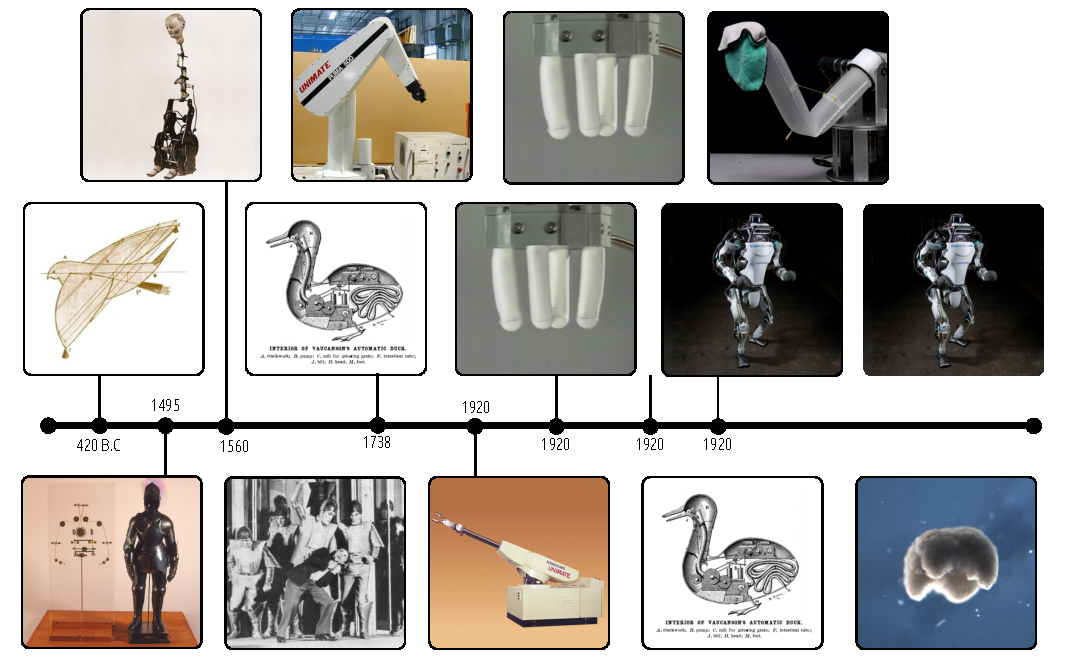
\includegraphics[width=1.11\textwidth]{./3_chapters/0_introduction/img/timeline.pdf}
\caption{A brief timeline of the state-of-the-art of robotics throughout human history. \textit{a)} One of the earliest examples of bio-mimicry -- the flying mechanical bird using steam-powered propulsion. \textit{b)} The Mechanical Knight by Leonardo Da Vinci. \textit{c)} Digesting duck patent of Jacques de Vaucanson. \textit{d)} The science-fiction play by Karel \v{C}apek on robots, who introduced the word \emph{robot} into the Oxford English Dictionary originally from his brother Josef \v{C}apek. \textit{f)} The first soft robot called Orm designed by V. Scheinman and L. Leifer. \textit{g)} The first redundant snake-like robot called Scripps tensor arm patented by V.C Anderson. }
\end{figure}
\clearpage
}

One of the earliest examples of bio-mimicry is a mechanical wooden dove developed by mathematician Archytas of Tarentum in 350 BC. According to historians, the system was driven by compressed air or an internal steam-driven engine to achieve forward propulsion, capable of traveling distances of \textapprox200 \si{\meter} (see note\footnote{It was unclear if the devices was attached to a rope, or autonomous flight was achieved.}). Archytas's invention could be considered as one of the earliest robotic systems -- a machine or device that operates automatically or by remote control -- whose main principles are somewhat analogous to nowadays \emph{drone} technology.  A millennium later, in the period of the High Renaissance, Leonardo da Vinci designed and constructed a mechanical knight around the 1490's. Such mechanical constructions were perhaps closer to conventional rigid robotics given our current robotics perspective. It is well-known that his work was built upon extensive anatomical research, which may have facilitated a deep understanding of the human body into the mechanical knight's robotic design.

\par In the 1920's, shortly after the second industrial revolution (1870 - 1914) and the first world war (1914), the first usage of the work \emph{robot} appeared -- originally meaning 'forced labor by serfs' (\ie, peasants) derived from the Czech word \emph{robota}. An common misconception is that robot implies slave, nonetheless, its origin is somewhat related. The word was popularized by Karel \v{C}apek in his play R.U.R. (Rossum’s Universal Robots) that involves an inventor named Rossum who discovers the secret of creating human-like machines. In his play, Rossom's robots assisted or fully alleviated mankind from any labor. Through human's ambition to assimilate man and machine, the robots ultimately gained the capacity for emotions. Shortly after, the robots, who were created to serve humans, have come to dominate mankind completely. The word \emph{robotics} was later solidified by Isaac Asimov, adapting the term from \v{C}apek. These works of science fiction are perhaps the fundamental groundwork of modern robotics which have led to the base practices of robotics and its corresponding academic field.

Only three decades later, in the 1950's, the first robotic arm called the 'Unimate' was employed in industry. The robot was used for manipulating metal die-casts and welding these to welding these to the main body of automobiles. Interestingly, the robot explored both electric as hydraulic-mechanical actuation, similar to nowadays popular Atlas robot (2013) by the company Boston Dynamics. Note that these robots were still controlled remotely, and rudimentary levels of closed-loop control were applied then. The 1950's also brought forth the McKibben actuators developed by Joseph Laws McKibben -- a well-known work in the field of soft robotics. These McKibben actuator consists of an inflatable inner bladder enveloped with a double-helical weave. When pressurized, the fluidic actuator converted radial expansion into uni-axial contraction since weave inhibited extensive \emph{ballooning} -- a term for undesired radial expansion. The McKibben actuators are perhaps seen as one of the first fundamental technologies that enabled soft robotics and to this day it remains a framework for many soft artificial muscle. Nevertheless, besides fluidics, there exist many other technologies employed in soft robotic motion that predate the invention of the McKibben actuator: such as thermal or chemical expansion/contraction, re-alignment of crystals, di-electric elastomers, magnetism, and naturally electro-mechanical actuation. For instance, the earliest system resambling Dielectric Elastomer Actuators (DEA) were developed W. C. R\"{o}ntgen in 1880. Although these mechanisms do not fall under the class soft robot, they are; however, categorized as soft actuators. We like to emphasize here the difference between soft actuators and soft robots in view of a terminology corresponding with the thesis:
%
\terminology{Soft actuators}{ are controllable flexible components of the constitutive soft robotic system that through external stimuli allow for motion or adaptability of compliance and/or texture.}
%
\noindent The terminology above attempts to address a common ambiguity in the field of soft robotics, that being interchangeably usage the term soft actuator and soft robot.

In 1965, the work of V. Scheinman and L. Leifer proposed a novel pneumatic robot arm named Orm -- the Norwegian word for snake. To the author's knowledge, this pneumatic robot is one of the first soft robots -- and suprisingly the system predates the first rigid redundant snake-like robots (1968). Similar to the anatomy of the snakes, the system featured 28 rubber pneumatic artificial muscle (\ie, bellows) distrubuted along the backbone (\ie, skeletal support) of the robot. The network of artificial muscles were sandwiched between steel plates to prevent disalignment. The soft robotic system could undergo three-dimensional movement by inflation or deflation of embedded pneumatic network, leading to a rich set of movements unseen in earlier robotics. The soft robot can achieve bending in any preferred direction by differential pressurization of each channel, and elongation through synchronized actuation. However, according to \cite{}, the positional accuracy of the system was poor, yet the concept of pneumatically-driven soft arms has continued. Two years later, In 1968, V.C. Anderson developed and patented one of the earliest hyper-redundant robotic manipulators.

\clearpage
\section{State-of-the-art in Soft Robotics}

\section{Problem statement}

\section{Research challenges and contribution}
\noindent \textbf{Design (Optimization)}.
\contribution{blaa}

\contribution{Validation of the proposed computational design algorithms Additive Manufacturing (AM) technologies.}

\noindent \textbf{Hyper-redundant Modeling}.
\contribution{blaa}

\noindent \textbf{Control and state estimation}.
\contribution{Development of energy-based control strategies applicable to continuum soft robotic manipulators as to allow for set-point stabilization, tracking, and grasping tasks.}

\noindent \textbf{Experimental applicability}.
\contribution{blaa}

\section{Outline of the thesis}

% \begin{figure}[t]
% \centering
% 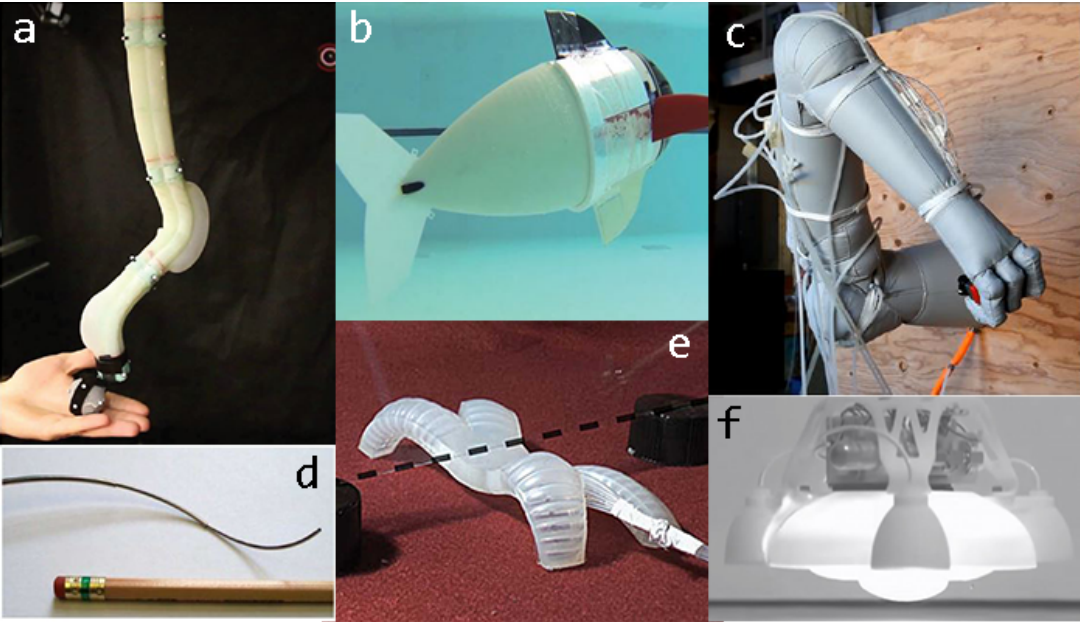
\includegraphics[width=0.98\textwidth]{./3_chapters/0_introduction/img/modern_softrobots.png}
% \caption{\textit{a)} Elepant-inspired trunk [14]. \textit{b)}, Fish-inspired aquatic robot [19]. \textit{c)}, Soft-infalatable human robot arm [13]. \textit{d)}, Concentric-tube hard continuum robot[21]. \textit{e)}, Soft quadruped robot [20]. \textit{f)}. Explosion- driven semi-soft 3D printed robot [22]. }
% \end{figure}

% Perhaps a subtle point in the terminology above, is its mention to biology.
% Although the area of soft robotics has grown exponentially since the early 2010's, the field of soft robotics dates back to the early 60's.

% \begin{figure}
% \centering
% \setlength\figurewidth{0.53\textwidth}
% \setlength\figureheight{0.25\textwidth}
% \input{./3_chapters/0_introduction/img/myfigure.tikz}
% \end{figure}

%\subsection{REF}

The first robotic manipulator arm used in the orbital environment was the Space Shuttle remote manipulator system. It was successfully demonstrated in the STS-2 mission in 1981 and is still operational today.

First soft robot: Victor Scheinman and Larry Leifer developed an air-powered robot arm called Orm, which is the Norwegian word for snake.

\begin{itemize}
  \item . F. Shulte, "The Characteristics of the Mckibben Artificial Muscle", The Application of External Power in Prosthetics and Orthetics, pp. 94-115, 1960.
  \item A. Chen, R. Yin, L. Cao, C. Yuan, H. K. Ding and W. J. Zhang, "Soft robotics: Definition and research issues," 2017 24th International Conference on Mechatronics and Machine Vision in Practice (M2VIP), 2017, pp. 366-370, doi: 10.1109/M2VIP.2017.8267170.
  \item  W. C. R\"{o}ntgen, “Ueber die durch Electricität bewirkten Form—und Volumenänderungen von dielectrischen Körpern,” Ann Phys Chem, no. 11, pp. 771-786, 1880.
\end{itemize}


%%%% Design
\cleardoublepage
\part{Design Optimization}\label{part: design}
%!TEX root = ../../thesis.tex
%%%% CHAPTER 1 *****************************************************************
\chapter[Design Optimization]{Optimal Design of Soft Robots -- a Gradient-based Approach}
\label{chap: chapter 2}

\blankfootnote{This chapter is based on:\\ .\disclaimer}

%%%% ABSTRACT ******************************************************************
%!TEX root = ../../thesis.tex
\chapterabstract{The motion complexity and use of exotic materials in soft robotics call for accurate and computationally efficient models intended for control. To reduce the gap between material and control-oriented research, we build upon the existing Piecewise-Constant Curvature framework by incorporating hyper-elastic and visco-elastic material behavior. In this work, the continuum dynamics of the soft robot are derived through the differential geometry of spatial curves, which are then related to Finite-Element data to capture the intrinsic geometric and material nonlinearities. To enable fast simulations, a reduced-order integration scheme is introduced to compute the dynamic Lagrangian matrices efficiently, which in turn allows for real-time (multi-link) models with sufficient numerical precision. By exploring the passivity and using the parametrization of the hyper-elastic model, we propose a passivity-based adaptive controller that enhances robustness towards material uncertainty and unmodeled dynamics -- slowly improving their estimates online. As a study case, a fully 3D-printed soft robot manipulator is developed, which shows good correspondence with the dynamic model under various conditions, e.g., natural oscillations, forced inputs, and under tip-loads. The solidity of the approach is demonstrated through extensive simulations, numerical benchmarks, and experimental validations.}


%%%% MAIN **********************************************************************
\section{Introduction} \label{sec: chap1 1_introduction}
%!TEX root = ../../thesis.tex
The field of soft robotics has attracted the interest of many researchers from different backgrounds. Soft robots use compliant and hyper-elastic materials, while the use of rigid materials is minimized. The introduction of soft materials into robotics greatly expanded the field of application for robotics. For example, due to their dexterity and environmental robustness, soft robots are often used in medical applications \cite{Polygerinos2015b, Yap2015, Asbeck2015}, adaptive grasping \cite{Galloway2016, Hughes2016}, and locomotion in uncertain environments \cite{Drotman2017}. Unlike its rigid counterpart, soft robots undergo large continuum-bodied motion that, to some extent, resembles morphologies found in nature. These morphologies arise by virtue of the low compliance in soft materials and, more importantly, the structural layout of the soft robot. As of today, many of the fundamental engineering principles in rigid robotics, like design, actuation, sensing, and control, are often not applicable to soft robotics systems. Since its inception, most of these engineering problems have remained challenging or unresolved.

Although the diversity in soft robotics is significant, ranging from adaptive grippers to soft manipulators, most topologies in soft robotics can be associated with nature or engineered geometries for minimal compliance (e.g., bellow shapes). Soft robots often mimic living creatures and their morphologies, e.g., the tentacle of an octopus \cite{Galloway2016, Wehner2016}, or the trunk of an elephant \cite{Drotman2017}. Hypothetically, the abundance of bio-mimicry in soft robotics might be associated with the design complexity of developing robots from soft materials. The large number of degrees-of-freedom and exotic mechanical nature of soft robots makes design significantly challenging, and consequently, the design process can be iterative and time-consuming \cite{Wehner2016}. Therefore, it becomes potentially advantageous to use computational tools that assist or develop appropriate soft robotic topologies given a set of user-defined requirements, like desired motion or force.

In the past, researchers have made efforts to finding morphologies through mathematics, in particular through evolutionary algorithms. The concept of automated creature designs was first introduced by Sims \cite{Sims1994}, who showed that, given a set of basic geometries, locomotive organisms could be generated from evolutionary algorithms. These virtual organisms resembled biological morphologies to some extent; however, the complexity of the material layout was limited. More recent work involving the synthesis of virtual soft robots includes Cheney et al. \cite{Cheney2013}, who successfully produced intricate locomotive morphologies using artificial neural networks and multi-material parameter spaces of active and passive soft voxels. Other work involving morphological synthesis includes \cite{Bern2019, Morzadec2019,Diepen2019}. Unfortunately, the synthesis of morphologies from previous approaches, though novel, remains only in ideal simulated environments. An accurate representation of the nonlinear material properties in soft robotics can be challenging, and in favor of computational efficiency, little detail is spent on the nonlinear nature governing soft materials. Besides, these evolutionary frameworks typically involve a network of `activation' cells or voxels that perform ideal volumetric deformation, biologically resembling muscle functionality while unfortunately lacking resemblance to conventional actuation in soft robotics, e.g., pneumatics, dielectrics, and smart metal alloys (SMA).

Reviewing previous methods, a more efficient approach for solving the optimal morphology might be founded in topology optimization. Topology optimization is the general formulation of a material distribution problem for mechanical solids, where density-based topologies arise throughout an iterative (non-convex) optimization procedure. The synthesis of compliant mechanisms through topology optimization is investigated thoroughly \cite{Sigmund2015, Gain2013, Luo2015}; however, its application to soft robotics is relatively unexplored \cite{Zhang2018,Zolfagharian2019}. Yet, to obtain meaningful topologies for soft robotics, two problems need to be addressed. Since soft robots undergo large deformations, it becomes necessary to describe the nonlinear geometrical deformations accurately. Inherent to significant deformation of soft materials is the importance of nonlinear material behavior, like hyperelasticity. Another concern is the design-dependency of the external forces, in our case, the pneumatic loads. This class of structural problems is more challenging than traditional problems since the load is continuously interacting with the adaptive interface during the iterative optimization process \cite{Wang2016, Vasista2013}. It should be mentioned that the use of compressed air or pressurized fluid is a popular actuation approach in soft robotics.

In this work, we present a novel framework for generating topologies of soft robotics. Contrary to biometry or convectional designs, finding the (optimal) material layout of the soft robot is accomplished through a gradient-based nonlinear topology optimization, where the distribution of soft materials is optimized given a user-defined objective. Our main contributions include the description of nonlinear geometrical deformation and pneumatic loading. We exploit the connectivity properties in polygonal meshes such that synchronized volumetric contraction or expansion of a group of polygonal elements can artificially mimic the geometrical loads in pneumatic actuation. The advantages of our framework in comparison to other literature are: ($i$) a better representation of pneumatic actuation in soft robotics; ($ii$) improved design convergence in contrast to evolution-based optimization methods. To our knowledge, our approach of pressure-driven nonlinear topology optimization is new for soft robotics, and its application could easily extend to other soft robotic systems. %The computational framework detailed in this work is made publicly available at \cite{Caasenbrood2019}.

The remainder of the paper is structured as follows. In section \ref{chap:fem}, we will discuss the continuum mechanics for hyper-elastic materials, followed by a description of the optimization scheme for soft robotics. In section \ref{chap:results}, we propose a numerical example for developing a soft robotic structure to illustrate the effectiveness of our approach.


%\section{Nonlinear Finite Elements} \label{sec: chap1 1_introduction}
%% \subsection{Strain theory in continuum mechanics}
% Here, we state the variational principle of continuum mechanics in a nonlinear geometrical setting. First, we introduce a description of the undeformed material domain described by $\mathcal{B}_0 \subset \R^3$. As external forces induce motion in $\mathcal{B}_0$, a representation of the deformed domain can be described by $\mathcal{B} \subset \R^3$. Suppose there exists an arbitrary material point inside the undeformed configuration represented by a position vector $\boldsymbol{X} \in \mathcal{B}_0$. Due to the motion of $\mathcal{B}_0$, a continuous path can be drawn between the position vectors $\boldsymbol{X}$ and $\boldsymbol{X}'$, that is, a particular material point in undeformed and deformed configuration, respectively. Therefore, let the deformation mapping for every material point in $\mathcal{B}_0$ be described by $\boldsymbol{\varphi}:\; \mathcal{B}_0 \to \mathcal{B}$ such that $\boldsymbol{X} \mapsto \boldsymbol{\varphi}(\boldsymbol{X}) = \boldsymbol{X}'$.
% Alternatively, we can write $\boldsymbol{X}' = \boldsymbol{\varphi}(\boldsymbol{X}) = \boldsymbol{X} + \boldsymbol{x}(\boldsymbol{X})$, where $\boldsymbol{x} \in \R^3$ is the displacement vector the material point Since the mapping $\boldsymbol{\varphi}$ is assumed to be sufficiently smooth, the second-order deformation gradient tensor is defined by
% \begin{equation}
% \boldsymbol{F} := \frac{\p \boldsymbol{\varphi} }{\p \boldsymbol{X}} \label{eq:F} = \boldsymbol{I} + \frac{\p \boldsymbol{x} }{\p \boldsymbol{X}}.
% \end{equation}
% The second-order deformation gradient tensor holds useful information about the deformation locally, i.e., it describes the deformation of an infinitesimal sub-volume of the material domain $\mathcal{B}_0$ around $\boldsymbol{X}$. From the deformation gradient, the Green-Lagrange strain tensor can be derived by $\boldsymbol{E} = \frac{1}{2}(\boldsymbol{C} - \boldsymbol{I})$, where $\boldsymbol{C} = \boldsymbol{F}^\tr \boldsymbol{F}$ is the right Cauchy-Green strain tensor. Expressed in terms of displacement gradient, the general expression for the second-order Green-Lagrange strain tensor becomes
% \begin{equation}
% \boldsymbol{E} = \frac{1}{2}\left( \frac{\p \boldsymbol{x}}{\p \boldsymbol{X}} + \frac{\p\boldsymbol{x}^\tr}{\p \boldsymbol{X}} + \frac{\p\boldsymbol{x}^\tr}{\p \boldsymbol{X}}\frac{\p\boldsymbol{x}}{\p \boldsymbol{X}} \right). \label{eq:E_tens}
% \end{equation}
% Since the numerical implementation generally involves matrix-vector notation instead of tensor notation; we briefly introduce the following notation. A Cartesian tensor can be formally represented by an component array in terms of a basis $\boldsymbol{e}_i$. For example, a second-order tensor can be denoted by $\boldsymbol{T} = \sum_{ij}\boldsymbol{T}_{ij}\, \boldsymbol{e}_i \kron \boldsymbol{e}_j$ with $\kron$ the dyadic product and bases $\boldsymbol{e}_1,\boldsymbol{e}_2,\boldsymbol{e}_3 \in \R^3$. As such, the column vector representation of a second-order tensor $\boldsymbol{T}$ can be denoted by $\{ \boldsymbol{T}\} := \text{vec}(\boldsymbol{T}_{ij})$. Hence, the variational form of Lagrangian strain can be written in vector notation as
% \begin{equation}
% \{d \boldsymbol{E} \}= \boldsymbol{B}(\boldsymbol{x}) \, \{d \boldsymbol{x}\},
% \end{equation}
% where $\boldsymbol{B}(\boldsymbol{x})$ is a nonlinear strain-displacement matrix that relates displacements to Lagrangian strain \cite{Kim2018}. In this work, we primarily focus on two-dimensional mechanical problems. We would like to stress that the variational principle for three-dimensional continuum solids discussed earlier are similar to those in two-dimensional situations \cite{Kim2018,Gain2013}.
%
% \subsection{Isotropic hyperelasticity}
% In soft robotics, the use of elastomer materials is widespread due to their relatively low Young's moduli, large reversible strains, and mechanical robustness. These elastic materials are distinguished in material mechanics as hyperelastic materials. The presence of large deformations and rubber-like materials inherently leads to a state-dependent mechanical compliance. In contrast to Hookean materials, whose elasticity is linear, the constitutive behavior of hyperelastic materials is described by a (nonlinear) strain energy function ${\Psi}: \R^{3\times3} \mapsto \Rp$, i.e., a mapping from the Lagrangian strain tensor to potential energy. Popular constitutive models for hyperelastic behavior include Neo-Hookean, Mooney, Ogden, or Yeoh. In contrast to linear elasticity strain energy, the strain energy for hyperelastic constitutive models are commonly expressed in terms of the strain invariants (${J}_1$, ${J}_2$, ${J}_3$).
%
% In this work, the Yeoh constitutive model for hyperelasticity is used to describe the mechanics of soft materials. The Yeoh model is a popular constitutive model due to its unique dependency on the first invariant $J_1 = \text{tr}(\boldsymbol{C})$. The strain energy function of the Yeoh model \cite{Kim2018} is given by
% \begin{equation}
% {\Psi} = \sum_{i = 1}^{3} c_i (J_1 - 3)^i,
% \end{equation}
% where $c_1 > 0$ and $c_2$, $c_3$ are material constants (J/m$^3$). The second Piola-Kirchoff stress of a constitutive material can be calculated by differentiating the strain energy function with respect to the Lagrangian strain tensor \cite{Renaud2011,Kim2018}
% \begin{equation}
% \boldsymbol{S} = \frac{\p {\Psi}}{\p \boldsymbol{E}} = 2\frac{\p {\Psi}}{\p \boldsymbol{C}},
% \label{eq:piola}
% \end{equation}
% which is a symmetric second-order tensor that is the energy conjugate to the Lagrangian strain. Suppose that the external forces acting on the boundary of the material domain $\mathcal{B}_0$ can be represented by the vector $\boldsymbol{f}$. Then, in case of a (quasi)-static equilibrium, the residual between the internal force of the continuum solids and the external forces can be written as
% \begin{equation}
% \boldsymbol{R(\boldsymbol{x})} = \int_{\mathcal{B}_0} \boldsymbol{B}(\boldsymbol{x})^\tr \{\boldsymbol{S}\}  \; dV -\boldsymbol{f} = 0, \label{eq:residual}
% \end{equation}
% where the first right-hand term represents a volume integral over the undeformed domain $\mathcal{B}_0$. Given the context of finite elements, this represents a set of nonlinear equalities with unknown nodal displacements $\boldsymbol{x}$. The solutions to these (highly) nonlinear equations can be found through numerical methods, like the Newton-Raphson method.



\cleardoublepage
\part{Modeling of Soft Robots}\label{part: model}
%!TEX root = ../../thesis.tex
%%%% CHAPTER 1 *****************************************************************
\chapter[Dynamic modeling of Soft Robots -- PCC case]{Dynamic modeling -- The  Constant Strain Approach}
\label{chap: chapter 1}

\blankfootnote{This chapter is based on:\\ .\disclaimer}

%%%% ABSTRACT ******************************************************************
%!TEX root = ../../thesis.tex
\chapterabstract{
%The motion complexity and use of exotic materials in soft robotics call for accurate and computationally efficient models intended for control. To reduce the gap between material and control-oriented research, we build upon the existing Piecewise-Constant Curvature framework by incorporating hyper-elastic and visco-elastic material behavior.
In this chapter, the continuum dynamics of the soft robot are derived through the differential geometry of spatial curves, which are then related to Finite-Element data to capture the intrinsic geometric and material nonlinearities. To accelerate numerical simulation, a reduced-order integration scheme is introduced to compute the dynamic Lagrangian matrices efficiently. This, in turn, allows for real-time (multi-link) models with sufficient numerical precision. By exploring the passivity and using the parametrization of the hyper-elastic model, we propose a passivity-based adaptive controller that enhances robustness towards material uncertainty and unmodeled dynamics -- slowly improving their estimates online. As a study case, a fully 3D-printed soft robot manipulator is developed, which shows good correspondence with the dynamic model under various conditions, \eg, natural oscillations, forced inputs, and subjected to external disturbances like tip-loads. The solidity of the approach is demonstrated through extensive simulations, numerical benchmarks, and experimental validations.}


%%%% MAIN **********************************************************************
\section{Introduction} \label{sec: chap1 1_introduction}
%!TEX root = ../../thesis.tex
Traditional robots are made from rigid and dense materials that ensure accurate and repeatable motions. While rigid robotics excel at fast and precise motion, their structural rigidity lacks the compliance and mechanical robustness needed for safe and passive interaction in an unknown environment. Soft robotics, on the other hand, aim to improve the motion complexity and environmental robustness that is generally lacking its rigid counterpart. To further promote these topics in robotics, researchers aim to mimic living creatures by developing bio-inspired robots with similar morphologies and mechanical properties \cite{Falkenhahn2015,Suzumori1991,Godage2015,Godage2016,Marchese2014,Kriegman2019}.
The hyper-flexible and continuum-bodied structure in soft robots provides them with a rich family of motion primitives. Besides bio-mimicry, soft robotics has proven to be a prominent alternative for rigid robotics with a variety of applications, \eg, manipulation and adaptive grasping \cite{Galloway2016}, untethered locomotion and exploration through uncertain environments \cite{Marchese2014,Choi2011,Pilz2020}, rehabilitation \cite{Polygerinos2015}, and even minimal-invasive surgery \cite{Li2017a,Cianchetti2014}. Although the popularity of the field has increased exponentially in recent years, one of the first soft robots dates back already to the early 1990s, \eg, the work of Suzumori et al. (1991, \cite{Suzumori1991}). Yet, despite years of soft robotics research, their intrinsic hyper-flexible nature still possesses numerous challenges on modeling and control.

One major challenge in modeling is that the soft robot's elastic body undergoes large, continuous deformation. Since its inception, numerous works have addressed the kinematics for soft continuum robots \cite{Jones2006,Mochiyama1999,Mochiyama2003}; yet, its original framework stems from hyper-redundant robotics nearly a decade earlier \cite{Chirikjian1994}. Similar to soft robots, hyper-redundant robots exploit their high joint redundancy to achieve a broader range of tasks (\eg, shape control and collision avoidance) besides end-effector manipulation. To some extent, soft robots can be seen as the successor to hyper-redundant robots in which rigid mechanical joints or links are substituted with hyper-flexible soft elements. As a result, their dynamics involve a continuously deformable inertial body rather than the classical notion of rigid bodies. As such, conventional modeling approaches cannot be applied directly to these continuously deformable robots, stressing the importance of novel modeling strategies. In this respect, the dynamics of a continuously deformable soft robot are, in theory, of an infinite-dimensional nature. This paradigm shift has further emphasized the challenges in control-oriented modeling of soft robots, as their physical description are often more suited for a Partial-Differential Equations (PDEs) rather than Ordinary Differential Equations (ODEs).

Recently, some significant steps have been made toward formulating reduced-order ODE models for elastic continuum soft robots, paving a path toward model-based controllers. Perhaps one of the most popular techniques of spatial reduction is the so-called \textit{"Piece-wise Constant Curvature"} model or PCC for short. The PCC model assumes that a soft robot's reachability can be described using a number of spatially-constant curves, which are parameterized using a minimal set of generalized coordinates. Although PCC models can be seen as a significant oversimplification of true continuum mechanics at hand, these models have proven to be remarkably viable for various control applications. Besides its use in inverse kinematic control \cite{Marchese2014,Marchese2016,Jones2006}, PCC models have also shown to be suitable for feedforward controllers as demonstrated by Falkenhahn et al. (2015, \cite{Falkenhahn2015}); and more recently, closed-loop feedback controllers by Della Santina et al. (2019-2020, \cite{DellaSantina2020,Katzschmann2019}). Although the aforementioned works utilize the lumped-mass description, others have employed PCC models with uniform mass distribution \cite{Renda2018,Godage2015,Godage2016,Tatlicioglu2007,Tatlicioglu2007a} and current models even extend beyond the constant curvature \cite{Mochiyama2003,Chirikjian1994,DellaSantina2020}. However, in the face of significant external loading or (distributed) contact with the environment, the PCC assumption is relatively conservative and leads to undesired kinematic constraints on the continuum deformation. Besides, these models often need additional identification to model compliance as they do not originate from a continuum mechanical framework.

On the other hand, Finite-Element Method (FEM) models do originate from continuum mechanics and, due to their PDE description, provide a more accurate representation of deformations; and are particularly suited to deal with geometric and material nonlinearities. Duriez et al. (2013, \cite{Duriez2013}) and related works \cite{Coevoet2017,Largilliere2015,Goury2018} showed that reduced-order FEM models could play an important role in closed-loop control -- allowing accurate volumetric deformation and hyper-elastic behavior. Although such real-time simulations for FEM-based models are possible, a significant state-reduction is required to ensure sufficient computational speed. In the process, FEM-based models often lose desirable control properties, \eg, passivity preservation, which might play an important role in control. An alternative modeling strategy is the recently emerging geometrically-exact Cosserat-beam model. Similar to the PCC models, the Cosserat models have the merit benefit that they can be structured into a standard Lagrangian form -- the basis for robotics control theory. Rooted in a geometric method for describing the continuum mechanics using Lie theory proposed by Simo et al. (1986, \cite{Simo1986}), Boyer et al. (2021, \cite{Boyer2010, Boyer2021}) proposed a geometrically-exact modeling framework for Cosserat beams using nonlinear parametrization of the strain field. Other examples include the work of Renda et al. (2018, \cite{Renda2018,Renda2020}), providing various options for Piecewise-Constant Strain (PCS) and Variable Strain modeling approaches. Although recent variants of the Cosserat models offer good computational performance \cite{Till2019,Grazioso2019}, its use in model-based control is slowly upcoming.

In this respect, the topic of reduced-order modeling of soft robots is an active area of research. Yet, a challenge that is frequently overlooked in control-orientated research is the anisotropic material behavior, mechanical saturation, and more importantly, the nonlinear and possibly time-varying nature of the highly hyper-elastic soft materials \cite{Falkenhahn2015, Mochiyama2003, Till2019, Tatlicioglu2007}. This is further amplified by the fact that soft robots are known for their diversity in elastic materials and corresponding morphologies. Mustaza et al. (2019, \cite{Mustaza2019}) proposed a modified nonlinear Kelvin-Voigt material model to embody the complex material behavior of silicone-composite manipulators (so-called STIFF-FLOP actuators). A similar silicone composite actuator was experimentally validated by Sadati et al. (2020, \cite{Sadati2020}) who proposed a novel modeling approach with an appendage-dependent Hookean model and viscous power-law to describe nonlinear and time-dependent material effects, respectively. Both nonlinear material models show good correspondence with physical soft robots under various dynamic conditions, yet they lack general transferability to the soft robots with different geometries -- intrinsically captured by FEM-driven models. As of today, there are few control-oriented models that both offer geometry and material versatilely similar to FEM models and the control convenience similar to spatial curve models.

Ultimately, the strong nonlinearities paired with its continuous nature encourage the use of model-based controllers. Nevertheless, regarding the aforementioned model-based control approaches \cite{DellaSantina2020,Katzschmann2019,Falkenhahn2015}, the stability and performance of the closed-loop system could be undermined by uncertainties in physical parameters or unmodelled dynamics. Particularly for state-feedback linearization (e.g., inverse dynamic), as the inversion of inaccurately estimated systems could lead to poor performance and even instability. Adaptive control \cite{Slotine1988,Morgan1977} or energy-based controllers \cite{Ortega1998} might offer the needed robustness towards material uncertainties and unmodelled dynamics. Unfortunately, up till now, the applicability of adaptive and energy-based control techniques on soft robotics is scarcely explored. Franco et al. (2020, \cite{Franco2020}) used an adaptive energy-based controller that compensates for external disturbances on the end-effector, yet this controller can be extended to include various slowly-varying material uncertainties, \eg, hyper-elasticity and viscosity.

The contributions of the work are two-fold. First, to derive a finite-dimensional dynamic model of a continuum soft robot, where we briefly recapitulate existing modeling techniques for soft robot manipulators. To address the issue of infinite-dimensionality, we explore the PCC condition that allows for a low-dimensional description of the continuum dynamics. Although such modeling approaches have been thoroughly developed, we will address two issues that will aid the development of model-based controllers. We aim to bridge the gap between the PCC model and the underlying continuum mechanics by matching the quasi-static behavior to a Finite-Element-driven model (FEM), and we propose a reduced-order integration scheme using Matrix-Differential Equations (MDEs) to compute the spatio-temporal dynamics in real-time. Preliminary results of this work were shown in Caasenbrood et al. (2020, \cite{Caasenbrood2020}) and in Caasenbrood et al. (2022, \cite{}).
%

Second, in regards to the FEM-based hyper-elastic modeling and the possible presence of unmodelled dynamics (e.g., material uncertainties or external loads on the end-effector), a passivity-based adaptive controller is proposed that enhances robustness towards material uncertainties and unmodelled dynamics in closed-loop, slowly improving their estimates online. All source code is made publicly available at Caasenbrood et al. (2020, \cite{SorotokiCode}).%\highlight{(see the open software repository)}

\section{System development}
By using additive manufacturing, we developed a soft and flexible robot manipulator that is suitable for pick-and-place applications. The 3-DOF soft robot can be seen in Figure \ref{fig:C2:soft_robot}. The soft robot manipulator in this work is loosely inspired by the elephant whose trunk-appendage consists mainly of parallel muscles without skeletal support. The anatomy of the elephant's trunk provides an excellent study case, as they naturally exhibit continuum-body bending and moderate elongation \cite{Falkenhahn2015,Jones2006,Tatlicioglu2007}. Similar to the earlier soft robotic designs
\cite{Suzumori1991,Falkenhahn2015}, the developed soft robot can undergo three-dimensional movement by inflation or deflation of embedded pneumatic bellow network. The pneumatic network has three unique inputs, which labeled $\uB = (u_1,\,u_2,\,u_3)^\top$. By varying the input $\uB$, the soft robot can achieve bending in any preferred direction by differential pressurization of each channel ($<$0.1 \si{\mega \pascal}), \eg, $u_1 > u_2 = u_3 > 0$. Whereas, simultaneous pressurization accomplishes moderate elongation, \ie, $u_1 = u_2 = u_3$. As a demonstration, we provided the following pressure inputs to the system:
%
\begin{align}
  u_i(t) = \begin{cases}
          \;\;\erf(t)\cdot \left[P_0 - P_a\sin\left(\pi t + \delta\right)\right] \quad\;\; \textrm{for}\;\; i = 1,2 \\[0.35em]
          \;\;\erf(t)\cdot \left[P_0 - P_a\sin\left(\pi t \right)\right] \quad\quad\quad\;\; \textrm{otherwise}\;\ \\
           \end{cases}
\end{align}
%
where $P_0 = 5$ \si{\kilo \pascal}, $P_a = 15$ \si{\kilo \pascal}, $\delta = \frac{\pi}{2}$, and $\textrm{erf}(t) := \frac{2}{\pi}\int_0^\tau \exp(-\tau^2) \; d\tau$   the error function to ensure a smooth transient. The demonstration is shown in Figure \ref{fig:C2:soft_robot}.

%
\begin{figure}[!h]
 \vspace{-3mm}
  \centering
  \ifx\printFigures\undefined
  \else
  % This file was created by matlab2tikz.
%
\begin{tikzpicture}

\begin{axis}[%
width=0.712\textwidth,
height=0.249\textwidth,
at={(0.11\textwidth,0\textwidth)},
scale only axis,
xmin=0,
xmax=1,
ymin=0,
ymax=1,
axis line style={draw=none},
ticks=none,
axis x line*=bottom,
axis y line*=left,
colorbar style={width=6,xshift=-7.5pt}
]
\end{axis}

\begin{axis}[%
width=0.204\textwidth,
height=0.204\textwidth,
at={(0\textwidth,0.031\textwidth)},
scale only axis,
axis on top,
xmin=0.5,
xmax=796.5,
tick align=outside,
y dir=reverse,
ymin=0.5,
ymax=796.5,
axis line style={draw=none},
ticks=none,
colorbar style={width=6,xshift=-7.5pt}
]
\addplot [forget plot] graphics [xmin=0.5, xmax=796.5, ymin=0.5, ymax=796.5] {fig_C2_srm_example-1.png};
\end{axis}

\begin{axis}[%
width=0.204\textwidth,
height=0.204\textwidth,
at={(0.232\textwidth,0.031\textwidth)},
scale only axis,
axis on top,
xmin=0.5,
xmax=796.5,
tick align=outside,
y dir=reverse,
ymin=0.5,
ymax=796.5,
axis line style={draw=none},
ticks=none,
colorbar style={width=6,xshift=-7.5pt}
]
\addplot [forget plot] graphics [xmin=0.5, xmax=796.5, ymin=0.5, ymax=796.5] {fig_C2_srm_example-2.png};
\end{axis}

\begin{axis}[%
width=0.204\textwidth,
height=0.204\textwidth,
at={(0.464\textwidth,0.031\textwidth)},
scale only axis,
axis on top,
xmin=0.5,
xmax=796.5,
tick align=outside,
y dir=reverse,
ymin=0.5,
ymax=796.5,
axis line style={draw=none},
ticks=none,
colorbar style={width=6,xshift=-7.5pt}
]
\addplot [forget plot] graphics [xmin=0.5, xmax=796.5, ymin=0.5, ymax=796.5] {fig_C2_srm_example-3.png};
\end{axis}

\begin{axis}[%
width=0.204\textwidth,
height=0.205\textwidth,
at={(0.696\textwidth,0.03\textwidth)},
scale only axis,
axis on top,
xmin=0,
xmax=796.5,
xtick={0,500},
xticklabels={\empty},
tick align=outside,
y dir=reverse,
ymin=0,
ymax=800,
ytick={0,200,400,600,800},
yticklabels={\empty},
axis line style={draw=none},
ticks=none,
axis x line*=bottom,
axis y line*=left,
colorbar style={width=6,xshift=-7.5pt}
]
\addplot [forget plot] graphics [xmin=0.5, xmax=796.5, ymin=0.5, ymax=796.5] {fig_C2_srm_example-4.png};
\end{axis}
\end{tikzpicture}%
   \vspace{2mm}
  % This file was created by matlab2tikz.
%
\begin{tikzpicture}

\begin{axis}[%
width=0.712\textwidth,
height=0.249\textwidth,
at={(0.11\textwidth,0\textwidth)},
scale only axis,
xmin=0,
xmax=1,
ymin=0,
ymax=1,
axis line style={draw=none},
ticks=none,
axis x line*=bottom,
axis y line*=left,
colorbar style={width=6,xshift=-7.5pt}
]
\end{axis}

\begin{axis}[%
width=0.204\textwidth,
height=0.204\textwidth,
at={(0.232\textwidth,0.03\textwidth)},
scale only axis,
axis on top,
xmin=0.5,
xmax=796.5,
tick align=outside,
y dir=reverse,
ymin=0.5,
ymax=796.5,
axis line style={draw=none},
ticks=none,
colorbar style={width=6,xshift=-7.5pt}
]
\addplot [forget plot] graphics [xmin=0.5, xmax=796.5, ymin=0.5, ymax=796.5] {fig_C2_srm_example_2-1.png};
\end{axis}

\begin{axis}[%
width=0.204\textwidth,
height=0.204\textwidth,
at={(0.464\textwidth,0.03\textwidth)},
scale only axis,
axis on top,
xmin=0.5,
xmax=796.5,
tick align=outside,
y dir=reverse,
ymin=0.5,
ymax=796.5,
axis line style={draw=none},
ticks=none,
colorbar style={width=6,xshift=-7.5pt}
]
\addplot [forget plot] graphics [xmin=0.5, xmax=796.5, ymin=0.5, ymax=796.5] {fig_C2_srm_example_2-2.png};
\end{axis}

\begin{axis}[%
width=0.204\textwidth,
height=0.204\textwidth,
at={(0\textwidth,0.03\textwidth)},
scale only axis,
axis on top,
xmin=0.5,
xmax=796.5,
tick align=outside,
y dir=reverse,
ymin=0.5,
ymax=796.5,
axis line style={draw=none},
ticks=none,
colorbar style={width=6,xshift=-7.5pt}
]
\addplot [forget plot] graphics [xmin=0.5, xmax=796.5, ymin=0.5, ymax=796.5] {fig_C2_srm_example_2-3.png};
\end{axis}

\begin{axis}[%
width=0.204\textwidth,
height=0.205\textwidth,
at={(0.696\textwidth,0.03\textwidth)},
scale only axis,
axis on top,
xmin=0,
xmax=796.5,
xtick={0,500},
xticklabels={\empty},
tick align=outside,
y dir=reverse,
ymin=0,
ymax=800,
ytick={0,200,400,600,800},
yticklabels={\empty},
axis line style={draw=none},
ticks=none,
axis x line*=bottom,
axis y line*=left,
colorbar style={width=6,xshift=-7.5pt}
]
\addplot [forget plot] graphics [xmin=0.5, xmax=796.5, ymin=0.5, ymax=796.5] {fig_C2_srm_example_2-4.png};
\end{axis}
\end{tikzpicture}%
  \vspace{-3mm}
  % This file was created by matlab2tikz.
%
\definecolor{mycolor1}{rgb}{0.00000,0.34510,0.65882}%
\definecolor{mycolor2}{rgb}{0.79216,0.11765,0.17255}%
\definecolor{mycolor3}{rgb}{0.20392,0.65490,0.24706}%
%
\begin{tikzpicture}

\begin{axis}[%
width=0.8\textwidth,
height=0.179\textwidth,
at={(0\textwidth,0\textwidth)},
scale only axis,
xmin=0,
xmax=10,
xlabel style={font=\color{white!15!black}},
xlabel={time (s)},
ymin=-20,
ymax=40,
ylabel style={font=\color{white!15!black}},
ylabel={$\textit{\textbf{u}}\,(t)$ (kPa)},
axis background/.style={fill=white},
xmajorgrids,
ymajorgrids,
ylabel style={yshift=-7.5pt}
]
\addplot [color=mycolor1, line width=1.5pt, forget plot]
  table[row sep=crcr]{%
0	-0\\
0.0800800800800801	-0.326421096773199\\
0.13013013013013	-0.446396146969825\\
0.16016016016016	-0.475915059812738\\
0.19019019019019	-0.468617984138909\\
0.22022022022022	-0.421114993853074\\
0.26026026026026	-0.290581235653967\\
0.31031031031031	-0.0133501719664331\\
0.37037037037037	0.490936189786673\\
0.44044044044044	1.30870274857828\\
0.53053053053053	2.67542755986546\\
0.67067067067067	5.2362166600556\\
0.830830830830831	8.06311411354436\\
0.910910910910911	9.10605922484043\\
0.970970970970971	9.61807923316933\\
1.01101101101101	9.80511023254271\\
1.04104104104104	9.85652001840668\\
1.06106106106106	9.8464167830638\\
1.08108108108108	9.79979543095045\\
1.11111111111111	9.65996707165884\\
1.15115115115115	9.34097577727256\\
1.2012012012012	8.72856335397239\\
1.26126126126126	7.68842452977073\\
1.34134134134134	5.82705175209153\\
1.44144144144144	2.89025349032573\\
1.78178178178178	-7.66126479630216\\
1.85185185185185	-8.93823786685945\\
1.9019019019019	-9.48537113895998\\
1.93193193193193	-9.65018897998966\\
1.95195195195195	-9.68800064376008\\
1.97197197197197	-9.66633786975596\\
1.99199199199199	-9.58391156057349\\
2.01201201201201	-9.38332861181659\\
2.06206206206206	-8.53932967412129\\
2.12212212212212	-7.08800557275741\\
2.2022022022022	-4.4965915337584\\
2.3023023023023	-0.439410784019138\\
2.69269269269269	16.3221257528725\\
2.77277277277277	18.415013753162\\
2.83283283283283	19.4356806473722\\
2.87287287287287	19.8329494125197\\
2.9029029029029	19.9772856135889\\
2.92292292292292	19.9995372186649\\
2.94294294294294	19.9624739715968\\
2.97297297297297	19.7960483764044\\
3.01301301301301	19.3698711750903\\
3.06306306306306	18.5189587240366\\
3.12312312312312	17.0600160253529\\
3.2032032032032	14.4600311678918\\
3.31331331331331	9.95268952377332\\
3.67367367367367	-5.71438002463892\\
3.75375375375375	-7.99033138710941\\
3.81381381381381	-9.16654342890359\\
3.86386386386386	-9.76383453862231\\
3.9039039039039	-9.97980651362566\\
3.92392392392392	-9.99909251603334\\
3.94394394394394	-9.95906542484922\\
3.97397397397397	-9.7882229857449\\
4.01401401401402	-9.35627162946138\\
4.06406406406407	-8.49845408003308\\
4.12412412412413	-7.03190721204662\\
4.20420420420421	-4.42337724832305\\
4.31431431431432	0.0918605166913373\\
4.67467467467468	15.7473395539602\\
4.75475475475476	18.0138529161429\\
4.81481481481482	19.1819782322969\\
4.86486486486487	19.7720990448672\\
4.8948948948949	19.9517886445088\\
4.91491491491492	19.9977546859628\\
4.93493493493494	19.9844129242011\\
4.95495495495496	19.9118161184931\\
4.98498498498499	19.692509501943\\
5.02502502502503	19.1973369064934\\
5.07507507507508	18.264138133125\\
5.14514514514515	16.4145743346791\\
5.22522522522523	13.6326840302821\\
5.34534534534535	8.50521702792188\\
5.63563563563564	-4.38647516760632\\
5.72572572572573	-7.28045577289802\\
5.7957957957958	-8.86491478632072\\
5.84584584584585	-9.59019275917794\\
5.88588588588589	-9.91179460555106\\
5.91591591591592	-9.99849667044506\\
5.93593593593594	-9.98218895327441\\
5.95595595595596	-9.90663498672929\\
5.98598598598599	-9.68293467832493\\
6.02602602602603	-9.18204294489704\\
6.07607607607608	-8.24204535487507\\
6.14614614614615	-6.38391405917885\\
6.22622622622623	-3.59406523774787\\
6.34634634634635	1.54066527788336\\
6.63663663663664	14.423222670133\\
6.72672672672673	17.3074818400554\\
6.7967967967968	18.8828466654283\\
6.84684684684685	19.6010714539438\\
6.88688688688689	19.9168288901412\\
6.91691691691692	19.9990903293176\\
6.93693693693694	19.979816818011\\
6.95695695695696	19.9013064378096\\
6.98698698698699	19.6732146498049\\
7.02702702702703	19.1666087318999\\
7.07707707707708	18.2198216212038\\
7.14714714714715	16.3531412039961\\
7.22722722722723	13.5553614553648\\
7.34734734734735	8.4134182056872\\
7.63763763763764	-4.45987698297003\\
7.72772772772773	-7.33438619403134\\
7.7977977977978	-8.90064125199644\\
7.84784784784785	-9.61180575338317\\
7.88788788788789	-9.92171565676419\\
7.91791791791792	-9.99953565670966\\
7.93793793793794	-9.97729654186992\\
7.95795795795796	-9.89583052442988\\
7.98798798798799	-9.66334951250793\\
8.02802802802803	-9.15103442013677\\
8.07807807807808	-8.19746715188983\\
8.14814814814815	-6.32225607345482\\
8.23823823823824	-3.12412058064418\\
8.35835835835836	2.09379127496054\\
8.62862862862863	14.1266639802227\\
8.71871871871872	17.0878879354425\\
8.78878878878879	18.7355625082257\\
8.84884884884885	19.6223955513405\\
8.88888888888889	19.926454857093\\
8.91891891891892	19.9998326482171\\
8.93893893893894	19.974628149775\\
8.95895895895896	19.8902073007435\\
8.98898898898899	19.6533393639939\\
9.02902902902903	19.1353201636276\\
9.07907907907908	18.1749821680047\\
9.14914914914915	16.2912589729894\\
9.23923923923924	13.0844270116058\\
9.35935935935936	7.85991719202451\\
9.62962962962963	-4.16405358395558\\
9.71971971971972	-7.1157584442214\\
9.78978978978979	-8.75445039392143\\
9.84984984984985	-9.63284074308951\\
9.88988988988989	-9.93104644425996\\
9.91991991991992	-9.99998130090296\\
9.92992992992993	-9.99330959530174\\
9.94994994994995	-9.93550877769289\\
9.97997997997998	-9.7382022827042\\
10	-9.53368632565967\\
};
\addplot [color=mycolor2, line width=1.5pt, forget plot]
  table[row sep=crcr]{%
0	-0\\
0.11011011011011	-0.501631548802106\\
0.17017017017017	-0.672771725604441\\
0.21021021021021	-0.719575951069583\\
0.24024024024024	-0.711925105415364\\
0.27027027027027	-0.663529844709625\\
0.31031031031031	-0.530499096325073\\
0.36036036036036	-0.247084664731663\\
0.42042042042042	0.270928243995186\\
0.49049049049049	1.1163420287873\\
0.58058058058058	2.54202613740464\\
0.71071071071071	5.05316960834889\\
0.890890890890891	8.52020306455763\\
0.970970970970971	9.67944745678268\\
1.03103103103103	10.2735946634854\\
1.07107107107107	10.5113084593509\\
1.1011011011011	10.5979484020371\\
1.12112112112112	10.6097926348153\\
1.14114114114114	10.5837544842323\\
1.17117117117117	10.4719971670263\\
1.21121121121121	10.184624855263\\
1.26126126126126	9.60122488058117\\
1.32132132132132	8.57852016935115\\
1.39139139139139	6.97040405862983\\
1.48148148148148	4.34975735826455\\
1.63163163163163	-0.838417883808095\\
1.79179179179179	-6.18516552979148\\
1.88188188188188	-8.44875503362838\\
1.94194194194194	-9.46811471757773\\
1.99199199199199	-9.95523231675877\\
2.002002002002	-9.99970331978025\\
2.02202202202202	-9.96411589164284\\
2.05205205205205	-9.79989003331738\\
2.09209209209209	-9.37658932472964\\
2.14214214214214	-8.52911802342114\\
2.2022022022022	-7.07396678042702\\
2.28228228228228	-4.4782460740071\\
2.38238238238238	-0.417331272446525\\
2.77277277277277	16.3376476120192\\
2.85285285285285	18.425593622457\\
2.91291291291291	19.4420981038878\\
2.95295295295295	19.8364558610294\\
2.98298298298298	19.9785698881821\\
3.003003003003	19.9993324722562\\
3.02302302302302	19.9607810138446\\
3.05305305305305	19.7921374866907\\
3.09309309309309	19.3630605175579\\
3.14314314314314	18.5086799195633\\
3.2032032032032	17.0459173142334\\
3.28328328328328	14.4416386890202\\
3.39339339339339	9.93032677916854\\
3.75375375375375	-5.73094246460772\\
3.83383383383383	-8.00215775878589\\
3.89389389389389	-9.17431085668792\\
3.94394394394394	-9.76800245162413\\
3.97397397397397	-9.94988880393029\\
3.99399399399399	-9.9973299484371\\
4.01401401401402	-9.98546496932957\\
4.03403403403404	-9.91434078602069\\
4.06406406406407	-9.69722257406094\\
4.10410410410411	-9.20489933310494\\
4.15415415415416	-8.27508909582531\\
4.22422422422423	-6.42979782943817\\
4.30430430430431	-3.65188028723395\\
4.42442442442443	1.47195134180766\\
4.71471471471472	14.3681441665571\\
4.80480480480481	17.2669543507487\\
4.87487487487488	18.8559354690983\\
4.92492492492493	19.5847225103823\\
4.96496496496497	19.9092330715828\\
4.994994994995	19.9981457807168\\
5.01501501501502	19.983314776841\\
5.03503503503504	19.9092330715828\\
5.06506506506507	19.6877200825019\\
5.10510510510511	19.1896752583361\\
5.15515515515516	18.2530616010562\\
5.22522522522523	16.3991937198305\\
5.30530530530531	13.6133039531094\\
5.42542542542543	8.48218355487591\\
5.71571571571572	-4.40493793222117\\
5.80580580580581	-7.29404091858868\\
5.87587587587588	-8.87393563930486\\
5.92592592592593	-9.59567305869735\\
5.96596596596597	-9.91434078602069\\
5.995995995996	-9.99881329085688\\
6.01601601601602	-9.98101640888201\\
6.03603603603604	-9.90397791429554\\
6.06606606606607	-9.67807233871631\\
6.10610610610611	-9.17431085668794\\
6.15615615615616	-8.23090304192219\\
6.22622622622623	-6.36847687943411\\
6.30630630630631	-3.57464243887714\\
6.42642642642643	1.56371598502504\\
6.71671671671672	14.4416386890202\\
6.80680680680681	17.3210059061694\\
6.87687687687688	18.8917986050964\\
6.92692692692693	19.6064792650725\\
6.96696696696697	19.9193010070972\\
6.996996996997	19.9993324722562\\
7.01701701701702	19.9785698881821\\
7.03703703703704	19.8985753661291\\
7.06706706706707	19.6682794381143\\
7.10710710710711	19.1588062801045\\
7.15715715715716	18.2086136375572\\
7.22722722722723	16.3376476120192\\
7.31731731731732	13.1438538385475\\
7.43743743743744	7.92924631633511\\
7.70770770770771	-4.10801423849995\\
7.7977977977978	-7.07396678042701\\
7.86786786786787	-8.72610767741176\\
7.92792792792793	-9.61714102264125\\
7.96796796796797	-9.92411368575894\\
7.997997997998	-9.99970331978025\\
8.01801801801802	-9.97597523893575\\
8.03803803803804	-9.89302548051136\\
8.06806806806807	-9.65834147754138\\
8.10810810810811	-9.14316168191625\\
8.15815815815816	-8.18619360838943\\
8.22822822822823	-6.30670622246757\\
8.31831831831832	-3.10420022249363\\
8.43843843843844	2.11703096413143\\
8.70870870870871	14.1454488268896\\
8.7987987987988	17.1018968427548\\
8.86886886886887	18.7450632184755\\
8.92892892892893	19.6276582259656\\
8.96896896896897	19.9287787744115\\
8.998998998999	19.9999258297617\\
9.00900900900901	19.9939926067748\\
9.02902902902903	19.9376659986101\\
9.05905905905906	19.7425530097099\\
9.0990990990991	19.2789095829369\\
9.14914914914915	18.3832530253536\\
9.20920920920921	16.8751286521203\\
9.28928928928929	14.2200463063114\\
9.3993993993994	9.66216405538659\\
9.74974974974975	-5.59825969650894\\
9.82982982982983	-7.9070465162216\\
9.88988988988989	-9.11145304096914\\
9.93993993993994	-9.73377816012621\\
9.97997997997998	-9.97034165890616\\
10	-10\\
};
\addplot [color=mycolor3, line width=1.5pt, forget plot]
  table[row sep=crcr]{%
0	0\\
0.03003003003003	0.0807875327721987\\
0.05005005005005	0.0995177754531404\\
0.0800800800800801	0.0760358368166152\\
0.11011011011011	-0.00709801900616824\\
0.15015015015015	-0.204522657283015\\
0.2002002002002	-0.574235657359171\\
0.28028028028028	-1.38026403403502\\
0.5005005005005	-3.75374679332919\\
0.55055055055055	-4.05118950526915\\
0.59059059059059	-4.16216470722652\\
0.61061061061061	-4.16899215652725\\
0.63063063063063	-4.14063717490415\\
0.66066066066066	-4.02816705458735\\
0.7007007007007	-3.73954347430554\\
0.75075075075075	-3.14276802206605\\
0.810810810810811	-2.0673375762551\\
0.880880880880881	-0.319265372442111\\
0.960960960960961	2.28103577248515\\
1.07107107107107	6.6845980546254\\
1.38138138138138	19.6541002190833\\
1.45145145145145	21.582216776485\\
1.51151151151151	22.6615540471951\\
1.55155155155155	23.0448593918814\\
1.58158158158158	23.1425319046665\\
1.6016016016016	23.1139274538405\\
1.62162162162162	23.0087863087877\\
1.65165165165165	22.7055645267611\\
1.69169169169169	22.0273798665317\\
1.74174174174174	20.7417666423772\\
1.8018018018018	18.5783053487758\\
1.88188188188188	14.7341728443266\\
1.98198198198198	8.69390312369267\\
2.25225225225225	-8.52207642219807\\
2.33233233233233	-11.950096997847\\
2.39239239239239	-13.7265022111106\\
2.44244244244244	-14.6331628390412\\
2.48248248248248	-14.9659366170868\\
2.5025025025025	-14.9993046570243\\
2.52252252252252	-14.9437004233762\\
2.55255255255255	-14.6940480756536\\
2.59259259259259	-14.0547640270985\\
2.64264264264264	-12.7783735247838\\
2.7027027027027	-10.5899354332562\\
2.78278278278278	-6.68993111345754\\
2.89289289289289	0.0711063659811551\\
3.25325325325325	23.571674319608\\
3.33333333333333	26.9855715851499\\
3.39339339339339	28.7498641210686\\
3.44344344344344	29.6457781447508\\
3.48348348348348	29.9697174992203\\
3.5035035035035	29.9986371345066\\
3.52352352352352	29.9385871358887\\
3.55355355355355	29.6823095275664\\
3.59359359359359	29.0343642599611\\
3.64364364364364	27.7476161367747\\
3.7037037037037	25.5477718369885\\
3.78378378378378	21.634949939152\\
3.89389389389389	14.8620684192999\\
4.25425425425426	-8.62111327836262\\
4.33433433433434	-12.020853472521\\
4.3943943943944	-13.7730158833619\\
4.44444444444445	-14.6581744427747\\
4.47447447447448	-14.9276949035333\\
4.4944944944945	-14.9966346065618\\
4.51451451451452	-14.9766125945736\\
4.53453453453454	-14.8677080435236\\
4.56456456456457	-14.5387342360751\\
4.60460460460461	-13.7959572690342\\
4.65465465465466	-12.3961376176975\\
4.72472472472473	-9.62176482738752\\
4.80480480480481	-5.44890418732252\\
4.92492492492493	2.24231934080432\\
5.21521521521522	21.5798289791656\\
5.30530530530531	25.9207692232311\\
5.37537537537538	28.2974290404894\\
5.42542542542543	29.3853237308211\\
5.46546546546547	29.8677080435236\\
5.4954954954955	29.9977471147519\\
5.51551551551552	29.9732761701136\\
5.53553553553554	29.859935880122\\
5.56556556556557	29.5243715418119\\
5.60560560560561	28.7730158833619\\
5.65565565565566	27.3629980363039\\
5.72572572572573	24.575774058032\\
5.80580580580581	20.3909757294455\\
5.92592592592593	12.6888570917049\\
6.21621621621622	-6.63494993915191\\
6.30630630630631	-10.9613079399095\\
6.37637637637638	-13.3243264257378\\
6.42642642642643	-14.4016413170101\\
6.46646646646647	-14.8752590044937\\
6.4964964964965	-14.9986371345066\\
6.51651651651652	-14.9697174992203\\
6.53653653653654	-14.8519425911507\\
6.56656656656657	-14.5097910404972\\
6.60660660660661	-13.7498641210687\\
6.65665665665666	-12.3296620224706\\
6.72672672672673	-9.52961442011234\\
6.80680680680681	-5.33291978800277\\
6.92692692692693	2.38001779028815\\
7.21721721721722	21.6899311134575\\
7.30730730730731	26.0016640859732\\
7.37737737737738	28.3510178716189\\
7.42742742742743	29.4177423098716\\
7.46746746746747	29.8825886883582\\
7.4974974974975	29.9993046570243\\
7.51751751751752	29.9659366170868\\
7.53753753753754	29.8437282556583\\
7.56756756756757	29.4949928763229\\
7.60760760760761	28.7265022111106\\
7.65765765765766	27.2961299058697\\
7.72772772772773	24.483286370118\\
7.81781781781782	19.6860556098343\\
7.93793793793794	11.8591669028303\\
8.20820820820821	-6.19011422236993\\
8.2982982982983	-10.6319201315475\\
8.36836836836837	-13.1034036412538\\
8.42842842842843	-14.433626550177\\
8.46846846846847	-14.889697022631\\
8.4984984984985	-14.9997496757036\\
8.50850850850851	-14.9919622724002\\
8.52852852852853	-14.9096932358798\\
8.55855855855856	-14.6203286504033\\
8.5985985985986	-13.9291751149002\\
8.64864864864865	-12.5908318083653\\
8.70870870870871	-10.3342850416879\\
8.78878878878879	-6.35795820526154\\
8.8988988988989	0.473136504791515\\
9.24924924924925	23.3723340107839\\
9.32932932932933	26.8425205540668\\
9.38938938938939	28.6551579159696\\
9.43943943943944	29.5940041341939\\
9.47947947947948	29.9532610881355\\
9.4994994994995	29.9999721861434\\
9.50950950950951	29.9899599424897\\
9.52952952952953	29.9032493634039\\
9.55955955955956	29.6072757057591\\
9.5995995995996	28.9075006803715\\
9.64964964964965	27.5588776357114\\
9.70970970970971	25.2910568755896\\
9.78978978978979	21.3021465209999\\
9.8998998998999	14.4596113812496\\
10	7.50000000000003\\
};
\end{axis}
\end{tikzpicture}%
  \fi
  \caption{(top) Soft robot manipulator with three parallel embedded pneumatic bellows. This manipulator changes its pose by inflation or deflation of the parallel pneumatic channels (<0.1 \si{\mega \pascal}). (bottom) Differential pressure signals applied on the internal bellows structures given by the input vector $\uB = (u_1\,u_2,\,u_3)^\top$, shown by the trajectories (\ldata{Matlab1},\ldata{Matlab2},\ldata{Matlab3}), respectively.}
  \vspace{-0.1cm}
  \label{fig:C2:soft_robot}
\end{figure}
%

\begin{rmk}[Additive manufacturing] The soft robot is exclusively composed of a printable, flexible thermoplastic elastomer (Young's modulus $\le$ 80 \si{\mega \pascal}), which intrinsically promotes softness and dexterity. The elastomer material is developed explicitly for Selective Laser Sintering (SLS), a 3-Dimensional (3D) printing method that uses a laser to solidify powdered material. The main advantage of SLS printing over other techniques is that the printed parts are fully self-supported, which allows for highly complex and high-detail structures. It should be mentioned, though, that the layer-by-layer material deposition will introduce undesired anisotropic mechanical effects. To mitigate anisotropy, the bellows are printed orthogonal to the printing plane, thereby ensuring mechanical symmetry. For the majority of this work, the 3D-printed soft robot in Figure \ref{fig:C2:soft_robot} will form the basis of the dynamical model. The 3D model is made available at the open repository \cite{Caasenbrood2020}.
\end{rmk}


\newpage
\section{Generalized Models for Soft Manipulators}  \label{sec: chap2 section header}
%!TEX root = ../../thesis.tex
\section{Generalized models for soft manipulators}
\label{sec: chap2 section header}
As mentioned previously, soft robots are composed of elastic bodies that can be \editl modeled as a dynamically deformable continuum with of infinite-dimensional nature\editr. In this section, we aim to derive a compact and computationally efficient model that envelops the continuous dynamics of \editl the soft manipulator in Figure \ref{fig:C2:soft_robot} (and soft robotic systems of similar topology, \eg, \cite{Katzschmann2018,Falkenhahn2015,BibEntryOrm2019Sep}) through a \editl small\editr set of generalized coordinates. We denote these coordinates by $\q\in\Q$. Their respective velocities are denoted by $\dq\in T_{\q}\Q$ which belong to the tangent space of the configuration manifold $\Q \subseteq \R^n$\editr. \editl Let it be clear that the choice on $\q$ is free. However, finding a choice that minimizes $n = \dim(\q)$ and that accurately reflects the continuum nature can be challenging. A state representation that satisfies both will help to keep computational cost low which is the current bottleneck for model-based control of soft robots.\editr 

We base our modeling framework on the work of Mochiyama et al. (2003, \cite{Mochiyama2003}), who outlined a theoretical foundation for continuum manipulators. Their work is extended upon by including extensibility, serial-chaining of multiple soft links, pneumatic actuation, and the introduction of nonlinear and time-dependent material behavior. Earlier modeling strategies addressing similar issues can be found in from Godage et al. (2016, \cite{Godage2015,Godage2016}), Della Santina et al. (2020, \cite{DellaSantina2020,DellaSantina2020a,DellaSantina2021}), Renda et al.
(2018, \cite{Renda2018}), and Boyer et al. (2021, \cite{Boyer2021}). Leveraging from the aforementioned works, a \editl finite-dimensional approximation of the true soft robot dynamics with \editr can be written in the familiar Lagrangian form:
%
\begin{align}
\MB(\q) \ddq + \vec{h}(\q,\dq) & = \vec{J}^\top\!(\q) \vec{\lambda} + \vec{\tau}(\q,\vec{u}), \label{eq:C2:model0}\\
\vec{\tau} & = \vec{G}^\top\!(\q) \vec{u},
\label{eq:C2:input_model0}
\end{align}
%
where $\MB(\q) \in \R^\nn$ denotes the generalized inertia matrix, $\vec{h}(\q,\dq) \in \R^n$ a vector of nonlinear state-dependent force contributions. The nonlinear state-dependent contributions possess a structures as follows: $\vec{h}(\q,\dq) = \vec{C}(\q,\dq)\dq + \vec{f}(\q,\dq)$ \editl given by the Coriolis forces and visco-elastic terms, respectively.\editr

\begin{asm}[Finiteness generalized inertia]
The generalized inertia matrix is a positive definite symmetric matrix that is bounded from both sides $\lambda^{-} \preceq \mat{M}(\q) \preceq \lambda^{+}$ for all configurations $\q$, where $\lambda^{-},\lambda^{+}$ are positive scalars.
\end{asm}

\begin{asm}[Passivity]
For any velocity $\dot{\q}$, it holds that $\dot{\q}^\top\left(\dot{\mat{M}} - 2\mat{C}  \right)\dot{\q} = 0$ -- the so-called passivity condition for Lagrangian systems. If the condition holds, it can easily be shown that map $\uB \mapsto \dot{\q}$ is passive, which implies that there exist a constant $\beta \ge 0$, such that the energy produced by the system $E^{\textrm{u}}$ is bounded from below \cite{Ortega1998}:
%
\begin{equation}
E^{\textrm{u}} := \int_0^T \dq^\top(\tau) \uB(\tau) \;d\tau > -\beta \quad \forall\,T > 0.
\label{as:C2:passivity}
\end{equation}
%
\end{asm}

\begin{asm}[Under-actuation]
In many cases, a soft robot that falls under the category hyper-redundant is also intrinsically under-actuated. Mathematically, under-actuation is defined as follows \cite{Russ2022}. A second-order system $\ddot{\q} = \fB(\q,\dq,\uB,t)$ is fully-actuated if, for any time $t$ and state $(\q,\dq)$, the flow map $\fB$ is surjective. In laymen's terms, for any acceleration $\ddot{\q}$ there is exists a unique input $\vec{u}$ that produces such response. Otherwise, the system is under-actuated. Given the control affine structure in \eqref{eq:C2:input_model0}, the system is under-actuated if configurations $\q \in \Q$ exist such that $\rank \left( \vec{G}(\q) \right) < \dim(\q)$. Let it be clear that fully-actuated systems are dramatically easier to control than under-actuated systems. However, for the sake of simplicity at this stage, we assume the actuation matrix to be full rank and time-invariant, \ie, $\vec{G}(\q) \simeq \vec{G}$. Under-actuation will be treated further in Chapter 4 and \editl is not considered here in Chapter 3 \editr.
\end{asm}

In this chapter, a similar modeling framework is adopted to \cite{Mochiyama2003}; however, we propose an extension to incorporate FEM-driven data to more accurately reflect the underlying continuum mechanics -- in particular, hyper-elasticity and visco-elastic creep. We also propose a numerical scheme that significantly accelerates the computation of the continuous dynamics.

\subsection{Piecewise curve kinematics}
\noindent To represent the hyper-flexible configuration of the soft robot, consider a smooth spatial curve that passes through the geometric center of the continuously deformable body, as shown in Figure \ref{fig:C2:configuration}. {In literature, this curve is called} the \textit{backbone curve} as it simplifies the three-dimensional deformation imposed by distributed forces acting on the elastic body. The arc-length of the backbone corresponds to the extensible length of the soft robot denoted by the variable $l(t)$ which we assume bounded ${l}_{-}\le l \le {l}_{+}$, and let $L$ be a constant denoting the {total unstressed} length of the soft robot. Next, let us introduce a spatial variable $\sigma \in \Xs$ that belongs to the one-dimensional material domain of the backbone curve, \ie, $\Xs = [0,\, L]$. Let it be clear that the spatial variable $\sigma$ represents the arc-length of a material coordinate along with the unstressed material domain of the soft robot manipulator.

Given each material coordinate, we wish to find a suitable low-dimensional \editl coordinate representation\editr $\q$ such that the position vector $^0\gammaB(\sigma,\q)$ anywhere on the continuous backbone can be written as a mapping from generalized coordinates and space into Euclidean space $\R^3$:
%
\begin{equation}
^0\gammaB: \Xs \times \Q \to \R^3;
\end{equation}
%
and similarly the rotation matrix $^0\mat{\Phi}(\sigma,\vec{q})$ by a mapping from the generalized coordinates and space into $\SO{3}$:
%
\begin{equation}
^0\PhiB: \Xs \times \Q \to \SO{3}, \label{eq:phi_map}
\end{equation}
%
where {$\SO{3}$ denotes the special orthogonal group for rotations about the origin of $\R^3$}. Under this notion, the position vectors $^0\gammaB(0,\q)$ and $^0\gammaB(L,\q)$ relate to the base and the end-effector of the soft \editl manipulator\editr, respectively. {Note tat left-sided superscript are used to indicate the frame of reference.} The set of all points on the backbone $\vec{\mathcal{C}} = \left\{\,^0\gammaB(\sigma,\q) \in \R^3~|~\sigma \in \Xs \right\}$ draws a possible {spatial} configuration of the soft robot given {a time instance $t \in \mathbb{T}$ on a finite horizon $\mathbb{T} = [0,T]$}. \editl For sake of brevity, the remainder of the chapter will drop the superscripts that indicate the frame of reference, \ie, $^0\PhiB = \PhiB$ and $^0\gammaB = \gammaB$.\editr
%
\begin{figure}[!t]
  \vspace{-3mm}
  \centering
  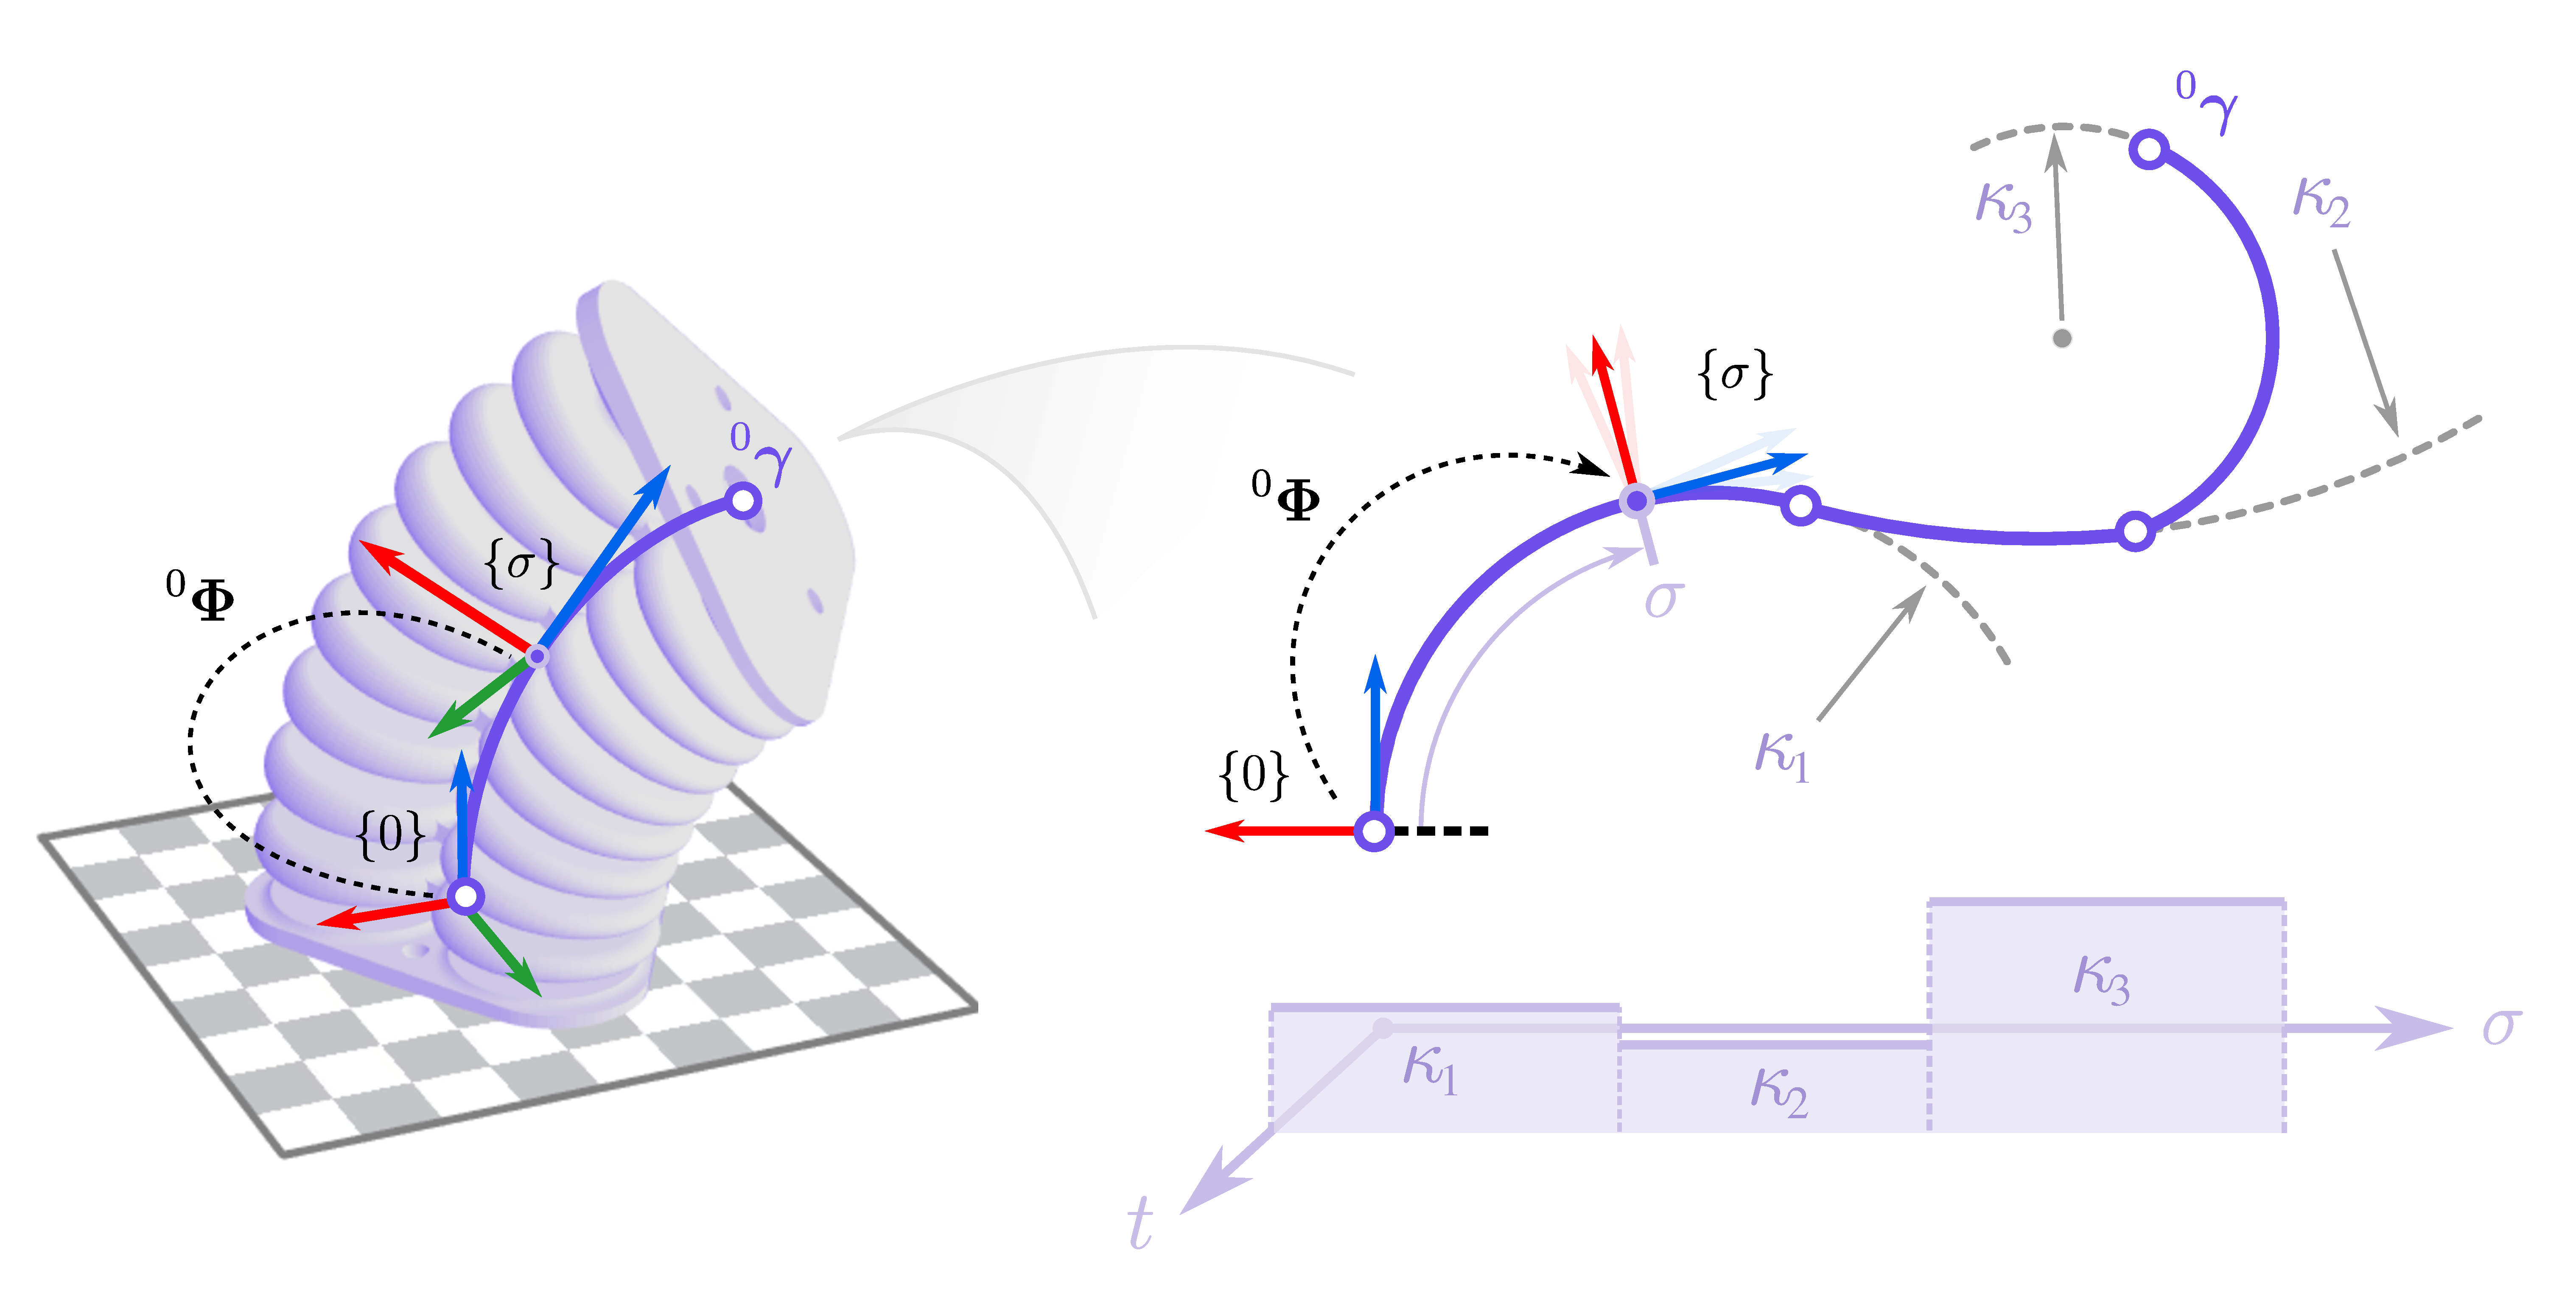
\includegraphics[width = 0.99\textwidth]{fig_C2_schematic.pdf}
  \caption{Schematic representation of the Piece-wise Constant Curvature (PCC) description for general soft \editl manipulator systems\editr, given by a parameterized curve $^0 \gammaB: \Xs \times \mathcal{Q} \to \R^3$ and orientation matrix $^0 \PhiB: \Xs \times \mathcal{Q} \to \SO{3}$. The frame $\{\sigma\}$ is an inertial coordinate frame that evolves over the backbone $^0 \gammaB$ such that variations in $\sigma$ give insight into its differential geometry.}
  \label{fig:C2:configuration}
\end{figure}
%
\begin{asm}[Piece-wise Constant Curvature]
\label{asm:C2:pcc}
Despite the inherent flexibility in soft robotics, it is sometimes sufficient to express the kinematics according to the \emph{Piecewise Constant Curvature} (PCC) condition. \editl This properties often originates from the "\textit{proper}" structural design of the soft robot, where parasitic motion is reduced by structural compliance \editr. Mathematically, it implies that the curvature of the continuous body satisfies $\kappa(\sigma_1,\q) = \kappa(\sigma_2,\q)$ for spatial coordinates on a local region on the soft manipulator $\sigma_1,\sigma_2 \subseteq \Xs$. As a result, this condition allows us to describe the full forward kinematics with a significantly reduced set of generalized coordinates, mitigating kinematic complexity in the model. Numerous works employ PCC models \cite{Falkenhahn2015,Katzschmann2019,Tatlicioglu2007,Marchese2016,Godage2016,DellaSantina2020a}, and depending on the elasticity \editl and structural geometry of the soft robot\editr, the PCC condition has been proven to be consistent for various soft robotic systems.
\end{asm}
%
{Following this Constant Curvature (CC) approach, we assign a coordinate frame that twists minimally along the backbone -- formally called the "\textit{Bishop frame}" (see \cite{Bishop1975}) -- parametrized by the following generalized coordinate vector:}
%
\begin{equation}
\vec{q} := \begin{pmatrix}
\,\varepsilon & \kappa_x & \kappa_y\,
\end{pmatrix}^\top \in \mathcal{Q},
\label{eq:C2:coordinate}
\end{equation}
%
\noindent where $\varepsilon_{-} \le \varepsilon \le \varepsilon_{+}$ is the elongation strain, and $\kappa_x,\,\kappa_y\in\mathbb{R}$ are the curvatures or angular strains in $x$-$z$ and $y$-$z$ plane, respectively; and $\mathcal{Q} \subset \R^3$ is an admissible space on which $\q$ evolves.\editl We will also introduce the following geometric variables\editr $\kappa = \inner{\kappa_x}{\kappa_y}$ and the curvature angle $\phi = \atantwo(\kappa_y,\kappa_x)$. It is worth mentioning that the joint description above is somewhat related to Renda. et al. \cite{Renda2018} who proposed a \emph{Piece-wise Constant Strain} (PCS) parametrization with the exception of including the twist along the tangent.

By exploring the differential geometry of the smooth backbone curve similar to Mochiyama et al. \cite{Mochiyama2003}, we can write the position vector $\gammaB(\sigma,\q)$ and the orientation matrix $\PhiB(\sigma,\q)$ for each material point $\sigma$ along the smooth backbone as a differential equation:
%
\begin{align}
\renewcommand*{\arraystretch}{2}{}
\frac{\partial \,\!\mat{\Phi}}{\partial \sigma}(\sigma,\q) & = \, \mat{\Phi}(\sigma,\vec{q}) \,\mat{\Gamma}^{\times} (\sigma,\q), \label{eq:C2:change_phi} \\[0.75em]
%
\frac{\partial \, \gammaB}{\partial \sigma}(\sigma,\q) & = \, \mat{\Phi}(\sigma,\vec{q}) \, \vec{U}(\sigma,\q), \label{eq:C2:change_p}
\end{align}
%
where \editl $\vec{\Gamma}^\times \in \sog{3}$ \editr is a skew-symmetric matrix composed of the entries of the vector $\vec{\Gamma} \in \R^3$, and $\vec{U}\in \R^3$ a vector representing the tangent along the extensible backbone. The skew-symmetric operator $(\,\cdot\,)^\times$ denotes the isomorphism between the Lie algebra $\sog{3}$ and $\R^3$. The vectors $\vec{\Gamma}$ and $\vec{U}$ are vectors that define the differential geometry of the backbone
\cite{Mochiyama2003} which are unique entries that live in the tangent space of the rigid-body transformation group (\ie, $T_{\SE{3}}$). Given the Bishop parametrization shown in \eqref{eq:C2:coordinate} and assuming the Piecewise Constant-Strain (PCC) condition, these geometric entities yield
%
\begin{align}
\vec{\Gamma}^\times(\sigma,t) & \simeq \vec{\Gamma}^\times(\sigma,\q(t)) \!\!\!\quad \xRightarrow[]{\textrm{\;\;PCC\;\;}}\quad \vec{\Gamma}^\times = \begin{pmatrix} 0 & 0 & \kappa_y \\ 0 & 0 & \kappa_x \\ -\kappa_y & -\kappa_x & 0 \end{pmatrix}, \label{eq:C2:Gamma}\\[0.35em]
%
\vec{U}(\sigma,t) & \simeq \vec{U}(\sigma,\q(t)) \!\quad \xRightarrow[]{\textrm{\;\;PCC\;\;}} \quad \;\; \vec{U} = \;\begin{pmatrix} \;0\;\;  &  \;0\;\; & \varepsilon + 1\ \end{pmatrix}^\top. \label{eq:C2:U}
\end{align}
%
%with $\vec{U}^\circ$ the unit-tangent pointing, and $\vec{\Gamma}^\circ$ the intrinsic curvature/torsion of the curve. For simplicity, lets assume $\vec{U}^\circ = (0,0,1)^\top$ and $\vec{\Gamma}^\circ = \vec{0}_3$.
Now, given an initial configuration of backbone's base, \ie, $\mat{\Phi}(0,\vec{q}) = \vec{\Phi}_0$ and $ \gammaB(0,\q) = \vec{0}_3$, we can now solve for the position and orientation for each material coordinate $\sigma$ along the backbone:
%
\begin{align}
\mat{\Phi}(\sigma,\vec{q}) & = \vec{\Phi}_0\exp_{\SO{3}}(\sigma \vec{\Gamma}^\times(\vec{q})), \label{eq:C2:phi_exact} \\[0.35em]
\gammaB(\sigma,\vec{q}) & = \int_0^\sigma\,^0\mat{\Phi}(s, \vec{q})\, \vec{U}(\vec{q}) \; ds,
\label{eq:C2:pos_exact}
\end{align}
%
where $\exp_{\SO{3}}: \sog{3} \to \SO{3}$ is the exponential map. Luckily, there exists a compact expression for the exponential mapping related to the orthogonal group of rotation matrices $\SO{3}$ called the "\emph{Rodriguez formulas}". \editl The rotation angle along the soft body can be computed by $\theta(\sigma,\q) := \int_0^\sigma \kappa(s,\q) \; ds = \kappa(\q) \sigma$. Notice that the rotation angle $\theta$ linearly depends on $\sigma$, which is a property that follows from Assumption \ref{asm:C2:pcc}. Then, given the expression for the angle of rotation, \editr we can compactly rewrite the rotation matrix \eqref{eq:C2:phi_exact} in terms of $\cos(\theta)$ and $\sin(\theta)$ using these formulas as follows \cite{Lynch2017}:
%
\begin{equation}
\PhiB(\theta) = \PhiB_0 \left( \mat{I}_3 + \left[ \frac{\sin(\theta)}{\theta} \right]  \GammaB^{\times} + \left[ \frac{1-\cos(\theta)}{\theta^2} \right]  \GammaB^{\times} \GammaB^{\times} \right).
\label{eq:C2:phi_rodr}
\end{equation}
%
Note that the closed-form solutions \eqref{eq:C2:phi_exact} and \eqref{eq:C2:pos_exact} represent the forward configuration kinematics of the backbone curve. To express the forward velocity kinematic, let
$\etaB(\sigma,\q,\dq) = \left( \vec{\omega}^\top, \vec{v}^\top \right)^\top \in \R^6 \cong \seg{3}$
 be the aggregate of the angular velocity and linear velocity components relative to an inertial frame at $\sigma$, where the space $\seg{3}$ denotes the Lie algebra of $\SE{3}$. The velocity twist is computed by the following integration procedure:
%
\begin{align}
 \etaB(\sigma,\q,\dq)& = \Ad_{\mat{g}(\sigma,\cdot)}\inv \int_0^\sigma \Ad_{\mat{g}(s,\cdot)}\, \JB^\star\! \dq\;ds, \notag \\ & 
 \,=:\, \JB(\q,\sigma) \dq, \label{eq:C2:vel_cont}
\end{align}
%
where $\Ad_g: \SE{3} \to \mathbb{R}^{6\times 6}$ denotes the adjoint transformation matrix regarding the rigid body transformation $\gB \in \SE{3}$ that maps local velocities (i.e., twist) to a frame located at $\sigma$, and $\JB^\star:\Q \to T_{\q}\Q$ the joint-axis matrix that relates the DOFs to the generalized coordinate description. Let it be clear that the joint-axis matrix is naturally constant for a soft segment modeled with the Constant-Strain (CS) assumption. We will later relax this assumption in Chapter 4. Nevertheless here, the joint-axis matrix for an extensible and bendable CS segment parametrized by the Bishop parameters is given by
%
\begin{align}
\renewcommand*{\arraystretch}{1}{}
\JB^\star := \begin{pmatrix}\dfrac{\p \GammaB}{\p \q}^\top & \dfrac{\p \UB}{\p \q}^\top \end{pmatrix}^\top  = \begin{pmatrix}
\,0 & 0 & 0 & 0 & 0 & 1 \, \\
\,0 & 1 & 0 & 0 & 0 & 0 \,  \\
\,-1 & 0 & 0 & 0 & 0 & 0 \,  \\
\end{pmatrix}^\top. \label{eq:C2:joint-axis-matrix}
\end{align}
%
Although we based the forward kinematics on Mochiyama et al. (2003, \cite{Mochiyama2003}), the derived expression for the velocity twist in \eqref{eq:C2:vel_cont} is analogous to the work of Renda et al. (2018, 2020; \cite{Renda2018,Renda2020}), and Boyer et al. (2010, 2021; \cite{Boyer2010,Boyer2021}). Please also note that
\eqref{eq:C2:vel_cont} gives rise to the geometric manipulator Jacobian $\JB(\sigma,\q)$ that defines the mapping from joint velocities to the velocity twist for a point $\sigma$ on the elastic body.

Given the explicit expression for the velocity twist in \eqref{eq:C2:vel_cont}, we can derive the acceleration twist \cite{Boyer2021,Mochiyama2003,Renda2018} which is obtained through time differentiation of \eqref{eq:C2:vel_cont}:
%
\begin{align}
\dot{\etaB}(\sigma,\q,\dq,\ddq) & = \JB \ddot{\q} + \Ad_{\gB(\cdot,\sigma)} \inv \int_0^\sigma \Ad_{\gB(s,\cdot)}
\ad_{\etaB(s,\cdot,\cdot)} \, \JB^\star\! \dq \;ds \notag \\
& :=  \JB(\sigma,\q)\ddot{\q} + \dmat{J}(\sigma,\q,\dot{\q}) \dot{\q},
\label{eq:C2:acceleration}
\end{align}
%
where $\ad_{\etaB}: \R^{6} \to \R^{6\times 6}$ denotes the adjoint transformation regarding the velocity twist $\vec{\etaB}^\wedge \in \seg{3}$. The reader is referred to Appendix \ref{app:C2:adjoint} for more detailed expressions on the adjoint transformations.
%
\begin{rmk}[Numerical instability near zero-curvature] For many of the PCC modeling frameworks \cite{Falkenhahn2015}, there are mentions of a\editl singularity point or discontinuity of the kinematic formulations at zero-curvature $\kappa = 0$. It is often reported that trajectories that pass through the origin lead to unbounded linear velocities $\vec{v} := \floor{\etaB}_3$, which may result in critical problems in practice. Although it is believed the problem is simply a by-product of the PCC hypothesis, this is however a common misconception, and it stems from a numerical origin.\editr To illustrate this, consider the inextensible planar case: $\varepsilon = \kappa_y = 0$ and $\kappa = \kappa_x$. \editl For simplicity, we assume $L = 1$.\editr Hence, by solving the forward kinematics for the position vector $\gammaB(\sigma,\kappa)$, and approaching zero-curvature from the positive domain $\kappa^{+} \to 0$, we see that
%
\begin{align}
\lim_{\kappa \to \,0^{+}}\gammaB(\sigma,\kappa) & = \begin{pmatrix} \dfrac{1-\cos(\sigma \kappa)}{\kappa}\,, & 0\,, & \dfrac{\sin(\sigma \kappa)}{\kappa} \end{pmatrix}^\top = \begin{pmatrix} 0 & 0 & \sigma \end{pmatrix}^\top,
\end{align}
%
so its limit clearly exists. Since the position vector $\gammaB$ is continuously differentiable when approaching the origin from both sides $\kappa \to 0^+$ and $\kappa \to 0^{-}$, it follows that $\dot{\gammaB}$ must be bounded for all $\kappa \in \Q$. We can simply check this by investigating the behavior of the linear-velocity components of the geometric Jacobian near zero-curvature, which yield
%
\begin{align}
\lim_{\kappa \to \,0^+} \floor{\JB}_3(\sigma,\kappa) & = \begin{pmatrix} \tfrac{\sigma \kappa \sin(\sigma \kappa) + 1 - \cos(\sigma \kappa)}{\kappa^2}\,, & 0\,, & \tfrac{\sigma \kappa \cos(\sigma \kappa) - \sin(\sigma \kappa) }{\kappa^2} \end{pmatrix}^\top \notag \\[0.35em] & = \begin{pmatrix} \sigma^2 & 0 & 0 \end{pmatrix}^\top.
\end{align}
%
\editl Again, its limit exists. Since both limits exist, we define $\vec{\gamma}(\sigma,0):= \lim_{\kappa \to \,0} \vec{\gamma}(\sigma,\kappa)$ and $\vec{J}(\sigma,0):= \lim_{\kappa \to \,0} \vec{J}(\sigma,\kappa)$. Consequently, the magnitude of the linear velocity of the end-effector reads simply $\lVert \dot{\gammaB}(L,\dot{\kappa}) \rVert = L^2\dot{\kappa} = L \omega_1$ with $\omega_1$ the angular velocity at the tip. Moreover, it is bounded for all $\kappa \in \mathcal{Q}$. This naturally poses an ambiguity on the origin of the kinematic singularity so often reported literature.\editr The problem is believed to be of numerical origin when considering the zero-division. To make matters worse, deriving analytical expressions for accelerations will contain similar expressions that are hard to stabilize numerically. To resolve this issue, we opt for a numerical approximation of the forward kinematics -- namely, we employ an explicit forward integration scheme (\ie, trapezoidal integration) to solve \eqref{eq:C2:change_phi} and \eqref{eq:C2:change_p}.
\end{rmk}

\begin{figure}[!h]
  % This file was created by matlab2tikz.
%
%The latest updates can be retrieved from
%  http://www.mathworks.com/matlabcentral/fileexchange/22022-matlab2tikz-matlab2tikz
%where you can also make suggestions and rate matlab2tikz.
%
\definecolor{mycolor1}{rgb}{0.06275,0.35686,0.84706}%
\definecolor{mycolor2}{rgb}{0.86667,0.21176,0.10980}%
\definecolor{mycolor3}{rgb}{0.18039,0.52157,0.25098}%
%
\begin{tikzpicture}

\begin{axis}[%
width=0.259\textwidth,
height=0.215\textwidth,
at={(0\textwidth,0\textwidth)},
scale only axis,
xmin=0,
xmax=5.01,
xlabel style={font=\color{white!15!black}},
xlabel={time (s)},
ymin=-2,
ymax=2,
ylabel style={font=\color{white!15!black}},
ylabel={$\q_d$},
axis background/.style={fill=white},
xmajorgrids,
ymajorgrids,
ylabel style={yshift=-9.5pt}
]
\addplot [color=mycolor1, line width=1.5pt, forget plot]
  table[row sep=crcr]{%
0	0\\
0.0590118023604722	0.0122599350151695\\
0.122024404880976	0.051245683586683\\
0.197039407881577	0.127356433673519\\
0.306061212242448	0.274610958461174\\
0.464092818563713	0.485281744378211\\
0.539107821564313	0.550009396707688\\
0.599119823964793	0.574155119595387\\
0.654130826165233	0.570918154822998\\
0.708141628325666	0.542425923995588\\
0.766153230646129	0.483585222567674\\
0.833166633326665	0.381001848782168\\
0.914182836567313	0.214127314579629\\
1.02820564112823	-0.075581754600881\\
1.25925185037007	-0.672851821290417\\
1.34526905381076	-0.833669846120815\\
1.41328265653131	-0.919160442883364\\
1.47129425885177	-0.95862945224353\\
1.52230446089218	-0.966293478371877\\
1.57331466293259	-0.948199994340202\\
1.62732546509302	-0.90137626204806\\
1.68933786757351	-0.814258548692571\\
1.76335267053411	-0.668276174824877\\
1.85537107421484	-0.435076623934572\\
1.99539907981596	-0.0143847160291388\\
2.19043808761752	0.562122882172909\\
2.28645729145829	0.78232701823107\\
2.36147229445889	0.906026029952742\\
2.4244848969794	0.971401468926922\\
2.47949589917984	0.997472999626086\\
2.53050610122024	0.995067322990411\\
2.58251650330066	0.966335526484759\\
2.63952790558112	0.905286120543856\\
2.70554110822164	0.798558894400302\\
2.78455691138228	0.62627694206536\\
2.8875775155031	0.345873241993202\\
3.26665333066613	-0.743113935603639\\
3.34566913382677	-0.884745361525436\\
3.41068213642729	-0.960888000773404\\
3.46669333866773	-0.994529710207253\\
3.51770354070814	-0.998453103672079\\
3.56871374274855	-0.976789847418135\\
3.624724944989	-0.924209595097784\\
3.68873774754951	-0.829302846512608\\
3.76375275055011	-0.675905403764888\\
3.85977195439088	-0.426427403766472\\
4.0128025605121	0.0402095863869585\\
4.1878375675135	0.556451691884553\\
4.28385677135427	0.778179781889043\\
4.35987197439488	0.904655728387877\\
4.42288457691538	0.970797027717512\\
4.47789557911582	0.997589797446857\\
4.52790558111622	0.996159624088327\\
4.57991598319664	0.968648768140962\\
4.6369273854771	0.908894839975858\\
4.70294058811762	0.803552513256307\\
4.78195639127826	0.632676263537522\\
4.88397679535907	0.356479989904654\\
5	8.88178419700125e-16\\
};
\addplot [color=mycolor2, line width=1.5pt, forget plot]
  table[row sep=crcr]{%
0	0\\
0.138027605521104	0.140440300108925\\
0.211042208441689	0.184935584810103\\
0.272054410882176	0.196656209080302\\
0.329065813162632	0.183310753811706\\
0.388077615523104	0.143577314476932\\
0.454090818163633	0.0688810755447316\\
0.533106621324265	-0.0570083146317186\\
0.645129025805161	-0.281096403013078\\
0.835167033406681	-0.662476511437434\\
0.916183236647329	-0.777169753245791\\
0.980196039207842	-0.832701926306017\\
1.03520704140828	-0.851571468783066\\
1.08621724344869	-0.843577250292476\\
1.13922784556911	-0.808789721087341\\
1.19823964792959	-0.739024227249642\\
1.26625325065013	-0.620955121877476\\
1.3502700540108	-0.427767812642783\\
1.46629325865173	-0.101666846450176\\
1.72234446889378	0.633525295214997\\
1.81136227245449	0.820837424693816\\
1.88337667533507	0.92640916650209\\
1.94338867773555	0.978331555991308\\
1.99639927985597	0.99518363496166\\
2.04740948189638	0.985184790347176\\
2.1004200840168	0.947820917223337\\
2.15943188637728	0.875183689696618\\
2.22844568913783	0.752107632272527\\
2.31346269253851	0.552461842844861\\
2.42848569713943	0.222651201302659\\
2.71854370874175	-0.633815634394776\\
2.80756151230246	-0.822691363947944\\
2.87857571514303	-0.928076540294048\\
2.93858771754351	-0.981414393680224\\
2.99159831966393	-0.999628398951698\\
3.04260852170434	-0.991037597553407\\
3.09561912382476	-0.955207840530338\\
3.15463092618524	-0.884300387785018\\
3.22364472894579	-0.7631603021345\\
3.30766153230646	-0.568142665295742\\
3.42068413682737	-0.246607234578534\\
3.72574514902981	0.65122625379941\\
3.8127625525105	0.831927524141501\\
3.88377675535107	0.93407870842546\\
3.94278855771154	0.983891068491499\\
3.99579915983197	0.999912900564358\\
4.04680936187237	0.989206735619766\\
4.0998199639928	0.951231137729379\\
4.15983196639328	0.876560868859253\\
4.22984596919384	0.750430990306204\\
4.31586317263453	0.546754312000056\\
4.43288657731546	0.209284340535875\\
4.71394278855771	-0.622647147364128\\
4.80396079215843	-0.816268101959198\\
4.87597519503901	-0.925047608943518\\
4.9369873974795	-0.980469837601955\\
4.98999799959992	-0.999506362945193\\
5	-0.999999999998463\\
};
\addplot [color=mycolor3, line width=1.5pt, forget plot]
  table[row sep=crcr]{%
0	-0\\
0.0590118023604722	-0.0323127302272486\\
0.108021604320864	-0.0331290824818566\\
0.157031406281257	-0.0079769875375062\\
0.212042408481697	0.0500216589361884\\
0.283056611322264	0.162185680095956\\
0.485097019403881	0.506055784611869\\
0.536107221444289	0.543684543712172\\
0.578115623124625	0.547118496091529\\
0.619123824764953	0.523782154432988\\
0.664132826565313	0.466781106891244\\
0.718143628725745	0.35651568991531\\
0.785157031406281	0.165020918099894\\
0.890178035607121	-0.209610885997843\\
1.02020404080816	-0.656165846278042\\
1.08621724344869	-0.813331876653166\\
1.13622724544909	-0.8827564770361\\
1.17623524704941	-0.902858557904033\\
1.21324264852971	-0.891876333186355\\
1.25225045009002	-0.849343403567872\\
1.29825965193039	-0.75980970794915\\
1.35527105421084	-0.595513228979666\\
1.43128625725145	-0.304509569554719\\
1.70234046809362	0.802351589692006\\
1.75935187037407	0.927771606903312\\
1.80436087217443	0.980075766519771\\
1.84136827365473	0.990077945444886\\
1.87737547509502	0.970779584879269\\
1.91838367673535	0.914613712496442\\
1.96739347869574	0.80264348414426\\
2.02940588117624	0.600183129717624\\
2.11542308461692	0.238476117081353\\
2.33046609321864	-0.696803833599685\\
2.39647929585917	-0.882732768124136\\
2.44748949789958	-0.969018921052845\\
2.4874974994999	-0.997830617495056\\
2.52250450090018	-0.994023401063271\\
2.55951190238048	-0.960649427962859\\
2.60252050410082	-0.885345365627133\\
2.65653130626125	-0.73993292743766\\
2.72654530906181	-0.482199139020603\\
2.83856771354271	0.0246624641119846\\
2.97559511902381	0.621277881997434\\
3.04660932186437	0.844169225727331\\
3.1006201240248	0.951944439490648\\
3.14362872574515	0.994104036503082\\
3.17963592718544	0.998126097022847\\
3.21564312862573	0.973479302424193\\
3.25665133026605	0.911429266327099\\
3.30666133226645	0.79016811146077\\
3.37067413482697	0.572402197653537\\
3.4626925385077	0.174902851173357\\
3.65173034606921	-0.655626629756043\\
3.72074414882977	-0.862521673164816\\
3.77275455091018	-0.959529089678471\\
3.81476295259052	-0.996173299612285\\
3.85077015403081	-0.996625968608955\\
3.8877775555111	-0.96726798143933\\
3.93078615723145	-0.896391559355475\\
3.98279655931186	-0.76204628869428\\
4.0498099619924	-0.523261917173079\\
4.15183036607321	-0.0698574757930102\\
4.30986197239448	0.62473490045429\\
4.38087617523505	0.846533085581687\\
4.43488697739548	0.953293435683277\\
4.47789557911582	0.994579768326681\\
4.51390278055611	0.997854639446826\\
4.55091018203641	0.971359701253584\\
4.59291858371674	0.905657492920928\\
4.64392878575715	0.778672904138067\\
4.70994198839768	0.549251284827934\\
4.80596119223845	0.128630790373577\\
4.97999599919984	-0.637409462896398\\
5	-0.707106781185458\\
};
\end{axis}

\begin{axis}[%
width=0.259\textwidth,
height=0.215\textwidth,
at={(0.341\textwidth,0\textwidth)},
scale only axis,
xmin=0,
xmax=5.01,
xlabel style={font=\color{white!15!black}},
xlabel={time (s)},
ymin=-6,
ymax=6,
ylabel style={font=\color{white!15!black}},
ylabel={$\dq_d$},
axis background/.style={fill=white},
xmajorgrids,
ymajorgrids,
ylabel style={yshift=-9.5pt}
]
\addplot [color=mycolor1, line width=1.5pt, forget plot]
  table[row sep=crcr]{%
0	0.00354490068904045\\
0.137027405481096	0.903588308385592\\
0.206041208241649	1.22856452598255\\
0.257051410282056	1.38060740669893\\
0.296059211842368	1.43857878332504\\
0.326065213042608	1.44671619310838\\
0.356071214242848	1.42249130990263\\
0.39007801560312	1.3560092907744\\
0.432086417283457	1.21821465698646\\
0.485097019403881	0.962586034545687\\
0.553110622124425	0.520529889641796\\
0.651130226045209	-0.270803972466815\\
0.857171434286857	-1.96111846971092\\
0.93118623724745	-2.39268873749415\\
0.988197639527906	-2.61578401240715\\
1.03220644128826	-2.71435218975166\\
1.06621324264853	-2.74427973959115\\
1.09621924384877	-2.73665215168262\\
1.12822564512903	-2.69342117279692\\
1.16623324664933	-2.59588760182128\\
1.21324264852971	-2.40873834185884\\
1.27225445089018	-2.07805095116542\\
1.34626925385077	-1.53498416704634\\
1.44928985797159	-0.609800554006279\\
1.7373474694939	2.06478538831989\\
1.81936387277455	2.60307834026396\\
1.88337667533507	2.90062171255517\\
1.93538707741548	3.05371910764113\\
1.97639527905581	3.11545185690039\\
2.00840168033607	3.12679834073453\\
2.03940788157632	3.10692697008051\\
2.0744148829766	3.04832587668127\\
2.11742348469694	2.92503238525876\\
2.16943388677736	2.70379607461824\\
2.23344668933787	2.33206311088885\\
2.31346269253851	1.73595350618949\\
2.42348469693939	0.745755428207096\\
2.72054410882176	-2.00968788046552\\
2.80556111222244	-2.57586752681016\\
2.87157431486297	-2.89102311132145\\
2.9245849169834	-3.05482622701098\\
2.96659331866373	-3.12471640436199\\
2.999599919984	-3.14152189462515\\
3.03060612122425	-3.12655715277568\\
3.06461292258452	-3.0760658872595\\
3.10662132426485	-2.96535682645882\\
3.15663132626525	-2.76652815312306\\
3.21864372874575	-2.42602567294836\\
3.29565913182637	-1.8771253886638\\
3.39767953590718	-0.987885846273739\\
3.75075015003001	2.23014715782088\\
3.82876575315063	2.70040323156362\\
3.89077815563113	2.96011198400992\\
3.93978795759152	3.08647630578385\\
3.97879575915183	3.13494797811861\\
4.01080216043209	3.1396111777881\\
4.04280856171234	3.11255800697227\\
4.07981596319264	3.04211546348687\\
4.124824964993	2.90122307727425\\
4.17983596719344	2.65075511896351\\
4.24684936987398	2.23986170977253\\
4.33186637327465	1.57905334730502\\
4.45289057811562	0.458374253608507\\
4.69693938787758	-1.82607588925665\\
4.7869573914783	-2.46688451700194\\
4.85697139427886	-2.83188138573282\\
4.9129825965193	-3.02625903108539\\
4.95799159831966	-3.11491811053946\\
4.99299859971994	-3.14093609486879\\
5	-3.14158748587636\\
};
\addplot [color=mycolor2, line width=1.5pt, forget plot]
  table[row sep=crcr]{%
0	1.12837322264768\\
0.0290058011602321	1.11287690718957\\
0.0620124024804962	1.05918703548886\\
0.103020604120824	0.940995733860333\\
0.154030806161233	0.720852429683366\\
0.221044208841769	0.329040615346998\\
0.324064812962592	-0.415015201309904\\
0.479095819163833	-1.51762477223098\\
0.550110022004401	-1.88091677154614\\
0.603120624124825	-2.05657754379251\\
0.643128625725145	-2.12690523971632\\
0.674134826965394	-2.14233493262017\\
0.703140628125626	-2.12518565975495\\
0.736147229445889	-2.06847786435016\\
0.776155231046209	-1.94764697173144\\
0.826165233046609	-1.72032118445276\\
0.888177635527105	-1.33287793109094\\
0.970194038807762	-0.677703297361942\\
1.1122224444889	0.656669942201704\\
1.25425085017003	1.92027334813605\\
1.33826765353071	2.4957239295581\\
1.40328065613123	2.8110209600663\\
1.45429085817163	2.96740997845937\\
1.49429885977195	3.03077028972536\\
1.52630526105221	3.04316268415615\\
1.55631126225245	3.0238292307504\\
1.59131826365273	2.96385353194767\\
1.63332666533307	2.84010088177006\\
1.68533706741348	2.61261209274866\\
1.74934986997399	2.23016785497343\\
1.83036607321464	1.61058449856721\\
1.94538907781556	0.55355301879334\\
2.20544108821764	-1.88333064164048\\
2.29345869173835	-2.49961881538618\\
2.3624724944989	-2.85081712197516\\
2.41748349669934	-3.03514561937135\\
2.46149229845969	-3.11735537496245\\
2.49549909981996	-3.14000923889623\\
2.52650530106021	-3.12935139813733\\
2.56051210242048	-3.08346030159967\\
2.6005201040208	-2.9844099202232\\
2.6505301060212	-2.79450937790965\\
2.71154230846169	-2.47007506810393\\
2.78655731146229	-1.94858631705674\\
2.88457691538308	-1.10996961666554\\
3.10262052410482	0.99996718143458\\
3.22164432886577	2.01874975626282\\
3.30566113222645	2.57684537272085\\
3.37167433486697	2.89165495774407\\
3.4246849369874	3.05520852382526\\
3.46669333866773	3.12491681950401\\
3.499699939988	3.14158841415858\\
3.53070614122825	3.12650471358071\\
3.56471294258852	3.07589032073885\\
3.60672134426885	2.96503961364553\\
3.65673134626925	2.76605754535741\\
3.71874374874975	2.42538893386612\\
3.79575915183037	1.87632266950521\\
3.89777955591118	0.986940126259217\\
4.25085017003401	-2.23084317749245\\
4.32886577315463	-2.70090796640865\\
4.39087817563513	-2.96044270093426\\
4.43988797759552	-3.08666036495903\\
4.47889577915583	-3.13501205318945\\
4.51090218043609	-3.13957601885231\\
4.54290858171634	-3.11242397791472\\
4.57991598319664	-3.04186887567698\\
4.624924984997	-2.9008442325007\\
4.67993598719744	-2.65022515672919\\
4.74694938987798	-2.23916940295443\\
4.83196639327866	-1.57819986384533\\
4.95299059811962	-0.457397634949563\\
5	0.00493479812624376\\
};
\addplot [color=mycolor3, line width=1.5pt, forget plot]
  table[row sep=crcr]{%
0	-0.794115508462454\\
0.0580116023204642	-0.277364611734568\\
0.26505301060212	1.70491593082617\\
0.306061212242448	1.87842338112035\\
0.334066813362672	1.92300384411942\\
0.356071214242848	1.91292691038186\\
0.38007601520304	1.85542433262415\\
0.411082216443289	1.70919219099674\\
0.451090218043609	1.40465740373763\\
0.504100820164033	0.820935563376146\\
0.578115623124625	-0.248600075058891\\
0.762152430486097	-2.99671953899652\\
0.816163232646529	-3.4867860854134\\
0.855171034206841	-3.68308225183768\\
0.882176435287057	-3.73307210749446\\
0.902180436087217	-3.72294329754286\\
0.924184836967394	-3.66485742913014\\
0.954190838167634	-3.50676773602809\\
0.993198639727946	-3.16939676216821\\
1.04320864172835	-2.53683562435458\\
1.11022204440888	-1.40251215395337\\
1.23224644928986	1.09146932720294\\
1.34026805361072	3.11962860739989\\
1.40428085617123	3.97847580467464\\
1.45229045809162	4.38259317834563\\
1.4872974594919	4.53109137402165\\
1.51030206041208	4.55856842712607\\
1.53030606121224	4.53675451436047\\
1.55431086217243	4.45469330662973\\
1.58631726345269	4.25233666981845\\
1.62832566513303	3.83346415954477\\
1.68233646729346	3.06612040251519\\
1.75535107021404	1.70902193090805\\
2.03440688137628	-3.80704018778977\\
2.08841768353671	-4.38067909824091\\
2.12942588517704	-4.62780828971085\\
2.15843168633727	-4.6982027777484\\
2.17843568713743	-4.69538596539201\\
2.1994398879776	-4.64729630338051\\
2.22744548909782	-4.5121578146679\\
2.26445289057812	-4.21315733318806\\
2.3124624924985	-3.63571053810641\\
2.374474894979	-2.61980512471882\\
2.46549309861972	-0.754128407877475\\
2.6495299059812	3.05964290826855\\
2.71654330866173	4.02147655398821\\
2.76655331066213	4.48381747958504\\
2.80356071214243	4.66721925102645\\
2.82956591318264	4.71152470359658\\
2.84856971394279	4.69919553002523\\
2.87157431486297	4.63390058682298\\
2.90158031606321	4.46715113358115\\
2.94058811762353	4.11776373765277\\
2.99059811962393	3.4689862272862\\
3.05761152230446	2.30691776642933\\
3.16363272654531	0.0563190270418401\\
3.30666133226645	-2.89690138385146\\
3.37667533506701	-3.9448221542987\\
3.42868573714743	-4.45241981565303\\
3.46769353870774	-4.65954561876156\\
3.49469893978796	-4.71117486462973\\
3.51470294058812	-4.70029361858979\\
3.53670734146829	-4.64013279511158\\
3.56671334266853	-4.47797683817697\\
3.60572114422885	-4.13425107699655\\
3.65573114622925	-3.49192821143007\\
3.72174434886977	-2.35576737664234\\
3.82576515303061	-0.156931641015601\\
3.97379475895179	2.90509369151093\\
4.04380876175235	3.950496362776\\
4.09581916383277	4.45581244484655\\
4.13482696539308	4.66108744519533\\
4.16183236647329	4.71140168604915\\
4.18183636727345	4.69954306835578\\
4.20484096819364	4.63434132500523\\
4.23484696939388	4.46772453283112\\
4.27385477095419	4.11851887812703\\
4.32386477295459	3.46996990086312\\
4.39087817563513	2.30815865696121\\
4.49689937987598	0.0577494594312666\\
4.63992798559712	-2.89575760597693\\
4.70994198839768	-3.94402589682519\\
4.7619523904781	-4.45194298479568\\
4.80096019203841	-4.65932964437099\\
4.82796559311862	-4.71114488543943\\
4.84796959391878	-4.70040215831249\\
4.86997399479896	-4.64039276611033\\
4.8999799959992	-4.47843880303433\\
4.93898779755951	-4.13496168317129\\
4.98899779955991	-3.49292197179463\\
5	-3.32429866327344\\
};
\end{axis}

\begin{axis}[%
width=0.259\textwidth,
height=0.215\textwidth,
at={(0.682\textwidth,0\textwidth)},
scale only axis,
xmin=0,
xmax=5.01,
xlabel style={font=\color{white!15!black}},
xlabel={time (s)},
ymin=-30,
ymax=30,
ylabel style={font=\color{white!15!black}},
ylabel={$\ddq_d$},
axis background/.style={fill=white},
xmajorgrids,
ymajorgrids,
ylabel style={yshift=-9.5pt}
]
\addplot [color=mycolor1, line width=1.5pt, forget plot]
  table[row sep=crcr]{%
0	7.08971722508816\\
0.0170034006801352	7.06254176227866\\
0.0380076015203041	6.96211357748433\\
0.0670134026805353	6.70383363218785\\
0.105021004200839	6.16331809076554\\
0.15503100620124	5.13123086154366\\
0.221044208841768	3.30313004756611\\
0.322064412882577	-0.140715150531712\\
0.483096619323865	-5.57492932673487\\
0.555111022204441	-7.34242512612227\\
0.609121824364873	-8.2298345369658\\
0.650130026005201	-8.61942170460317\\
0.679135827165434	-8.74010611151554\\
0.696139227845569	-8.75056964311227\\
0.714142828565713	-8.71323899853671\\
0.738147629525905	-8.58686459570546\\
0.770154030806161	-8.28547401565682\\
0.812162432486497	-7.67074463808859\\
0.866173234646929	-6.54917377090891\\
0.937187437487498	-4.60734590265721\\
1.04320864172835	-1.07483524322571\\
1.24624924984997	5.72961331213317\\
1.32926585317063	7.81639650559995\\
1.39427885577116	8.9859331390274\\
1.44528905781156	9.58253887084481\\
1.48529705941188	9.8442837551671\\
1.51330266053211	9.91865276034343\\
1.53230646129226	9.91831589369774\\
1.55331066213243	9.87066630009359\\
1.58031606321264	9.73764473499728\\
1.61632326465293	9.43822354992907\\
1.6623324664933	8.86253703324957\\
1.72034406881376	7.8537245560284\\
1.79335867173435	6.19915830635254\\
1.89137827565513	3.47504190478798\\
2.25345069013803	-7.05759085861679\\
2.32946589317864	-8.49825043913732\\
2.39047809561912	-9.30375995789046\\
2.4374874974995	-9.69098733938356\\
2.47349469893979	-9.84429919326235\\
2.49849969993999	-9.87645177319418\\
2.51850370074015	-9.85815891485498\\
2.54250850170034	-9.78470810142351\\
2.5745149029806	-9.6001934501988\\
2.61552310462092	-9.22223443122761\\
2.66653330666133	-8.53959500779489\\
2.72954590918184	-7.39663922633138\\
2.80856171234247	-5.56189473532864\\
2.91558311662332	-2.55857583281172\\
3.22764552910582	6.49527125262672\\
3.30966193238648	8.17448519252473\\
3.374674934987	9.12633838257015\\
3.42568513702741	9.60899637547641\\
3.46469293858772	9.81236106656347\\
3.49269853970794	9.86769341093652\\
3.5127025405081	9.86048208595491\\
3.53570714142829	9.80407057871169\\
3.56471294258852	9.66005045055507\\
3.60272054410882	9.35027485493567\\
3.65073014602921	8.7694054033971\\
3.70974194838968	7.78440013127213\\
3.78275655131026	6.20094073200406\\
3.87877575515103	3.63970724426288\\
4.05881176235247	-1.84364405983484\\
4.19783956791358	-5.77205567675598\\
4.2868573714743	-7.75761622429094\\
4.35587117423485	-8.88854079805768\\
4.41088217643529	-9.49382693860024\\
4.45389077815563	-9.77065608576133\\
4.48489697939588	-9.85991079216486\\
4.50590118023605	-9.86727677343424\\
4.52690538107622	-9.83169388013572\\
4.55391078215643	-9.72310658142739\\
4.58891778355671	-9.47842189369386\\
4.63392678535707	-8.99611634308517\\
4.68893778755751	-8.16403545489397\\
4.75695139027806	-6.80236720584926\\
4.84396879375875	-4.61913345423115\\
4.97299459891978	-0.805433305647973\\
5	0.0310062018553658\\
};
\addplot [color=mycolor2, line width=1.5pt, forget plot]
  table[row sep=crcr]{%
0	-0.0356665298542058\\
0.14002800560112	-4.67099677947669\\
0.210042008401681	-6.35787080027761\\
0.262052410482097	-7.18121414389206\\
0.301060212042408	-7.52419844540775\\
0.328065613122625	-7.61679085886646\\
0.34506901380276	-7.61344158614619\\
0.364072814562913	-7.55338671970529\\
0.390078015603121	-7.3759254387018\\
0.425085017003401	-6.96795293714247\\
0.47009401880376	-6.17536023821841\\
0.528105621124224	-4.76203193936642\\
0.608121624324864	-2.2616035058598\\
0.90118023604721	7.41655342073599\\
0.965193038607721	8.68477119764233\\
1.01520304060812	9.31550428917571\\
1.05321064212843	9.57115136568376\\
1.07921584316863	9.63325353187106\\
1.09821964392879	9.62095442347266\\
1.12022404480896	9.54664003094408\\
1.14922984596919	9.35230091148043\\
1.1872374474895	8.93817915492701\\
1.23624724944989	8.15570308454472\\
1.29825965193039	6.81305056038362\\
1.38127625525105	4.53205984490834\\
1.51730346069214	0.137104630163254\\
1.6873374674935	-5.19413042832095\\
1.77835567113423	-7.44111083206267\\
1.8493698739748	-8.73764863851267\\
1.90638127625525	-9.44363453025954\\
1.95139027805561	-9.77614657982073\\
1.98439687937588	-9.89060722533797\\
2.00640128025605	-9.90571841918975\\
2.02640528105621	-9.87708129185361\\
2.05241048209642	-9.77998577411654\\
2.08541708341668	-9.56077689839852\\
2.12842568513703	-9.11882330623115\\
2.18143628725745	-8.34382797509914\\
2.24744948989798	-7.05721408722493\\
2.33146629325865	-4.99130619335819\\
2.45249049809962	-1.45521934033521\\
2.69453890778156	5.68634972386572\\
2.78455691138228	7.71289662082619\\
2.85457091418284	8.87123751025509\\
2.90958191638328	9.48327346161904\\
2.95259051810362	9.76549714637454\\
2.98459691938388	9.86011816772603\\
3.00560112022404	9.86808705516484\\
3.02660532106421	9.83309714619462\\
3.05361072214443	9.72525700271287\\
3.08861772354471	9.48151268853614\\
3.13262652530506	9.01304744316267\\
3.1876375275055	8.18694988291568\\
3.25565113022605	6.83174606330716\\
3.34266853370674	4.65484935746607\\
3.47069413882777	0.876546802294875\\
3.6877375475095	-5.51511477797639\\
3.77975595119024	-7.61957450245987\\
3.85077015403081	-8.81865742330401\\
3.90678135627125	-9.45828980758456\\
3.95079015803161	-9.75661509139414\\
3.98279655931186	-9.85681253462545\\
4.00480096019204	-9.86795820689945\\
4.02580516103221	-9.8346227153101\\
4.05281056211242	-9.72890484618461\\
4.0868173634727	-9.4963693895167\\
4.13082616523305	-9.03523157269603\\
4.18483696739348	-8.23480517953001\\
4.25185037007402	-6.91608604630467\\
4.33686737347469	-4.81255275530668\\
4.46089217843569	-1.17876018750085\\
4.69093818763753	5.59713704895159\\
4.78195639127826	7.66275629837665\\
4.85197039407882	8.8353040648137\\
4.90798159631926	9.46885282937515\\
4.95199039807962	9.76215955428295\\
4.98399679935987	9.85863512259488\\
5	9.86954757942193\\
};
\addplot [color=mycolor3, line width=1.5pt, forget plot]
  table[row sep=crcr]{%
0	7.5744225756329\\
0.0520104020804162	9.85795253565652\\
0.0890178035607114	10.7343646901029\\
0.113022604520904	10.9368263420187\\
0.126025205041007	10.9227666810555\\
0.142028405681135	10.7856109086146\\
0.16503300660132	10.3588706857098\\
0.197039407881576	9.32929431048124\\
0.240048009601921	7.21344321073802\\
0.300060012002401	3.12899615273476\\
0.541108221644329	-14.5767064028135\\
0.583116623324663	-15.8947102220086\\
0.611122224444888	-16.2686397032763\\
0.622124424884976	-16.3000792190449\\
0.634126825365072	-16.2590964666309\\
0.651130226045208	-16.0662320020655\\
0.67613522704541	-15.4974275623498\\
0.710142028405681	-14.1945663307275\\
0.75515103020604	-11.6027109979822\\
0.816163232646531	-6.78180501212378\\
0.918183636727345	3.19925678471389\\
1.0372074414883	14.2630289394763\\
1.1002200440088	18.3769434543013\\
1.14622924584917	20.2284519962292\\
1.17923584716943	20.8825917599187\\
1.19923984796959	20.9940018330856\\
1.21024204840968	20.9627983709382\\
1.22624524904981	20.8005305254444\\
1.25025005001	20.300173284471\\
1.28325665133027	19.1232943641539\\
1.32726545309062	16.7321518603769\\
1.38527705541108	12.3448435289664\\
1.46929385877175	4.24762456605077\\
1.66433286657331	-15.006835410114\\
1.72834566913383	-19.2314865141707\\
1.77635527105421	-21.2288700042196\\
1.81136227245449	-21.9820872663368\\
1.83336667333467	-22.1406342791886\\
1.84536907381476	-22.1238119583189\\
1.86137227445489	-21.9881962890689\\
1.88437687537508	-21.5687174401902\\
1.91638327665533	-20.5551161436279\\
1.95839167833567	-18.5063456770163\\
2.01340268053611	-14.7274455786217\\
2.08841768353671	-8.02930998083884\\
2.35847169433887	17.4889091607566\\
2.41448289657932	20.4580950794453\\
2.45649129825965	21.7593237376024\\
2.48549709941988	22.1621020797258\\
2.49949989997999	22.2084088691288\\
2.51150230046009	22.1710021117705\\
2.52850570114023	21.9964824567098\\
2.55351070214043	21.4835583106643\\
2.5875175035007	20.3092524488913\\
2.63252650530106	17.9608482179239\\
2.69053810762152	13.7652243370479\\
2.77155431086217	6.27861523427864\\
3.00360072014403	-16.0384936526148\\
3.06461292258452	-19.7357108331353\\
3.11062212442489	-21.463698030133\\
3.14362872574515	-22.0870363960568\\
3.16463292658532	-22.2064523468513\\
3.17663532706541	-22.1770731289039\\
3.19263852770554	-22.0276153410914\\
3.21664332866573	-21.5691020724051\\
3.249649929986	-20.4902631329995\\
3.29265853170634	-18.3476492789936\\
3.34866973394679	-14.44841849918\\
3.4256851370274	-7.52047923802124\\
3.68573714742949	17.1151521202173\\
3.74374874974995	20.2996418279255\\
3.78675735147029	21.6963760554245\\
3.81676335267053	22.146824126934\\
3.83276655331066	22.2065248116632\\
3.84476895379076	22.1684518725285\\
3.86177235447089	21.9932254539312\\
3.88677735547109	21.479711348027\\
3.92078415683137	20.3053143584819\\
3.96579315863173	17.9577095353878\\
4.02380476095219	13.7639924762123\\
4.10482096419284	6.28037173283591\\
4.3368673734747	-16.0343061430535\\
4.39787957591518	-19.7326927237063\\
4.44388877775555	-21.4618857962146\\
4.47689537907582	-22.0862019015833\\
4.49789957991598	-22.2062702477377\\
4.50990198039608	-22.1772700763623\\
4.52590518103621	-22.0283212123418\\
4.5499099819964	-21.5705710293612\\
4.58291658331666	-20.4927599587457\\
4.62592518503701	-18.3514020697384\\
4.68193638727746	-14.4535738878515\\
4.75895179035807	-7.52695343386733\\
5	15.7762366578273\\
};
\end{axis}
\end{tikzpicture}%
  \vspace{-5mm}
  \caption{The time evolution of the predefined geometric strain parameters of the Piece-wise Constant curvature model $\q_d \to  (\varepsilon, \, \kappa_x,\,\kappa_y)^\top$ and their corresponding time-derivatives $\dq_d$ and $\ddq_d$, given by the (spatially constant) elongation $\varepsilon$ \data{Matlab1}, and the \editl (spatially constant)\editr curvatures $\kappa_x$ \data{Matlab2} and $\kappa_y$ \data{Matlab3}.}
  \label{fig:C2:EX1:strain_ref}
\end{figure}

\begin{example}[Kinematic behavior of PCC segment]
As an illustrative example, we perform a numerical simulation of the forward kinematics for a single PCC segment.\editl We select a differentiable reference trajectory $\q(t) \equiv \q_d(t)$, $\dot{\q}(t) \equiv \dot{\q}_d(t)$ and $\ddot{\q}(t) \equiv \ddot{\q}_d(t)$ that passes the zero-curvature point  given by \editr:
%
\begin{align*}
\q_d(t) &  =  \erf(t) \cdot \begin{pmatrix} \varepsilon_0 \sin(\omega t) & \kappa_0 \cos(\omega t) & \kappa_0 \sin(\tfrac{3}{2}\omega t - \tfrac{\pi}{4}) \end{pmatrix}^\top,
\end{align*}
%
where $\textrm{erf}(t) := \frac{2}{\pi}\int_0^\tau \exp(-\tau^2) \; d\tau$ is referred to as the error function. Note that these are smooth functions such that reference velocity $\dq_d$ and reference acceleration $\ddq_d$ exist and are bounded. The reference signals for the geometric strain of the soft robot are shown in Figure \ref{fig:C2:EX1:strain_ref}. Please note that the reference $\q_d$ has been carefully selected to ensure it passes the line $\kappa_x = \kappa_y = 0$ on the configuration manifold
$\mathcal{Q}$, \ie, the numerical instability point for (near) zero-curvature.

Then, by injecting the reference into the kinematic relations given by \eqref{eq:C2:change_phi}, \eqref{eq:C2:change_p}, \eqref{eq:C2:vel_cont}, and \eqref{eq:C2:acceleration}, we obtain a (close) approximation of forward kinematics as shown in Figure
\ref{fig:C2:EX1:strain_ref_FK}. Furthermore, we provided a 3D-rendering of the soft robot subjected to the reference $\q_d$ in Figure \ref{fig:C2:EX1:strain_ref_3D}. Now, two key observations can be made. First, although a simple harmonic trajectory is used, the resulting trajectory of the end-effector as shown in Figure \ref{fig:C2:EX1:strain_ref_FK} is rather complex. This perhaps stresses the importance of inverse kinematic solver that can be used for task-space control. Second, although we pass the point of numerical instability for $\kappa \to 0$, we see that the velocity solutions are smooth and bounded at these instances. This result shows our approach does not suffer from the near-zero curvature instabilities that are notoriously mentioned in \cite{Falkenhahn2015,DellaSantina2020}. 
\end{example}

\begin{figure}[!h]
   \centering
   \vspace{-2mm}
   % This file was created by matlab2tikz.
%
%The latest updates can be retrieved from
%  http://www.mathworks.com/matlabcentral/fileexchange/22022-matlab2tikz-matlab2tikz
%where you can also make suggestions and rate matlab2tikz.
%
\begin{tikzpicture}

\begin{axis}[%
width=0.216\textwidth,
height=0.199\textwidth,
at={(0\textwidth,0.253\textwidth)},
scale only axis,
axis on top,
xmin=0.5,
xmax=522.5,
tick align=outside,
y dir=reverse,
ymin=0.5,
ymax=458.5,
axis line style={draw=none},
ticks=none,
ylabel style={yshift=-7.5pt}
]
\addplot [forget plot] graphics [xmin=0.5, xmax=522.5, ymin=0.5, ymax=458.5] {fig_plotrobot-1.png};
\end{axis}

\begin{axis}[%
width=0.216\textwidth,
height=0.199\textwidth,
at={(0.245\textwidth,0.253\textwidth)},
scale only axis,
axis on top,
xmin=0.5,
xmax=522.5,
tick align=outside,
y dir=reverse,
ymin=0.5,
ymax=458.5,
axis line style={draw=none},
ticks=none,
ylabel style={yshift=-7.5pt}
]
\addplot [forget plot] graphics [xmin=0.5, xmax=522.5, ymin=0.5, ymax=458.5] {fig_plotrobot-2.png};
\end{axis}

\begin{axis}[%
width=0.216\textwidth,
height=0.199\textwidth,
at={(0.49\textwidth,0.253\textwidth)},
scale only axis,
axis on top,
xmin=0.5,
xmax=522.5,
tick align=outside,
y dir=reverse,
ymin=0.5,
ymax=458.5,
axis line style={draw=none},
ticks=none,
ylabel style={yshift=-7.5pt}
]
\addplot [forget plot] graphics [xmin=0.5, xmax=522.5, ymin=0.5, ymax=458.5] {fig_plotrobot-3.png};
\end{axis}

\begin{axis}[%
width=0.216\textwidth,
height=0.199\textwidth,
at={(0.734\textwidth,0.253\textwidth)},
scale only axis,
axis on top,
xmin=0.5,
xmax=522.5,
tick align=outside,
y dir=reverse,
ymin=0.5,
ymax=458.5,
axis line style={draw=none},
ticks=none,
ylabel style={yshift=-7.5pt}
]
\addplot [forget plot] graphics [xmin=0.5, xmax=522.5, ymin=0.5, ymax=458.5] {fig_plotrobot-4.png};
\end{axis}

\begin{axis}[%
width=0.216\textwidth,
height=0.199\textwidth,
at={(0\textwidth,0\textwidth)},
scale only axis,
axis on top,
xmin=0.5,
xmax=522.5,
tick align=outside,
y dir=reverse,
ymin=0.5,
ymax=458.5,
axis line style={draw=none},
ticks=none,
ylabel style={yshift=-7.5pt}
]
\addplot [forget plot] graphics [xmin=0.5, xmax=522.5, ymin=0.5, ymax=458.5] {fig_plotrobot-5.png};
\end{axis}

\begin{axis}[%
width=0.216\textwidth,
height=0.199\textwidth,
at={(0.245\textwidth,0\textwidth)},
scale only axis,
axis on top,
xmin=0.5,
xmax=522.5,
tick align=outside,
y dir=reverse,
ymin=0.5,
ymax=458.5,
axis line style={draw=none},
ticks=none,
ylabel style={yshift=-7.5pt}
]
\addplot [forget plot] graphics [xmin=0.5, xmax=522.5, ymin=0.5, ymax=458.5] {fig_plotrobot-6.png};
\end{axis}

\begin{axis}[%
width=0.216\textwidth,
height=0.199\textwidth,
at={(0.49\textwidth,0\textwidth)},
scale only axis,
axis on top,
xmin=0.5,
xmax=522.5,
tick align=outside,
y dir=reverse,
ymin=0.5,
ymax=458.5,
axis line style={draw=none},
ticks=none,
ylabel style={yshift=-7.5pt}
]
\addplot [forget plot] graphics [xmin=0.5, xmax=522.5, ymin=0.5, ymax=458.5] {fig_plotrobot-7.png};
\end{axis}

\begin{axis}[%
width=0.216\textwidth,
height=0.199\textwidth,
at={(0.734\textwidth,0\textwidth)},
scale only axis,
axis on top,
xmin=0.5,
xmax=522.5,
tick align=outside,
y dir=reverse,
ymin=0.5,
ymax=458.5,
axis line style={draw=none},
ticks=none,
ylabel style={yshift=-7.5pt}
]
\addplot [forget plot] graphics [xmin=0.5, xmax=522.5, ymin=0.5, ymax=458.5] {fig_plotrobot-8.png};
\end{axis}
\end{tikzpicture}%
   %\vspace{-2mm}
   \caption{Three-dimensional deformation of the three-bellow soft robot manipulator using the PCC model. Based on the prescribed reference $\q_d$ (and its time-derivative $\dq_d$), the forward kinematic relations for each point $\sigma$ along the backbone is computed and the volumetric mesh is deformed accordingly to its closest material-point on $\gammaB(\sigma)$.}
   \vspace{-0.1cm}
   \label{fig:C2:EX1:strain_ref_3D}
 \end{figure}
 %
 \begin{figure}[!t]
  \pgfplotsset{colormap name=barney}
  % This file was created by matlab2tikz.
%
\definecolor{mycolor1}{rgb}{0.89290,0.89290,0.89290}%
\definecolor{mycolor2}{rgb}{0.88840,0.88720,0.89330}%
\definecolor{mycolor3}{rgb}{0.88390,0.88140,0.89360}%
\definecolor{mycolor4}{rgb}{0.87940,0.87570,0.89400}%
\definecolor{mycolor5}{rgb}{0.87490,0.87000,0.89440}%
\definecolor{mycolor6}{rgb}{0.87040,0.86420,0.89470}%
\definecolor{mycolor7}{rgb}{0.86590,0.85850,0.89510}%
\definecolor{mycolor8}{rgb}{0.86140,0.85280,0.89550}%
\definecolor{mycolor9}{rgb}{0.85690,0.84700,0.89590}%
\definecolor{mycolor10}{rgb}{0.85240,0.84130,0.89620}%
\definecolor{mycolor11}{rgb}{0.84790,0.83560,0.89660}%
\definecolor{mycolor12}{rgb}{0.84340,0.82990,0.89700}%
\definecolor{mycolor13}{rgb}{0.83890,0.82410,0.89730}%
\definecolor{mycolor14}{rgb}{0.83440,0.81840,0.89770}%
\definecolor{mycolor15}{rgb}{0.82990,0.81270,0.89810}%
\definecolor{mycolor16}{rgb}{0.82530,0.80690,0.89840}%
\definecolor{mycolor17}{rgb}{0.82080,0.80120,0.89880}%
\definecolor{mycolor18}{rgb}{0.81630,0.79550,0.89920}%
\definecolor{mycolor19}{rgb}{0.81180,0.78970,0.89950}%
\definecolor{mycolor20}{rgb}{0.80730,0.78400,0.89990}%
\definecolor{mycolor21}{rgb}{0.80280,0.77830,0.90030}%
\definecolor{mycolor22}{rgb}{0.79830,0.77250,0.90060}%
\definecolor{mycolor23}{rgb}{0.79380,0.76680,0.90100}%
\definecolor{mycolor24}{rgb}{0.78930,0.76110,0.90140}%
\definecolor{mycolor25}{rgb}{0.78480,0.75530,0.90180}%
\definecolor{mycolor26}{rgb}{0.78030,0.74960,0.90210}%
\definecolor{mycolor27}{rgb}{0.77580,0.74390,0.90250}%
\definecolor{mycolor28}{rgb}{0.77130,0.73820,0.90290}%
\definecolor{mycolor29}{rgb}{0.76680,0.73240,0.90320}%
\definecolor{mycolor30}{rgb}{0.76230,0.72670,0.90360}%
\definecolor{mycolor31}{rgb}{0.75780,0.72100,0.90400}%
\definecolor{mycolor32}{rgb}{0.75330,0.71520,0.90430}%
\definecolor{mycolor33}{rgb}{0.74880,0.70950,0.90470}%
\definecolor{mycolor34}{rgb}{0.74430,0.70380,0.90510}%
\definecolor{mycolor35}{rgb}{0.73980,0.69800,0.90540}%
\definecolor{mycolor36}{rgb}{0.73530,0.69230,0.90580}%
\definecolor{mycolor37}{rgb}{0.73080,0.68660,0.90620}%
\definecolor{mycolor38}{rgb}{0.72630,0.68080,0.90650}%
\definecolor{mycolor39}{rgb}{0.72180,0.67510,0.90690}%
\definecolor{mycolor40}{rgb}{0.71730,0.66940,0.90730}%
\definecolor{mycolor41}{rgb}{0.71280,0.66360,0.90770}%
\definecolor{mycolor42}{rgb}{0.70830,0.65790,0.90800}%
\definecolor{mycolor43}{rgb}{0.70380,0.65220,0.90840}%
\definecolor{mycolor44}{rgb}{0.69930,0.64640,0.90880}%
\definecolor{mycolor45}{rgb}{0.69470,0.64070,0.90910}%
\definecolor{mycolor46}{rgb}{0.69020,0.63500,0.90950}%
\definecolor{mycolor47}{rgb}{0.68570,0.62930,0.90990}%
\definecolor{mycolor48}{rgb}{0.68120,0.62350,0.91020}%
\definecolor{mycolor49}{rgb}{0.67670,0.61780,0.91060}%
\definecolor{mycolor50}{rgb}{0.67220,0.61210,0.91100}%
\definecolor{mycolor51}{rgb}{0.66770,0.60630,0.91130}%
\definecolor{mycolor52}{rgb}{0.66320,0.60060,0.91170}%
\definecolor{mycolor53}{rgb}{0.65870,0.59490,0.91210}%
\definecolor{mycolor54}{rgb}{0.65420,0.58910,0.91240}%
\definecolor{mycolor55}{rgb}{0.64970,0.58340,0.91280}%
\definecolor{mycolor56}{rgb}{0.64520,0.57770,0.91320}%
\definecolor{mycolor57}{rgb}{0.64070,0.57190,0.91360}%
\definecolor{mycolor58}{rgb}{0.63620,0.56620,0.91390}%
\definecolor{mycolor59}{rgb}{0.63170,0.56050,0.91430}%
\definecolor{mycolor60}{rgb}{0.62720,0.55470,0.91470}%
\definecolor{mycolor61}{rgb}{0.62270,0.54900,0.91500}%
\definecolor{mycolor62}{rgb}{0.61820,0.54330,0.91540}%
\definecolor{mycolor63}{rgb}{0.61370,0.53760,0.91580}%
\definecolor{mycolor64}{rgb}{0.60920,0.53180,0.91610}%
\definecolor{mycolor65}{rgb}{0.60470,0.52610,0.91650}%
\definecolor{mycolor66}{rgb}{0.60020,0.52040,0.91690}%
\definecolor{mycolor67}{rgb}{0.59570,0.51460,0.91720}%
\definecolor{mycolor68}{rgb}{0.59120,0.50890,0.91760}%
\definecolor{mycolor69}{rgb}{0.58670,0.50320,0.91800}%
\definecolor{mycolor70}{rgb}{0.58220,0.49740,0.91830}%
\definecolor{mycolor71}{rgb}{0.57770,0.49170,0.91870}%
\definecolor{mycolor72}{rgb}{0.57320,0.48600,0.91910}%
\definecolor{mycolor73}{rgb}{0.56870,0.48020,0.91950}%
\definecolor{mycolor74}{rgb}{0.56410,0.47450,0.91980}%
\definecolor{mycolor75}{rgb}{0.55960,0.46880,0.92020}%
\definecolor{mycolor76}{rgb}{0.55510,0.46300,0.92060}%
\definecolor{mycolor77}{rgb}{0.55060,0.45730,0.92090}%
\definecolor{mycolor78}{rgb}{0.54610,0.45160,0.92130}%
\definecolor{mycolor79}{rgb}{0.54160,0.44580,0.92170}%
\definecolor{mycolor80}{rgb}{0.53710,0.44010,0.92200}%
\definecolor{mycolor81}{rgb}{0.53260,0.43440,0.92240}%
\definecolor{mycolor82}{rgb}{0.52810,0.42870,0.92280}%
\definecolor{mycolor83}{rgb}{0.52360,0.42290,0.92310}%
\definecolor{mycolor84}{rgb}{0.51910,0.41720,0.92350}%
\definecolor{mycolor85}{rgb}{0.51460,0.41150,0.92390}%
\definecolor{mycolor86}{rgb}{0.51010,0.40570,0.92420}%
\definecolor{mycolor87}{rgb}{0.50560,0.40000,0.92460}%
\definecolor{mycolor88}{rgb}{0.50110,0.39430,0.92500}%
\definecolor{mycolor89}{rgb}{0.49660,0.38850,0.92540}%
\definecolor{mycolor90}{rgb}{0.49210,0.38280,0.92570}%
\definecolor{mycolor91}{rgb}{0.48760,0.37710,0.92610}%
\definecolor{mycolor92}{rgb}{0.48310,0.37130,0.92650}%
\definecolor{mycolor93}{rgb}{0.47860,0.36560,0.92680}%
\definecolor{mycolor94}{rgb}{0.47410,0.35990,0.92720}%
\definecolor{mycolor95}{rgb}{0.46960,0.35410,0.92760}%
\definecolor{mycolor96}{rgb}{0.46510,0.34840,0.92790}%
\definecolor{mycolor97}{rgb}{0.46060,0.34270,0.92830}%
\definecolor{mycolor98}{rgb}{0.45610,0.33700,0.92870}%
\definecolor{mycolor99}{rgb}{0.45160,0.33120,0.92900}%
\definecolor{mycolor100}{rgb}{0.44710,0.32550,0.92940}%
\definecolor{mycolor101}{rgb}{0.00000,0.34510,0.65882}%
\definecolor{mycolor102}{rgb}{0.79216,0.11765,0.17255}%
\definecolor{mycolor103}{rgb}{0.20392,0.65490,0.24706}%
%
\begin{tikzpicture}

\begin{axis}[%
width=0.288\textwidth,
height=0.3\textwidth,
at={(0\textwidth,0\textwidth)},
scale only axis,
point meta min=0,
point meta max=6,
xmin=-1,
xmax=1,
xlabel style={font=\color{white!15!black}},
xlabel={$X$ (m)},
ymin=-1,
ymax=1,
ylabel style={font=\color{white!15!black}},
ylabel={$Y$ (m)},
axis background/.style={fill=white},
xmajorgrids,
ymajorgrids,
colorbar style={width=6,xshift=-7.5pt},
colormap={mymap}{[1pt] rgb(0pt)=(0.8929,0.8929,0.8929); rgb(1pt)=(0.8884,0.8872,0.8933); rgb(2pt)=(0.8839,0.8814,0.8936); rgb(4pt)=(0.8749,0.87,0.8944); rgb(5pt)=(0.8704,0.8642,0.8947); rgb(7pt)=(0.8614,0.8528,0.8955); rgb(8pt)=(0.8569,0.847,0.8959); rgb(9pt)=(0.8524,0.8413,0.8962); rgb(11pt)=(0.8434,0.8299,0.897); rgb(12pt)=(0.8389,0.8241,0.8973); rgb(14pt)=(0.8299,0.8127,0.8981); rgb(15pt)=(0.8253,0.8069,0.8984); rgb(17pt)=(0.8163,0.7955,0.8992); rgb(18pt)=(0.8118,0.7897,0.8995); rgb(20pt)=(0.8028,0.7783,0.9003); rgb(21pt)=(0.7983,0.7725,0.9006); rgb(23pt)=(0.7893,0.7611,0.9014); rgb(24pt)=(0.7848,0.7553,0.9018); rgb(25pt)=(0.7803,0.7496,0.9021); rgb(27pt)=(0.7713,0.7382,0.9029); rgb(28pt)=(0.7668,0.7324,0.9032); rgb(30pt)=(0.7578,0.721,0.904); rgb(31pt)=(0.7533,0.7152,0.9043); rgb(33pt)=(0.7443,0.7038,0.9051); rgb(34pt)=(0.7398,0.698,0.9054); rgb(36pt)=(0.7308,0.6866,0.9062); rgb(37pt)=(0.7263,0.6808,0.9065); rgb(39pt)=(0.7173,0.6694,0.9073); rgb(40pt)=(0.7128,0.6636,0.9077); rgb(41pt)=(0.7083,0.6579,0.908); rgb(42pt)=(0.7038,0.6522,0.9084); rgb(43pt)=(0.6993,0.6464,0.9088); rgb(44pt)=(0.6947,0.6407,0.9091); rgb(46pt)=(0.6857,0.6293,0.9099); rgb(47pt)=(0.6812,0.6235,0.9102); rgb(49pt)=(0.6722,0.6121,0.911); rgb(50pt)=(0.6677,0.6063,0.9113); rgb(52pt)=(0.6587,0.5949,0.9121); rgb(53pt)=(0.6542,0.5891,0.9124); rgb(55pt)=(0.6452,0.5777,0.9132); rgb(56pt)=(0.6407,0.5719,0.9136); rgb(57pt)=(0.6362,0.5662,0.9139); rgb(58pt)=(0.6317,0.5605,0.9143); rgb(59pt)=(0.6272,0.5547,0.9147); rgb(60pt)=(0.6227,0.549,0.915); rgb(62pt)=(0.6137,0.5376,0.9158); rgb(63pt)=(0.6092,0.5318,0.9161); rgb(65pt)=(0.6002,0.5204,0.9169); rgb(66pt)=(0.5957,0.5146,0.9172); rgb(68pt)=(0.5867,0.5032,0.918); rgb(69pt)=(0.5822,0.4974,0.9183); rgb(71pt)=(0.5732,0.486,0.9191); rgb(72pt)=(0.5687,0.4802,0.9195); rgb(73pt)=(0.5641,0.4745,0.9198); rgb(74pt)=(0.5596,0.4688,0.9202); rgb(75pt)=(0.5551,0.463,0.9206); rgb(76pt)=(0.5506,0.4573,0.9209); rgb(77pt)=(0.5461,0.4516,0.9213); rgb(78pt)=(0.5416,0.4458,0.9217); rgb(79pt)=(0.5371,0.4401,0.922); rgb(81pt)=(0.5281,0.4287,0.9228); rgb(82pt)=(0.5236,0.4229,0.9231); rgb(84pt)=(0.5146,0.4115,0.9239); rgb(85pt)=(0.5101,0.4057,0.9242); rgb(87pt)=(0.5011,0.3943,0.925); rgb(88pt)=(0.4966,0.3885,0.9254); rgb(89pt)=(0.4921,0.3828,0.9257); rgb(90pt)=(0.4876,0.3771,0.9261); rgb(91pt)=(0.4831,0.3713,0.9265); rgb(92pt)=(0.4786,0.3656,0.9268); rgb(93pt)=(0.4741,0.3599,0.9272); rgb(94pt)=(0.4696,0.3541,0.9276); rgb(95pt)=(0.4651,0.3484,0.9279); rgb(97pt)=(0.4561,0.337,0.9287); rgb(98pt)=(0.4516,0.3312,0.929); rgb(99pt)=(0.4471,0.3255,0.9294)},
colorbar
]
\addplot [color=mycolor1, line width=1.5pt, forget plot]
  table[row sep=crcr]{%
-4.90148069701157e-13	4.90148069701157e-13\\
-7.88107637255809e-05	0.000553125875846971\\
};
\addplot [color=mycolor2, line width=1.5pt, forget plot]
  table[row sep=crcr]{%
-7.88107637255805e-05	0.00055312587584697\\
-0.00152251679494098	0.0049436537853027\\
};
\addplot [color=mycolor3, line width=1.5pt, forget plot]
  table[row sep=crcr]{%
-0.00152251679494098	0.0049436537853027\\
-0.00787897041630117	0.0160643200797801\\
};
\addplot [color=mycolor4, line width=1.5pt, forget plot]
  table[row sep=crcr]{%
-0.00787897041630117	0.0160643200797801\\
-0.0240819114229362	0.0342203870599918\\
};
\addplot [color=mycolor5, line width=1.5pt, forget plot]
  table[row sep=crcr]{%
-0.0240819114229362	0.0342203870599918\\
-0.0439066143470563	0.04972968764855\\
-0.0549291537951963	0.0565951638082979\\
};
\addplot [color=mycolor6, line width=1.5pt, forget plot]
  table[row sep=crcr]{%
-0.0549291537951963	0.0565951638082979\\
-0.0818483861230205	0.0697828529507438\\
-0.10346214702107	0.0775316923087539\\
};

\addplot[area legend, draw=none, fill=mycolor6, forget plot]
table[row sep=crcr] {%
x	y\\
-0.085169602328192	0.034242717861915\\
-0.10346214702107	0.0775316923087539\\
-0.0690491494155618	0.109536349716752\\
-0.235226002767034	0.105742484905857\\
}--cycle;
\addplot [color=mycolor7, line width=1.5pt, forget plot]
  table[row sep=crcr]{%
-0.10346214702107	0.0775316923087539\\
-0.141210938516005	0.0863359599060765\\
-0.169646879099566	0.0895881214185072\\
};
\addplot [color=mycolor8, line width=1.5pt, forget plot]
  table[row sep=crcr]{%
-0.169646879099566	0.0895881214185072\\
-0.208322128327543	0.0898617174104523\\
-0.249690027242874	0.085142046238163\\
};
\addplot [color=mycolor9, line width=1.5pt, forget plot]
  table[row sep=crcr]{%
-0.249690027242874	0.085142046238163\\
-0.292712580905681	0.0747443599796589\\
-0.327514447856391	0.0620077575291899\\
-0.336181345109123	0.0581889689879663\\
};
\addplot [color=mycolor10, line width=1.5pt, forget plot]
  table[row sep=crcr]{%
-0.336181345109123	0.0581889689879663\\
-0.370385993231795	0.0403435425483828\\
-0.403311036652028	0.0184039714785172\\
-0.419067849983946	0.00593155832663744\\
};
\addplot [color=mycolor11, line width=1.5pt, forget plot]
  table[row sep=crcr]{%
-0.419067849983946	0.00593155832663744\\
-0.448723581236193	-0.0218887827678687\\
-0.475327597127939	-0.0532852960219785\\
-0.487280330891912	-0.0702015200303958\\
};
\addplot [color=mycolor12, line width=1.5pt, forget plot]
  table[row sep=crcr]{%
-0.487280330891912	-0.0702015200303958\\
-0.508110849209801	-0.106165473966\\
-0.524396277107342	-0.144494856080128\\
-0.530689055157139	-0.164347646914564\\
};

\addplot[area legend, draw=none, fill=mycolor12, forget plot]
table[row sep=crcr] {%
x	y\\
-0.487774033213713	-0.145194229684334\\
-0.530689055157139	-0.164347646914564\\
-0.563374588924567	-0.130580675147195\\
-0.556262775597132	-0.29664861940856\\
}--cycle;
\addplot [color=mycolor13, line width=1.5pt, forget plot]
  table[row sep=crcr]{%
-0.530689055157139	-0.164347646914564\\
-0.539340144893102	-0.204991267040469\\
-0.542515936824068	-0.246259360448263\\
-0.541993244847687	-0.266882894276133\\
};
\addplot [color=mycolor14, line width=1.5pt, forget plot]
  table[row sep=crcr]{%
-0.541993244847687	-0.266882894276133\\
-0.536681823848551	-0.307605679358876\\
-0.525718111061169	-0.346954107816899\\
-0.518160878614618	-0.365862441614414\\
};
\addplot [color=mycolor15, line width=1.5pt, forget plot]
  table[row sep=crcr]{%
-0.518160878614618	-0.365862441614414\\
-0.499054895470372	-0.401662354969523\\
-0.474929755629202	-0.434161951005247\\
-0.461126029063958	-0.448960065270893\\
};
\addplot [color=mycolor16, line width=1.5pt, forget plot]
  table[row sep=crcr]{%
-0.461126029063958	-0.448960065270893\\
-0.430377259908877	-0.475268481942986\\
-0.395963948241376	-0.496749996828807\\
-0.377598677233907	-0.505539591727932\\
};
\addplot [color=mycolor17, line width=1.5pt, forget plot]
  table[row sep=crcr]{%
-0.377598677233907	-0.505539591727932\\
-0.339018597636988	-0.518998301854456\\
-0.298631518701949	-0.526763791127578\\
-0.278014894944813	-0.52846755769791\\
};
\addplot [color=mycolor18, line width=1.5pt, forget plot]
  table[row sep=crcr]{%
-0.278014894944813	-0.52846755769791\\
-0.236452159130463	-0.527502281285248\\
-0.195134477434147	-0.520784638473005\\
-0.174818551753705	-0.515328883735815\\
};

\addplot[area legend, draw=none, fill=mycolor18, forget plot]
table[row sep=crcr] {%
x	y\\
-0.214101437939739	-0.489533392794663\\
-0.174818551753705	-0.515328883735815\\
-0.185610105688426	-0.561068307252886\\
-0.0496324514518143	-0.465469052296017\\
}--cycle;
\addplot [color=mycolor19, line width=1.5pt, forget plot]
  table[row sep=crcr]{%
-0.174818551753705	-0.515328883735815\\
-0.135352016015897	-0.500413544724914\\
-0.0980350067876641	-0.480500207148045\\
-0.0803884161490372	-0.46882276221512\\
};
\addplot [color=mycolor20, line width=1.5pt, forget plot]
  table[row sep=crcr]{%
-0.0803884161490372	-0.46882276221512\\
-0.0474821951033281	-0.442387296873585\\
-0.0181681374586145	-0.412386983068555\\
-0.00498539713149515	-0.396269739844\\
};
\addplot [color=mycolor21, line width=1.5pt, forget plot]
  table[row sep=crcr]{%
-0.00498539713149515	-0.396269739844\\
0.0182428861990808	-0.362269793063983\\
0.0371291417517646	-0.326566051269092\\
0.0449148011802514	-0.308323082819009\\
};
\addplot [color=mycolor22, line width=1.5pt, forget plot]
  table[row sep=crcr]{%
0.0449148011802514	-0.308323082819009\\
0.0571842420644473	-0.271550318868842\\
0.0651624912588278	-0.235040833182596\\
0.0676133756959373	-0.217118200586214\\
};
\addplot [color=mycolor23, line width=1.5pt, forget plot]
  table[row sep=crcr]{%
0.0676133756959373	-0.217118200586214\\
0.0695923063107985	-0.173977627937112\\
0.0663386339216337	-0.134189011303031\\
};
\addplot [color=mycolor24, line width=1.5pt, forget plot]
  table[row sep=crcr]{%
0.0663386339216337	-0.134189011303031\\
0.0589091713680904	-0.0987787598559189\\
0.0485387201421748	-0.0685148902271804\\
};

\addplot[area legend, draw=none, fill=mycolor24, forget plot]
table[row sep=crcr] {%
x	y\\
0.0268559989257125	-0.110209159625374\\
0.0485387201421747	-0.0685148902271804\\
0.0951361463018173	-0.0746167239922597\\
-0.0137480422157759	0.0509753676810029\\
}--cycle;
\addplot [color=mycolor25, line width=1.5pt, forget plot]
  table[row sep=crcr]{%
0.0485387201421747	-0.0685148902271804\\
0.0341239009427124	-0.0396436951246827\\
0.0244491739111005	-0.0250327303373023\\
};
\addplot [color=mycolor26, line width=1.5pt, forget plot]
  table[row sep=crcr]{%
0.0244491739111005	-0.0250327303373023\\
0.00659597408742583	-0.00507363644035658\\
0.00518917583441844	-0.00386319650213755\\
};
\addplot [color=mycolor27, line width=1.5pt, forget plot]
  table[row sep=crcr]{%
0.00518917583441844	-0.00386319650213755\\
1.68254334785966e-05	-9.85577357596155e-06\\
0.00071567008353163	-0.000375060376293002\\
};
\addplot [color=mycolor28, line width=1.5pt, forget plot]
  table[row sep=crcr]{%
0.000715670083531631	-0.000375060376293004\\
0.0179828809321833	-0.00606889791328382\\
};
\addplot [color=mycolor29, line width=1.5pt, forget plot]
  table[row sep=crcr]{%
0.0179828809321833	-0.00606889791328382\\
0.0446078537288914	-0.00976058627457133\\
0.0596151062435787	-0.0101255172574486\\
};
\addplot [color=mycolor30, line width=1.5pt, forget plot]
  table[row sep=crcr]{%
0.0596151062435787	-0.0101255172574486\\
0.095536209514247	-0.00707304183749068\\
0.123311532956349	-0.00135716687419782\\
};

\addplot[area legend, draw=none, fill=mycolor30, forget plot]
table[row sep=crcr] {%
x	y\\
0.0851147676537218	0.0260209196260672\\
0.123311532956349	-0.00135716687419782\\
0.110661216985859	-0.0466177679069586\\
0.250429236139144	0.0433491194570417\\
}--cycle;
\addplot [color=mycolor31, line width=1.5pt, forget plot]
  table[row sep=crcr]{%
0.123311532956349	-0.00135716687419782\\
0.161408683890488	0.0109299784621201\\
0.202079178919309	0.029762781394489\\
};
\addplot [color=mycolor32, line width=1.5pt, forget plot]
  table[row sep=crcr]{%
0.202079178919309	0.029762781394489\\
0.235506190494831	0.0499812845477217\\
0.268862371647864	0.074995181144303\\
0.28525455486073	0.089324805361018\\
};
\addplot [color=mycolor33, line width=1.5pt, forget plot]
  table[row sep=crcr]{%
0.28525455486073	0.089324805361018\\
0.316939708954521	0.121605061576831\\
0.34645869220016	0.158582205636327\\
0.360148096444341	0.178751449249825\\
};
\addplot [color=mycolor34, line width=1.5pt, forget plot]
  table[row sep=crcr]{%
0.360148096444341	0.178751449249825\\
0.384892087758859	0.222218264664037\\
0.405504953880377	0.269454435508679\\
0.414047477804453	0.294307904245506\\
};
\addplot [color=mycolor35, line width=1.5pt, forget plot]
  table[row sep=crcr]{%
0.414047477804453	0.294307904245506\\
0.427222951216245	0.3460705745427\\
0.434751111297098	0.399951951507624\\
0.436261143759238	0.427434760011378\\
};
\addplot [color=mycolor36, line width=1.5pt, forget plot]
  table[row sep=crcr]{%
0.436261143759238	0.427434760011378\\
0.435590409544832	0.469033377419217\\
0.431307479683366	0.510743223254929\\
0.423351588922922	0.552173440949252\\
0.419879285564613	0.565852748273663\\
};

\addplot[area legend, draw=none, fill=mycolor36, forget plot]
table[row sep=crcr] {%
x	y\\
0.392900092317027	0.527373200047243\\
0.419879285564613	0.565852748273663\\
0.465269054741296	0.553674022803095\\
0.373852845741873	0.692498432516134\\
}--cycle;
\addplot [color=mycolor37, line width=1.5pt, forget plot]
  table[row sep=crcr]{%
0.419879285564613	0.565852748273663\\
0.407008393739675	0.606291231574133\\
0.390496332775937	0.645520891967442\\
0.370431641986499	0.683148727269871\\
0.362975613628768	0.695268888736712\\
};
\addplot [color=mycolor38, line width=1.5pt, forget plot]
  table[row sep=crcr]{%
0.362975613628768	0.695268888736712\\
0.338387795144592	0.730168777391177\\
0.310622803105978	0.762600016938121\\
0.279909570994914	0.792224482390117\\
0.269061637772401	0.801420892925588\\
};
\addplot [color=mycolor39, line width=1.5pt, forget plot]
  table[row sep=crcr]{%
0.269061637772401	0.801420892925588\\
0.234837239264351	0.826823698241604\\
0.19833745593343	0.848741546373545\\
0.15990152756328	0.866940586651377\\
0.146721556928614	0.872145650251015\\
};
\addplot [color=mycolor40, line width=1.5pt, forget plot]
  table[row sep=crcr]{%
0.146721556928614	0.872145650251015\\
0.106273625324127	0.885089977986618\\
0.0647686997847692	0.893925193320036\\
0.0226096248762981	0.898555967726947\\
0.00848216125464807	0.899155268260153\\
};
\addplot [color=mycolor41, line width=1.5pt, forget plot]
  table[row sep=crcr]{%
0.00848216125464807	0.899155268260153\\
-0.0339088147131111	0.898110200764162\\
-0.0759906126889223	0.892815400302308\\
-0.117353018035363	0.883327977288329\\
-0.130910938020658	0.879250197962059\\
};
\addplot [color=mycolor42, line width=1.5pt, forget plot]
  table[row sep=crcr]{%
-0.130910938020658	0.879250197962059\\
-0.170692574943627	0.864339200060168\\
-0.20884195961303	0.845541734522332\\
-0.244998772234238	0.823058869154661\\
-0.256549520795791	0.814785929653035\\
};

\addplot[area legend, draw=none, fill=mycolor42, forget plot]
table[row sep=crcr] {%
x	y\\
-0.210884973664732	0.80368180270332\\
-0.256549520795791	0.814785929653035\\
-0.261746259928166	0.861492956987153\\
-0.357719040792497	0.725778678692026\\
}--cycle;
\addplot [color=mycolor43, line width=1.5pt, forget plot]
  table[row sep=crcr]{%
-0.256549520795791	0.814785929653035\\
-0.289533256265933	0.787767703637955\\
-0.319788873822395	0.757676559774855\\
-0.347055618303875	0.724827986035995\\
-0.355440613223909	0.713324048169239\\
};
\addplot [color=mycolor44, line width=1.5pt, forget plot]
  table[row sep=crcr]{%
-0.355440613223909	0.713324048169239\\
-0.378381722500483	0.677333830246017\\
-0.397875717941496	0.639415289950379\\
-0.413796045730922	0.599952273332554\\
-0.418293132336978	0.586522584696229\\
};
\addplot [color=mycolor45, line width=1.5pt, forget plot]
  table[row sep=crcr]{%
-0.418293132336978	0.586522584696229\\
-0.429328017709385	0.545613709803807\\
-0.43666653055834	0.504085511602702\\
-0.440330794181141	0.462334623911872\\
-0.440745913167558	0.448435761848124\\
};
\addplot [color=mycolor46, line width=1.5pt, forget plot]
  table[row sep=crcr]{%
-0.440745913167558	0.448435761848124\\
-0.4396216388064	0.406991438545625\\
-0.432777630983094	0.352828972179431\\
-0.42385551641303	0.313482042411334\\
};
\addplot [color=mycolor47, line width=1.5pt, forget plot]
  table[row sep=crcr]{%
-0.42385551641303	0.313482042411334\\
-0.407310845178261	0.263328796852847\\
-0.386003961372457	0.216431994941824\\
-0.373775209496322	0.194388554785339\\
};
\addplot [color=mycolor48, line width=1.5pt, forget plot]
  table[row sep=crcr]{%
-0.373775209496322	0.194388554785339\\
-0.346629174681362	0.1534160601108\\
-0.316556646699729	0.116911376853953\\
-0.300679492438485	0.100422197986723\\
};

\addplot[area legend, draw=none, fill=mycolor48, forget plot]
table[row sep=crcr] {%
x	y\\
-0.296890421738107	0.147264437933458\\
-0.300679492438485	0.100422197986723\\
-0.345989265581185	0.087949148730142\\
-0.196877736332682	0.0144992212613359\\
}--cycle;
\addplot [color=mycolor49, line width=1.5pt, forget plot]
  table[row sep=crcr]{%
-0.300679492438485	0.100422197986723\\
-0.267769928986007	0.0710724733185002\\
-0.234025890424589	0.0465986537688476\\
-0.217102846492545	0.0361728426366003\\
};
\addplot [color=mycolor50, line width=1.5pt, forget plot]
  table[row sep=crcr]{%
-0.217102846492545	0.0361728426366003\\
-0.17545863589387	0.0152118133291506\\
-0.135949716681484	0.00106897235512049\\
};
\addplot [color=mycolor51, line width=1.5pt, forget plot]
  table[row sep=crcr]{%
-0.135949716681484	0.00106897235512049\\
-0.0999158444527102	-0.00708141908797116\\
-0.0684817562910092	-0.0103061526707991\\
};
\addplot [color=mycolor52, line width=1.5pt, forget plot]
  table[row sep=crcr]{%
-0.0684817562910092	-0.0103061526707991\\
-0.038033091188041	-0.00945726185730476\\
-0.022590689710254	-0.00715208591597584\\
};
\addplot [color=mycolor53, line width=1.5pt, forget plot]
  table[row sep=crcr]{%
-0.022590689710254	-0.00715208591597584\\
-0.00162050316530772	-0.000810656372522024\\
};
\addplot [color=mycolor54, line width=1.5pt, forget plot]
  table[row sep=crcr]{%
-0.00162050316530772	-0.000810656372522024\\
-0.00391789521530952	-0.00280343861683301\\
};

\addplot[area legend, draw=none, fill=mycolor54, forget plot]
table[row sep=crcr] {%
x	y\\
0.042125105840542	-0.0122159066125744\\
-0.00391789521530952	-0.00280343861683301\\
-0.0108336504800386	0.0436801588033148\\
-0.101736009693116	-0.095481262177849\\
}--cycle;
\addplot [color=mycolor55, line width=1.5pt, forget plot]
  table[row sep=crcr]{%
-0.00391789521530952	-0.00280343861683301\\
-0.0207488219572863	-0.019823580011985\\
-0.0231779503630954	-0.0228521862665136\\
};
\addplot [color=mycolor56, line width=1.5pt, forget plot]
  table[row sep=crcr]{%
-0.0231779503630954	-0.0228521862665136\\
-0.0388714366678544	-0.0463250417446858\\
-0.0495299128220912	-0.0671893897478037\\
};
\addplot [color=mycolor57, line width=1.5pt, forget plot]
  table[row sep=crcr]{%
-0.0495299128220912	-0.0671893897478037\\
-0.0617057603175583	-0.0991654226578561\\
-0.0711943455680965	-0.137421394410674\\
};
\addplot [color=mycolor58, line width=1.5pt, forget plot]
  table[row sep=crcr]{%
-0.0711943455680965	-0.137421394410674\\
-0.0765494801643424	-0.181368477267275\\
-0.0769672950776558	-0.220038262624319\\
-0.076455181864589	-0.230121689018475\\
};
\addplot [color=mycolor59, line width=1.5pt, forget plot]
  table[row sep=crcr]{%
-0.0764551818645889	-0.230121689018475\\
-0.0716901306489944	-0.271819412401813\\
-0.0622402239290594	-0.315166353841362\\
-0.0556416011347983	-0.337219988076842\\
};
\addplot [color=mycolor60, line width=1.5pt, forget plot]
  table[row sep=crcr]{%
-0.0556416011347983	-0.337219988076842\\
-0.0385293159825594	-0.381577457656164\\
-0.0160672298560736	-0.425556478549458\\
-0.00281270410110179	-0.447130667384866\\
};

\addplot[area legend, draw=none, fill=mycolor60, forget plot]
table[row sep=crcr] {%
x	y\\
0.0108941517668414	-0.40217875305171\\
-0.00281270410110177	-0.447130667384866\\
-0.049741010516585	-0.449637968119624\\
0.0802409222677483	-0.553242201380863\\
}--cycle;
\addplot [color=mycolor61, line width=1.5pt, forget plot]
  table[row sep=crcr]{%
-0.00281270410110179	-0.447130667384867\\
0.0277032255244126	-0.488896010409786\\
0.0634081183166355	-0.528087509021916\\
0.0831170667831395	-0.546450594124184\\
};
\addplot [color=mycolor62, line width=1.5pt, forget plot]
  table[row sep=crcr]{%
0.0831170667831395	-0.546450594124184\\
0.125997230982526	-0.580200204842256\\
0.16093925988259	-0.602529599333049\\
0.197988762984801	-0.621968745948721\\
};
\addplot [color=mycolor63, line width=1.5pt, forget plot]
  table[row sep=crcr]{%
0.197988762984801	-0.621968745948721\\
0.236859418679499	-0.638248142478081\\
0.277234399822254	-0.651130758329071\\
0.31877025889778	-0.660415468098989\\
0.332810850341466	-0.662681622233932\\
};
\addplot [color=mycolor64, line width=1.5pt, forget plot]
  table[row sep=crcr]{%
0.332810850341466	-0.662681622233932\\
0.375322311211102	-0.666923797908282\\
0.418114300571766	-0.667254059976597\\
0.460787127638589	-0.663609380086186\\
0.474914851820906	-0.661506715714918\\
};
\addplot [color=mycolor65, line width=1.5pt, forget plot]
  table[row sep=crcr]{%
0.474914851820906	-0.661506715714918\\
0.516797129196291	-0.65254163191557\\
0.557612593632921	-0.639629671830958\\
0.59696118934156	-0.622858194154413\\
0.609683774686642	-0.616431520928437\\
};
\addplot [color=mycolor66, line width=1.5pt, forget plot]
  table[row sep=crcr]{%
0.609683774686642	-0.616431520928437\\
0.646474163951904	-0.594726091586786\\
0.68091605619473	-0.569534185032115\\
0.712665545364467	-0.54108368410677\\
0.722594749744435	-0.530920834301909\\
};

\addplot[area legend, draw=none, fill=mycolor66, forget plot]
table[row sep=crcr] {%
x	y\\
0.675692871991478	-0.527960029808768\\
0.722594749744435	-0.530920834301909\\
0.735866448646187	-0.576003142453348\\
0.806670196872449	-0.425617075156167\\
}--cycle;
\addplot [color=mycolor67, line width=1.5pt, forget plot]
  table[row sep=crcr]{%
0.722594749744435	-0.530920834301909\\
0.750266486131307	-0.498543579926536\\
0.774554958042447	-0.463577758327781\\
0.795221053633013	-0.426361172380279\\
0.801268989994187	-0.413517463736066\\
};
\addplot [color=mycolor68, line width=1.5pt, forget plot]
  table[row sep=crcr]{%
0.801268989994187	-0.413517463736066\\
0.816800750811128	-0.37386688669509\\
0.828307425206579	-0.332840764928641\\
0.835688146988159	-0.290840034594127\\
0.837220550159154	-0.276693794300817\\
};
\addplot [color=mycolor69, line width=1.5pt, forget plot]
  table[row sep=crcr]{%
0.837220550159154	-0.276693794300817\\
0.839021070707249	-0.234030745093292\\
0.836636454981814	-0.191351627660477\\
0.830117316689516	-0.149064554966197\\
0.827040698385	-0.135125309798361\\
};
\addplot [color=mycolor70, line width=1.5pt, forget plot]
  table[row sep=crcr]{%
0.827040698385	-0.135125309798361\\
0.815164666942408	-0.0939793463348981\\
0.799443533830023	-0.05413362683572\\
0.780070448504106	-0.0159467154641101\\
0.772840098196577	-0.00364482656619769\\
};
\addplot [color=mycolor71, line width=1.5pt, forget plot]
  table[row sep=crcr]{%
0.772840098196577	-0.00364482656619769\\
0.748963107392841	0.0318163438082698\\
0.72202630477326	0.0648862359348537\\
0.692335652501379	0.0953048189453009\\
0.681883435637261	0.104815502422814\\
};
\addplot [color=mycolor72, line width=1.5pt, forget plot]
  table[row sep=crcr]{%
0.681883435637261	0.104815502422814\\
0.649040276906072	0.131358873723058\\
0.614248334533188	0.154792520987679\\
0.577880427283985	0.174988864726365\\
0.56547348173287	0.180985766698677\\
};

\addplot[area legend, draw=none, fill=mycolor72, forget plot]
table[row sep=crcr] {%
x	y\\
0.577577138948319	0.135575922149164\\
0.56547348173287	0.180985766698677\\
0.603997587229138	0.207901297451617\\
0.438904074953578	0.22722155119011\\
}--cycle;
\addplot [color=mycolor73, line width=1.5pt, forget plot]
  table[row sep=crcr]{%
0.56547348173287	0.180985766698677\\
0.514805640460484	0.201246817651349\\
0.463160807034715	0.215533035039679\\
0.437255210419685	0.220460174930397\\
};
\addplot [color=mycolor74, line width=1.5pt, forget plot]
  table[row sep=crcr]{%
0.437255210419685	0.220460174930397\\
0.38582741738426	0.226005642878074\\
0.335608186394419	0.22606427423734\\
0.311198184787744	0.224161330586142\\
};
\addplot [color=mycolor75, line width=1.5pt, forget plot]
  table[row sep=crcr]{%
0.311198184787744	0.224161330586142\\
0.264227079492193	0.216802730712793\\
0.220252535492474	0.205195237642724\\
0.199563639759406	0.198001396910905\\
};
\addplot [color=mycolor76, line width=1.5pt, forget plot]
  table[row sep=crcr]{%
0.199563639759406	0.198001396910905\\
0.161069285885454	0.181279384941135\\
0.126711964164353	0.162079301496627\\
0.111164193384409	0.151796891135334\\
};
\addplot [color=mycolor77, line width=1.5pt, forget plot]
  table[row sep=crcr]{%
0.111164193384409	0.151796891135334\\
0.0771823730391581	0.124912178224648\\
0.0501787026561934	0.0976073166485736\\
};
\addplot [color=mycolor78, line width=1.5pt, forget plot]
  table[row sep=crcr]{%
0.0501787026561934	0.0976073166485736\\
0.0265752393925042	0.0664370296901277\\
0.0156993900744275	0.0477552307290501\\
};

\addplot[area legend, draw=none, fill=mycolor78, forget plot]
table[row sep=crcr] {%
x	y\\
0.061555727983988	0.058038652996185\\
0.0156993900744275	0.0477552307290501\\
-0.0096586793939381	0.0873218936264634\\
-0.0355462810285598	-0.0768699821823205\\
}--cycle;
\addplot [color=mycolor79, line width=1.5pt, forget plot]
  table[row sep=crcr]{%
0.0156993900744275	0.0477552307290501\\
0.00447176268485713	0.021235052101415\\
0.00207604693118239	0.0128333363075095\\
};
\addplot [color=mycolor80, line width=1.5pt, forget plot]
  table[row sep=crcr]{%
0.00207604693118239	0.0128333363075095\\
1.72073376780019e-08	5.47351640162348e-06\\
};
\addplot [color=mycolor81, line width=1.5pt, forget plot]
  table[row sep=crcr]{%
1.72073376780019e-08	5.47351640162348e-06\\
-0.00184257964144142	0.0118627912923249\\
};
\addplot [color=mycolor82, line width=1.5pt, forget plot]
  table[row sep=crcr]{%
-0.00184257964144142	0.0118627912923249\\
-0.00913200606095538	0.0337622927220572\\
-0.014806033370853	0.0460108752344677\\
};
\addplot [color=mycolor83, line width=1.5pt, forget plot]
  table[row sep=crcr]{%
-0.014806033370853	0.0460108752344677\\
-0.0319760995858067	0.074450486277169\\
-0.0483139513583652	0.0954512584994903\\
};
\addplot [color=mycolor84, line width=1.5pt, forget plot]
  table[row sep=crcr]{%
-0.0483139513583652	0.0954512584994903\\
-0.0747672157947912	0.122722462563684\\
-0.108188167066501	0.149698706782708\\
};

\addplot[area legend, draw=none, fill=mycolor84, forget plot]
table[row sep=crcr] {%
x	y\\
-0.104454942645606	0.102851982933294\\
-0.108188167066501	0.149698706782708\\
-0.0654489261708479	0.169241219099791\\
-0.22436933035787	0.217959235613535\\
}--cycle;
\addplot [color=mycolor85, line width=1.5pt, forget plot]
  table[row sep=crcr]{%
-0.108188167066501	0.149698706782708\\
-0.139940702584995	0.170006541550933\\
-0.175988778733491	0.188308874832567\\
-0.195538028639809	0.196462583282853\\
};
\addplot [color=mycolor86, line width=1.5pt, forget plot]
  table[row sep=crcr]{%
-0.195538028639809	0.196462583282853\\
-0.23744600608171	0.210307586903113\\
-0.282690782762019	0.22029023310509\\
-0.306384699532537	0.223633736263534\\
};
\addplot [color=mycolor87, line width=1.5pt, forget plot]
  table[row sep=crcr]{%
-0.306384699532537	0.223633736263534\\
-0.355500147905477	0.226675234700268\\
-0.406300374306953	0.224465138867783\\
-0.43208258968493	0.221270980991873\\
};
\addplot [color=mycolor88, line width=1.5pt, forget plot]
  table[row sep=crcr]{%
-0.43208258968493	0.221270980991873\\
-0.483878681178089	0.210532452673671\\
-0.535242363515221	0.193860107359631\\
-0.560477929847835	0.18328061451339\\
};
\addplot [color=mycolor89, line width=1.5pt, forget plot]
  table[row sep=crcr]{%
-0.560477929847835	0.18328061451339\\
-0.597450912575183	0.164626490594473\\
-0.633025478298404	0.142690332748735\\
-0.666823740853017	0.117579574606479\\
-0.677631441986239	0.108528619807707\\
};
\addplot [color=mycolor90, line width=1.5pt, forget plot]
  table[row sep=crcr]{%
-0.677631441986239	0.108528619807707\\
-0.708495278856601	0.0794259907044231\\
-0.736757031752388	0.0475632003756102\\
-0.762098317652149	0.0131833585078305\\
-0.769845306694429	0.00121125029319868\\
};

\addplot[area legend, draw=none, fill=mycolor90, forget plot]
table[row sep=crcr] {%
x	y\\
-0.72328657306922	0.00760161986129172\\
-0.769845306694429	0.00121125029319863\\
-0.791785891623414	0.0427704037130412\\
-0.831390678434991	-0.118662557176641\\
}--cycle;
\addplot [color=mycolor91, line width=1.5pt, forget plot]
  table[row sep=crcr]{%
-0.769845306694429	0.00121125029319868\\
-0.790845886696833	-0.0360857246928749\\
-0.80829778146836	-0.0752005556942661\\
-0.821989825605964	-0.115785800754224\\
-0.825687434828154	-0.129577574856217\\
};
\addplot [color=mycolor92, line width=1.5pt, forget plot]
  table[row sep=crcr]{%
-0.825687434828154	-0.129577574856217\\
-0.83410619369992	-0.171544439427132\\
-0.838429424250757	-0.21409100830712\\
-0.838585513296	-0.256812781323513\\
-0.837705633186529	-0.271021377316141\\
};
\addplot [color=mycolor93, line width=1.5pt, forget plot]
  table[row sep=crcr]{%
-0.837705633186529	-0.271021377316141\\
-0.832272361115965	-0.313337291151707\\
-0.822681435439574	-0.354868848936307\\
-0.809012809028802	-0.395210632453065\\
-0.803570697096156	-0.408324909417121\\
};
\addplot [color=mycolor94, line width=1.5pt, forget plot]
  table[row sep=crcr]{%
-0.803570697096156	-0.408324909417121\\
-0.784666189925206	-0.446469356786076\\
-0.762040832828864	-0.48252933325688\\
-0.735915973313241	-0.516155088656836\\
-0.726473702829774	-0.526766056250734\\
};
\addplot [color=mycolor95, line width=1.5pt, forget plot]
  table[row sep=crcr]{%
-0.726473702829774	-0.526766056250734\\
-0.696091067502909	-0.556648935120877\\
-0.662864476905372	-0.58339245447479\\
-0.627125813622574	-0.60675106879114\\
-0.614715676154738	-0.613748139621295\\
};
\addplot [color=mycolor96, line width=1.5pt, forget plot]
  table[row sep=crcr]{%
-0.614715676154738	-0.613748139621295\\
-0.576185662926866	-0.63227865637115\\
-0.536005561565662	-0.647005648568709\\
-0.494570873791977	-0.65782098437385\\
-0.480550178646705	-0.660544580576368\\
};

\addplot[area legend, draw=none, fill=mycolor96, forget plot]
table[row sep=crcr] {%
x	y\\
-0.503854674573752	-0.6197346189299\\
-0.480550178646705	-0.660544580576368\\
-0.510918402393189	-0.696409932749231\\
-0.346368379462876	-0.672906104260384\\
}--cycle;
\addplot [color=mycolor97, line width=1.5pt, forget plot]
  table[row sep=crcr]{%
-0.480550178646705	-0.660544580576368\\
-0.438071668204554	-0.666053603837212\\
-0.395285015834153	-0.667573584613616\\
-0.352593431781145	-0.665146732473896\\
-0.338452535277874	-0.663474408586445\\
};
\addplot [color=mycolor98, line width=1.5pt, forget plot]
  table[row sep=crcr]{%
-0.338452535277874	-0.663474408586445\\
-0.29649881010198	-0.655927147239687\\
-0.255537726429938	-0.644701265098156\\
-0.215923714608036	-0.629980083051393\\
-0.203076179322285	-0.624333412692269\\
};
\addplot [color=mycolor99, line width=1.5pt, forget plot]
  table[row sep=crcr]{%
-0.203076179322285	-0.624333412692269\\
-0.165766360562445	-0.605301092921989\\
-0.130527690887517	-0.583340834167715\\
-0.0872036977558364	-0.550018660223125\\
};
\addplot [color=mycolor100, line width=1.5pt, forget plot]
  table[row sep=crcr]{%
-0.0872036977558364	-0.550018660223125\\
-0.0485216246107689	-0.512782854140052\\
-0.0148629550153108	-0.47245813984712\\
-0.00726533272407826	-0.461994995755048\\
};
\end{axis}

\begin{axis}[%
width=0.37\textwidth,
height=0.3\textwidth,
at={(0.486\textwidth,0\textwidth)},
scale only axis,
point meta min=0,
point meta max=1,
xmin=0,
xmax=5,
xlabel style={font=\color{white!15!black}},
xlabel={time (s)},
ymin=-2,
ymax=2,
ylabel style={font=\color{white!15!black}},
ylabel={$\lfloor \eta \rfloor_3$ (m/s)},
axis background/.style={fill=white},
xmajorgrids,
ymajorgrids,
colorbar style={width=6,xshift=-7.5pt}
]
\addplot [color=mycolor101, line width=1.5pt, forget plot]
  table[row sep=crcr]{%
0	-0.99999999999975\\
0.025025025025025	-1.02107970869111\\
0.05005005005005	-1.0276257912198\\
0.075075075075075	-1.01946047047456\\
0.1001001001001	-0.996595530617288\\
0.13013013013013	-0.950043917723783\\
0.165165165165165	-0.870304655128634\\
0.205205205205205	-0.747950772320276\\
0.255255255255255	-0.554365990068767\\
0.325325325325325	-0.228710265594442\\
0.49049049049049	0.561304223235656\\
0.55055055055055	0.780614544190271\\
0.6006006006006	0.920476541964891\\
0.645645645645645	1.01310951839809\\
0.685685685685685	1.0707096856744\\
0.72072072072072	1.10330243274769\\
0.755755755755755	1.11995094791231\\
0.790790790790791	1.1206517689256\\
0.820820820820821	1.10807746341042\\
0.850850850850851	1.08261598039524\\
0.885885885885886	1.03557647499959\\
0.920920920920921	0.968912830532795\\
0.960960960960961	0.868330317698917\\
1.01101101101101	0.708229682701601\\
1.07607607607608	0.455898004226027\\
1.23623623623624	-0.187640067153323\\
1.29129129129129	-0.35513640936506\\
1.34134134134134	-0.471240479879444\\
1.38638638638639	-0.547765995244874\\
1.43143143143143	-0.60126412567656\\
1.47147147147147	-0.632225612324948\\
1.51151151151151	-0.649015957824734\\
1.55155155155155	-0.651546070525227\\
1.58658658658659	-0.640939607880875\\
1.62162162162162	-0.616806189334453\\
1.65665665665666	-0.577666413875241\\
1.6966966966967	-0.513481790966344\\
1.74174174174174	-0.417338760346189\\
1.8018018018018	-0.258872765063891\\
1.91191191191191	0.037064296240402\\
1.95195195195195	0.112851706412331\\
1.98198198198198	0.149414960145791\\
2.00700700700701	0.164577515173081\\
2.03203203203203	0.165031099137543\\
2.05705705705706	0.150718486854678\\
2.08208208208208	0.122241613532675\\
2.11711711711712	0.0610119619303422\\
2.16216216216216	-0.0465101487482649\\
2.25725725725726	-0.317765589838638\\
2.32232232232232	-0.481801913270554\\
2.36736736736737	-0.565712922258675\\
2.40740740740741	-0.615512674464991\\
2.44244244244244	-0.639519139588784\\
2.47747747747748	-0.646015362014722\\
2.51251251251251	-0.63619627681036\\
2.54754754754755	-0.61125671278142\\
2.58258258258258	-0.572053948122151\\
2.62262262262262	-0.510206083803052\\
2.66766766766767	-0.418534810476118\\
2.71771771771772	-0.288065587123946\\
2.77277277277277	-0.109178994818407\\
2.83783783783784	0.145070831823569\\
3.04804804804805	1.00930846474704\\
3.09309309309309	1.12963950360822\\
3.12812812812813	1.19372185588743\\
3.15815815815816	1.22640357583522\\
3.18318318318318	1.23754111216169\\
3.20820820820821	1.23407020089885\\
3.23323323323323	1.2162780410373\\
3.26326326326326	1.17672746697506\\
3.2982982982983	1.10695979299324\\
3.33833833833834	0.998745805347268\\
3.38838838838839	0.825946728316381\\
3.44844844844845	0.572826633811916\\
3.52852852852853	0.177599589111272\\
3.80880880880881	-1.2652326973347\\
3.86386386386386	-1.46272322867524\\
3.90890890890891	-1.58176086457011\\
3.94394394394394	-1.6440119226107\\
3.97397397397397	-1.67447277548809\\
3.998998998999	-1.68294666545676\\
4.02402402402402	-1.67564734934166\\
4.04904904904905	-1.65241776098714\\
4.07907907907908	-1.60364217837459\\
4.11411411411411	-1.51877340530285\\
4.15415415415415	-1.38742819831242\\
4.2042042042042	-1.17879325913505\\
4.27427427427427	-0.827228539148365\\
4.47447447447447	0.213775025215419\\
4.54454454454454	0.500290029334569\\
4.60960960960961	0.719319859469472\\
4.66966966966967	0.883913686670334\\
4.72472472472472	1.00196357706716\\
4.76476476476476	1.06469254139352\\
4.7997997997998	1.10029375993544\\
4.82982982982983	1.11413820904321\\
4.85485485485485	1.1125428211077\\
4.87987987987988	1.09807391946863\\
4.9049049049049	1.07012234951104\\
4.93493493493493	1.01843812594997\\
4.96996996996997	0.933635725708729\\
5	0.84148005677388\\
};
\addplot [color=mycolor102, line width=1.5pt, forget plot]
  table[row sep=crcr]{%
0	2.50000000256989e-07\\
0.055055055055055	0.0232297294119217\\
0.1001001001001	0.0281112522250764\\
0.145145145145145	0.0195924646461103\\
0.2002002002002	-0.00496902941103539\\
0.305305305305305	-0.0564012811092898\\
0.345345345345345	-0.0614984649355881\\
0.38038038038038	-0.0535544224447984\\
0.415415415415415	-0.0319824762007235\\
0.45045045045045	0.00394521760348709\\
0.49049049049049	0.0617689917062014\\
0.545545545545545	0.16479540548223\\
0.705705705705705	0.484452002974254\\
0.745745745745745	0.533971255832438\\
0.780780780780781	0.559092967043568\\
0.810810810810811	0.565885368031851\\
0.840840840840841	0.558858928314581\\
0.875875875875876	0.533885385298161\\
0.910910910910911	0.492608989358062\\
0.955955955955956	0.420071103632763\\
1.02602602602603	0.280360363222052\\
1.14114114114114	0.0507278246462848\\
1.1961961961962	-0.0323428585105026\\
1.24124124124124	-0.0802049902412314\\
1.28128128128128	-0.106025451916261\\
1.32132132132132	-0.115800793785975\\
1.36136136136136	-0.109888550233215\\
1.4014014014014	-0.0891008796351649\\
1.44144144144144	-0.0545874345910384\\
1.49149149149149	0.00563179769165068\\
1.55155155155155	0.0981754991538866\\
1.64664664664665	0.270232231055914\\
1.73673673673674	0.425906902834845\\
1.78678678678679	0.492053480995978\\
1.82682682682683	0.527908290493523\\
1.86186186186186	0.544213657246296\\
1.8968968968969	0.545074653362353\\
1.93193193193193	0.530029884732782\\
1.96696696696697	0.499547911562974\\
2.00700700700701	0.447673024951906\\
2.05705705705706	0.362621166665866\\
2.16716716716717	0.143155756280404\\
2.23223223223223	0.0283828836886109\\
2.28228228228228	-0.0385486405727962\\
2.32732732732733	-0.0799845701692501\\
2.36736736736737	-0.102470865120913\\
2.41741741741742	-0.11511504618448\\
2.48248248248248	-0.115938390848381\\
2.62262262262262	-0.11351984283715\\
2.70770770770771	-0.112061729514066\\
2.75275275275275	-0.0976582996995976\\
2.78778778778779	-0.0733020685679167\\
2.82282282282282	-0.0334558769360269\\
2.85785785785786	0.024781544193166\\
2.8978978978979	0.116010042147939\\
2.94294294294294	0.249976783311633\\
3.003003003003	0.471654802980412\\
3.15815815815816	1.07480475337397\\
3.1981981981982	1.17880520919684\\
3.22822822822823	1.23017769497123\\
3.25325325325325	1.25339048157577\\
3.27827827827828	1.25791430447962\\
3.3033033033033	1.2436451655336\\
3.32832832832833	1.21118708726851\\
3.35835835835836	1.15011450665342\\
3.3983983983984	1.03715986432725\\
3.45845845845846	0.824654268288511\\
3.54854854854855	0.506520935130385\\
3.58858858858859	0.402191130469196\\
3.62362362362362	0.34207940200649\\
3.64864864864865	0.31942087602662\\
3.67367367367367	0.314335111489611\\
3.6986986986987	0.326540978971469\\
3.72372372372372	0.354969325436067\\
3.75375375375375	0.407898555772484\\
3.7987987987988	0.516268515959649\\
3.92892892892893	0.851331121488756\\
3.95895895895896	0.89585381471515\\
3.98398398398398	0.91575248745586\\
4.00900900900901	0.918244651454761\\
4.03403403403403	0.902470122756792\\
4.05905905905906	0.868367491393911\\
4.08908908908909	0.804346728636882\\
4.12912912912913	0.684563594126959\\
4.18418418418418	0.474017156319759\\
4.3043043043043	-0.000131534898312857\\
4.34434434434434	-0.110659393146622\\
4.37437437437437	-0.16630804112109\\
4.3993993993994	-0.192774769601363\\
4.41941941941942	-0.200442272012433\\
4.44444444444444	-0.193206082221431\\
4.46946946946947	-0.167984249510796\\
4.4994994994995	-0.115978695461854\\
4.53453453453453	-0.0299031227558988\\
4.58458458458458	0.126341835880312\\
4.71471471471471	0.54690551372977\\
4.75475475475475	0.634818864819605\\
4.78978978978979	0.684461596341991\\
4.81481481481481	0.703020836955085\\
4.83983983983984	0.707326705886253\\
4.86486486486486	0.697786136678852\\
4.88988988988989	0.675262069244381\\
4.91991991991992	0.632885908793928\\
4.95995995995996	0.55497446379801\\
5	0.459711237263702\\
};
\addplot [color=mycolor103, line width=1.5pt, forget plot]
  table[row sep=crcr]{%
0	-4.999999996258e-07\\
0.055055055055055	-0.00633078492081296\\
0.115115115115115	-0.0277206495974962\\
0.2002002002002	-0.0602052820275798\\
0.235235235235235	-0.0604434487762617\\
0.265265265265265	-0.0482746586021596\\
0.295295295295295	-0.0213825529669185\\
0.325325325325325	0.0226408919901031\\
0.36036036036036	0.0974914329797194\\
0.4004004004004	0.214041427293553\\
0.45045045045045	0.400354850199329\\
0.54054054054054	0.795051374274933\\
0.605605605605605	1.05681587768746\\
0.645645645645645	1.17830684942383\\
0.675675675675675	1.24097453439337\\
0.7007007007007	1.27175766064471\\
0.72072072072072	1.28145904436148\\
0.74074074074074	1.27760156165873\\
0.76076076076076	1.26025445675777\\
0.785785785785786	1.22022209224034\\
0.815815815815816	1.14726076687767\\
0.855855855855856	1.01416204469601\\
0.915915915915916	0.763566771221294\\
1.02602602602603	0.298448496845864\\
1.07107107107107	0.159608339849559\\
1.10610610610611	0.0849933485499168\\
1.13613613613614	0.0460751353137461\\
1.16116116116116	0.0310080116031708\\
1.18618618618619	0.030603611878278\\
1.21621621621622	0.0469657076005374\\
1.25125125125125	0.0839888715478345\\
1.31631631631632	0.176696914635166\\
1.36636636636637	0.238684057879767\\
1.3963963963964	0.260245769196835\\
1.42142142142142	0.265213466274546\\
1.44644644644645	0.256255318061601\\
1.47147147147147	0.232038035850585\\
1.5015015015015	0.181954166130069\\
1.53653653653654	0.094933116589127\\
1.57657657657658	-0.0385977673883486\\
1.63163163163163	-0.266592097576482\\
1.76676676676677	-0.849325494024925\\
1.80680680680681	-0.971371209727879\\
1.84184184184184	-1.04339928538059\\
1.86686686686687	-1.07255372552187\\
1.88688688688689	-1.08192949704299\\
1.91191191191191	-1.07618810358769\\
1.93193193193193	-1.0579866242139\\
1.95695695695696	-1.01920146458097\\
1.99199199199199	-0.938180376834212\\
2.03703703703704	-0.797941281764742\\
2.12212212212212	-0.481181728971698\\
2.18718718718719	-0.257729521032191\\
2.23223223223223	-0.140251448474323\\
2.26726726726727	-0.0772350743518082\\
2.2972972972973	-0.0445063072584855\\
2.32232232232232	-0.032025222591213\\
2.35235235235235	-0.0334778940179561\\
2.38238238238238	-0.0503928428337499\\
2.41741741741742	-0.0849378729904942\\
2.55755755755756	-0.243225206968851\\
2.58758758758759	-0.252884030858849\\
2.61761761761762	-0.246635320194446\\
2.64764764764765	-0.223070661859288\\
2.67767767767768	-0.182035225019499\\
2.71271271271271	-0.11366635673903\\
2.76276276276276	0.0142217496712869\\
2.8978978978979	0.382680916877238\\
2.93293293293293	0.440205052361288\\
2.95795795795796	0.462725299874466\\
2.98298298298298	0.467431983185329\\
3.00800800800801	0.452900714535426\\
3.03303303303303	0.418369541273809\\
3.06306306306306	0.350511600341882\\
3.0980980980981	0.236720543499536\\
3.14314314314314	0.0431651230172418\\
3.20820820820821	-0.298600262777397\\
3.30830830830831	-0.826838218960332\\
3.35335335335335	-1.00690345523241\\
3.38838838838839	-1.10408691349431\\
3.41341341341341	-1.14674369071869\\
3.43343343343343	-1.16377109051064\\
3.45345345345345	-1.16528658113394\\
3.47347347347347	-1.15135687463694\\
3.49349349349349	-1.12238406282598\\
3.51851851851852	-1.0661545276214\\
3.55355355355355	-0.954030789996936\\
3.5985985985986	-0.764774613153409\\
3.77877877877878	0.0534058701181852\\
3.81381381381381	0.143969061081448\\
3.84384384384384	0.190621581282583\\
3.86386386386386	0.205185202520746\\
3.88388388388388	0.206617811536205\\
3.90890890890891	0.190699630437687\\
3.93393393393393	0.156693839183029\\
3.96396396396396	0.09546809772056\\
4.00900900900901	-0.0264053839923539\\
4.11911911911912	-0.338553221705165\\
4.15415415415415	-0.398096855095518\\
4.17917917917918	-0.418591014490974\\
4.1991991991992	-0.419617489718203\\
4.21921921921922	-0.405836478955573\\
4.23923923923924	-0.376544089250928\\
4.26426426426426	-0.317618468266454\\
4.29429429429429	-0.214468542315838\\
4.32932932932933	-0.0520171485240084\\
4.37437437437437	0.213597050131598\\
4.44444444444444	0.707098072902376\\
4.53953953953954	1.37014816540381\\
4.58458458458458	1.61421002825985\\
4.61961961961962	1.75221786224788\\
4.64964964964965	1.82837128491513\\
4.66966966966967	1.85610267393585\\
4.68968968968969	1.86502101845376\\
4.70970970970971	1.85521659963001\\
4.72972972972973	1.82714735837479\\
4.75475475475475	1.76764584183437\\
4.78478478478478	1.66358819239781\\
4.82482482482482	1.47847622168978\\
4.88488488488488	1.1346736820039\\
5	0.459712616399499\\
};
\end{axis}
\end{tikzpicture}%
  \caption{(left) The forward kinematics of the end-effector $\vec{\gamma}$ related to the prescribed reference $\q_d(t)$. The time evolution is shown by the colormap \protect\colormapcaption{0}{.75cm}$\!\!\in [0,5]$ (s). (right) The linear velocities $\floor{\etaB}_3 = (v_1,\,v_2,\,v_3)^\top$, shown as (\ldata{Matlab1},\ldata{Matlab2},\ldata{Matlab3}), respectively. The dashed lines (\ldata{lightgrey}) are obtained using numerical time differentiation of $\vec{\gamma}$ -- and the overlap exactly with the forward kinematic model. A key observation here, is that our numerical approach prevents the common numerical instability for near-zero curvatures, \ie, $\kappa \to 0$, since the linear velocities are bounded and continuous even for $\kappa(\q) = 0$. }
  \label{fig:C2:EX1:strain_ref_FK}
\end{figure}
\clearpage

\subsection{Piecewise curve dynamics using Euler-Lagrange}
\noindent Given the forward kinematics in \eqref{eq:C2:phi_exact}, \eqref{eq:C2:pos_exact}, \eqref{eq:C2:vel_cont} and \eqref{eq:C2:acceleration}, we can shift our attention to formulating the finite-dimensional dynamics of the soft robot. Our goal here is to write the spatio-temporal dynamics of the hyper-elastic soft robot as a second-order ODE into the Lagrangian form:
%
% \begin{equation}
% \frac{d}{d t}\left(\frac{\partial \mathcal{L}}{\partial \dq} \right) - \frac{\partial \mathcal{L}}{\partial \q} = \vec{Q}^{\nc}, \label{eq:euler_largrange}
% \end{equation}
%
\begin{equation}
\frac{d}{d t}\left(\grad{\dq} \Lf \right) - \grad{\q} \Lf = \vec{Q}^{\nc}, \label{eq:C2:euler_largrange}
\end{equation}
%
\noindent where the mathematical operator $\grad{\vec{x}} (\cdot) := \p(\cdot)^\top/\p \vec{x}$ denotes the gradient w.r.t. to $\xB$, $\La(\q,\dq) := \Kf(\q,\dq) - \mathcal{U}(\q)$ the Lagrangian function, $\Kf \in \Rp$ and $\mathcal{U}\in \R$ the kinetic and potential energy, respectively; and $\vec{Q}^{\nc} \in \R^n$ a vector of generalized non-conservative forces. To apply the Lagrangian formalism to a continuum dynamical system, \editl consider\editr an infinitesimal slice of the continuum body for each material coordinate $\sigma$ along the backbone curve. Given this notion, we assign the infinitesimal slice with an inertia tensor $\ten{M} = \text{blkdiag}(\rho_0 \mat{I},\ten{J}_{\!0})$ with $\rho_0 = m_0/L$ the line-density and $\ten{J}_{\!0} \in \coso{3} \times \sog{3}$ a symmetric tensor related to the second moment of inertia of infinitesimal slice at $\sigma$. \editl Note that operator $\text{blkdiag}(\cdot)$ creates a block diagonal matrix by aligning the input matrices.\editr

The kinetic energy can be obtained through spatial integration of its respective kinetic energy densities \cite{Boyer2010,Mochiyama2003,Tatlicioglu2007}, \ie,
$\mathfrak{T} = \frac{1}{2}\etaB^\top \ten{M} \etaB
$:
%
\begin{align}
\mathcal{T}({\q},\dot{{\q}}) & = \frac{1}{2}\int_\Xs \etaB(\sigma,{\q},\dot{\q})^\top\,\ten{M}\,{\etaB}(\sigma,{\q},\dot{{\q}}) \; d \sigma,
 \notag \\[0.35em]
& =  \frac{1}{2} \dot{\q}^\top \left[\int_\Xs  \JB(\sigma,\q)^\top\,\ten{M}\, \JB(\sigma,\q) \; d \sigma \right]\, \dot{\q} := \frac{1}{2}\dot{\q}^\top \mat{M}(\q) \dot{\q},
\label{eq:C2:kinetic_energy}
\end{align}
%
% \begin{rmk}[Generalized inertia for zero-curvature]
% Given the form of the generalized inertia matrix  \eqref{eq:C2:kinetic_energy}, and assuming $\JB(\cdot,\q)$ to be full-rank for all $\q \in \Q$ we can easily show that $\lambda^{-} \preceq \mat{M}(\q) \preceq \lambda^{+} < \infty$ with $\lambda^{-}$ and $\lambda^{+}$
% positive constants.
% \end{rmk}
%
where we used $\etaB = \JB \q$ as described in \eqref{eq:C2:vel_cont}. Also note that expression for the kinetic energy naturally gives rise to the generalized inertia matrix $\MB(\q)$ of the Lagrangian model. By substitution of the kinetic energy into the Euler-Lagrange equation \eqref{eq:C2:euler_largrange}, we find $\MB(\q)\ddq + \CB(\q,\dq)\q$ where $\CB(\q,\dot{\q})$ denotes the Coriolis matrix. \editl Instead of computing the Coriolis matrix through the conventional Christoffel symbols \cite{Murray1994}, we a modified computational scheme introduced by Garofalo et al. \cite{Garofalo2013} that is tailored towards long serial-chain manipulators. In their scheme, we replaced the finite summation of $N$ rigid bodies by a spatial integration over the continuum domain $\Xs$. This leads to the following computation of the Coriolis matrix: \editr
%
\begin{multline}
\mat{C}(\q,\dq) = \int_\Xs \JB(\sigma,\q)^\top \overbrace{\left[\ten{M} \ad_{\etaB}  - \ad_{\etaB} ^\top \ten{M} \right]}^{\ten{C}_{\etaB}} \JB(\sigma,\q)\; +\; ... \\[0.35em] ...\; + \JB(\sigma,\q)^\top \ten{M} \,\,\dot{\!\!\JB}(\sigma,\q,\dq) \; d \sigma,
\label{eq:C2:coriolis}
\end{multline}
%
where $\ten{C}_{\etaB} = -\ten{C}_{\etaB}^\top$ a skew-symmetric matrix. The computation above is slight different from existing literature \cite{Boyer2021,Renda2020} to ensure that the matrix $\dot{\mat{M}} - 2\mat{C}$ is skew-symmetric -- the so-called "\emph{passivity condition}"(see Assumption \ref{as:C2:passivity}). The importance of this property will become apparent later in the energy-based controller design. Lastly, the potential energy is given by sum of gravitational potential energy and internal elastic potential, \ie,
$\mathcal{U}(\q) = \mathcal{U}\grav(\q) + \mathcal{U}\elastic(\q)
$. Since gravitational potential energy density is given by $\mathfrak{U}_g = -\rho_0\,\gammaB(\sigma,\q) \vec{a}_g$ with $\vec{a}_g \in \R^3$ is a vector of body accelerations, the potential energy related to gravity is obtained by spatial integration of their respective energy densities:
%
\begin{equation}
\mathcal{U}\grav(\q) = \int_\Xs \mathfrak{U}\grav(\sigma,\q) \; d\sigma = - \rho_0 \int_\Xs \,\gammaB(\sigma,\q)^\top \vec{a}_g \; d \sigma.
\label{eq:C2:potential_energy_grav}
\end{equation}
%
\noindent To model the hyper-elastic nature, lets introduce two nonlinear stiffness functions for both stretching and bending, denoted by $k_e: \R \mapsto \Rsp$ and $k_b: \R \mapsto \Rsp$, respectively. These functions allow us to describe a collective elastic behavior imposed by the hyper-elastic materials and the continuum-bodied deformation. It shall be clear that these entities are unique to the soft robot's geometry and soft material choice, and thus finding a suitable candidate model requires further analysis. Later, we will sculpt these nonlinear stiffness functions through Finite Element Methods (FEM). For now, we assume that these analytical nonlinear stiffness functions are known, and thus the (hyper)-elastic potential energy takes the form
%
\begin{equation}
\mathcal{U}_e(\q) = \int_0^{\varepsilon} k_e(s) \,s \; d s + \int_0^{\beta(\q)} k_b(s)\, s \; d s,
\label{eq:C2:potential_energy_elas}
\end{equation}
%
where $\varepsilon$ is the elongation strain, and $\beta(\q) := \kappa L(\varepsilon + 1)$ is the bending angle with the total curvature of the segment $\kappa(\q) = || \kappa_x, \,\kappa_y ||_2$ (see Figure \ref{fig:C2:configuration}).

\subsection{Overall dynamic model}
\noindent Finally, by combining \eqref{eq:C2:euler_largrange}, \eqref{eq:C2:kinetic_energy}, \eqref{eq:C2:coriolis}, \eqref{eq:C2:potential_energy_grav}, and \eqref{eq:C2:potential_energy_elas}, the continuum dynamics of the soft robot can be casted into the familiar closed form
\cite{DellaSantina2020,Boyer2021,Renda2018} similar to aforementioned model (1):
%
\begin{align}
\mat{M}(\q)\,\ddq + \mat{C}(\q,\dq)\,\dq + \fB\!\elastic(\q,\dq) + \fB\!\grav(\q) & = \tauB(\uB,\vec{\delta}),
\label{eq:C2:dynamic_model}
\end{align}
%
where $\fB\elastic = \grad{\q}\Uf_{\textrm{e}} + \mat{R}\dq$ is a vector of generalized forces imposed by the deformation of the soft materials with $\vec{R} \succ 0$ the Rayleigh damping matrix,
$\vec{f}\grav = \grad{\q} \mathcal{U}\grav$ a vector of generalized gravitational forces, and
$\uB(t)$ the control input with the index
$m$ the number of pressure inputs. The generalized input vector is chosen of the form:
$\tauB(\uB,\vec{\delta}) = \mat{G}\uB + \vec{\delta}$ with $\mat{G} \uB: \R^m \to \R^n$ a mapping from the input space to the joint actuation space, and $\vec{\delta}(t)$ an external disturbance (\eg, unmodelled material uncertainties).
%
\begin{rmk}
Given the context of \editl pick-and-place applications in robot manipulators \editr, a possible disturbance $\vec{\delta}(t)$ could be an external mass applied to the tip of the soft robot. \editl Given the kinematic relations in \eqref{eq:C2:vel_cont} and \eqref{eq:C2:acceleration}, one can describe the disturbance (modeled here as a point-mass located at $L$) as an external wrench acting on the point $\sigma = L$. The disturbance has two part related to acceleration: \textit{(i)} the gravitational acceleration expressed in the body-frame ${\normalfont \Ad}_{\gB(\cdot,L)}\inv \aB_g$ and \textit{(ii)} the acceleration due to the tip motion $\dot{\etaB}(\cdot,L)$. Together they form a state-dependent vector as follows: \editr
%
\begin{equation}
\vec{\delta}_m = m_\delta \floor{\JB(\cdot,L)}_3^\top\left({\normalfont \Ad}_{\gB(\cdot,L)}\inv \aB_g + \floor{\dot{\etaB}(\cdot,L)}_3 \right),
\label{eq:C2:delta_payload}
\end{equation}
%
where $m_\delta > 0$ the applied mass to the end-effector, $\floor{\cdot}_3$ extracts the last three rows of a matrix or vector. Recall that the acceleration twist can be computed through the geometric Jacobian and its time derivative, i.e., $\dot{\etaB} = \JB\ddq + \JB\dq$. Indeed, the PCC condition for a soft body can only accurately describe the true dynamics if external forces produced by mass $m_\delta$ do not excessively exceed the intrinsic elastic balancing forces $\vec{f}\!\elastic(\q)$. Alternatively, a soft body can be modeled using multiple PCC curves of smaller size, similar to standard Finite Element discretization.
\end{rmk}

\begin{asm}[Input mapping of bellows] \editl Uptil now, we have not specific the input map $\GB$. In general, the input map is difficult to properly estimate as the system's inputs are distributed over the soft continuum body. Therefore, it involves integrating the actuation wrench along the backbonce curve, while accounting for the spatial dependency of the geometric manipulator Jacobian $\JB(\q,\sigma)$. However, we considering the soft robotic system in Figure \ref{fig:C2:soft_robot}, we can introduce some approximations for the actuation mapping $\mat{G}$ based on the geometry, placement, and orientation of the (pneumatic) soft actuators. Since the pneumatic chambers are aligned parallel to the backbone curve and are equally spaced along the circumference, we propose the following ansatz: \editr
%
\begin{equation}
\vec{G} \simeq \begin{pmatrix} \alpha_{\varepsilon} & \hdots & \alpha_{\varepsilon} \\ -\alpha_{\kappa} \cos(\phi_1) & \hdots & -\alpha_{\kappa} \cos(\phi_m) \\ \alpha_{\kappa} \sin(\phi_1) & \hdots & \alpha_{\kappa} \sin(\phi_m) \end{pmatrix},
\label{eq:C2:mapping_H}
\end{equation}
%
where $\alpha_{\varepsilon},\alpha_{\kappa} > 0$ are system parameters representing the effective transferal of differential pressure to joint forces, and $\phi_i = (i-1)\cdot\tfrac{2\pi}{m}$ the angular inter-distance between the $m$-number of pneumatic bellows. Please note that the parameters $\alpha_{\varepsilon}$ and $\alpha_{\kappa}$ are dependent on the bellow area and radius from the bellow to the backbone curve.
\end{asm}

\newpage
\section{Extension to multi-link dynamics}  \label{sec: chap2 section header}
%!TEX root = ../../thesis.tex
\noindent We previously expressed the position and velocity kinematics as explicit functions of the generalized coordinates (i.e., Bishop parameters) and their time-derivatives. This explicit dependency stems from the PCC conditions inferring the curvature is non-varying along the spatial domain $[0,L]$, \ie, $\kappa(\sigma,\q) = \kappa(\q)$. Although sufficient for some cases, the condition is generally restrictive, and to some extent inconvenient, since the inclusion of multiple links demands piece-wise integration of the kinematics \eqref{eq:C2:pos_exact}, \eqref{eq:C2:phi_rodr}, \eqref{eq:C2:vel_cont}, and \eqref{eq:C2:acceleration}. Rather than separation of integration, we can extend this PCC description by using piece-wise continuous spatial function to distinguishes multiple soft-bodied links along the continuous body of the soft robot. The idea of parametrization through shapes functions has been explored earlier by Chirikjian et al. (1994,
\cite{Chirikjian1994,Chirikjian1992}), and later by Boyer et al. (2021, \cite{Boyer2021}), Della Santina et al. (2020, \cite{DellaSantina2020}). A similar discontinuous shape function series was used by Berthet-Rayne et al. (2021, \cite{Berthet2021}) to pursue multi-body dynamics for growing continuum robots; and proposed by Chirikjian (1992,
\cite{Chirikjian1992}) for hyper-redundant robots earlier.

Following the aforementioned works, let us parameterize the the geometric vectors $\vec{\Gamma}$ and $\vec{U}$ for a $N$-link soft robot through the product of a basis of orthonormal functions $\!\{\theta_i\}_{i=1}^{N}$ and the Bishop parametrization as follows
%
\begin{align} \vec{\Gamma}(\sigma,\q) & \cong \sum^N_{i=1} \theta_i(\sigma) \ceil{\JB^\star}_3
\,\vec{z}_i, \label{eq:C2:theta_extent} \\ \vec{U}(\sigma,\q) & \cong \sum^N_{i=1} \theta_i(\sigma)
\floor{\JB^\star}_3\,\vec{z}_i + \config{\vec{U}}, \label{eq:C2:h_extent} \end{align}
%
where $\vec{J}^\star$ is the joint-axis matrix as in \eqref{eq:C2:joint-axis-matrix}, the mathematical operators $\ceil{\cdot}_3$ and $\floor{\cdot}_3$  extract the first or last three rows of a matrix, respectively;  $\tilde{q}_i$ the joint variables of the $i$-th link, and $\theta_i: [0,L] \mapsto \{0,1\}$ is a piece-wise continuous shape function, whose purpose is to be non-zero for a given interval on
$\Xs$.
The new generalized coordinate vector becomes the aggregate of all joint variables of the multi-body soft robotic system $\q =  \left(\vec{z}_1^\top,\,\vec{z}_2^\top,...,\,\vec{z}_N^\top \right)^\top$ with the vector $\vec{z}_i = (\varepsilon_{i},\, \kappa_{x,i},\,\kappa_{y,i})^\top$ relating to the Bishop parametrization of the $i$-th link.

Given \eqref{eq:C2:theta_extent} and \eqref{eq:C2:h_extent}, we may now rewrite the velocity-twist as
%
\begin{equation} \etaB(\sigma,\q,\dq) = \left[\Ad_{\gB}^{-1}
\int_0^\sigma \Ad_{\gB} \JB^\star \ThetaB(s) \; ds \right]\dq := \JB(\sigma,\q) \dq
\label{eq:C2:vel_vec_dis} \end{equation}
%
where $\ThetaB(\sigma) = (\theta_1,\,\theta_2,\,...,\theta_n) \otimes \vec{I}_n$ is an unitary selection matrix derived from the basis of piece-wise continuous shape functions $\!\{\theta_i\}_{i=1}^n$. Substitution of the discontinuous variation of the geometric Jacobian in \eqref{eq:C2:vel_vec_dis} into
\eqref{eq:C2:kinetic_energy} leads to the dynamic model of a $N$-link soft robot manipulator in the
Lagrangian form similar to \eqref{eq:C2:dynamic_model}.
%
\begin{example}[Piece-wise selection for two-link system]
To reduce ambiguity on the selection matrix $\ThetaB(\sigma)$, lets consider a spatial coordinate $\sigma_2 \in [L_1,L_1+L_2)$ that lies on the spatial interval of the second link. Consequently, the operation $\ThetaB(\sigma_2) \q = \vec{z}_2$ returns the corresponding joint variable of the second link. This selection of generalized coordinates follows analogously for other links along the serial-chain of the soft manipulator.
\end{example}
%
%We provided a small library of piece-wise continuous shape functions upto $1 \le N \le 8$ links under \texttt{./src/pwf} on the open \sorotoki repository \cite{Caasenbrood2021}.


\section{Efficient solver of the soft robotic dynamics through Matrix-Differential Equations}  \label{sec: chap2 section header}
%!TEX root = ../../thesis.tex
\section[Accelerated computation of PDE-like systems]{Accelerated computation of PDE-like systems using Matrix Differentials}
\label{sec: chap2 section header}
Due to the partial differential nature of soft robots, obtaining a closed-form expression for the projected Lagrangian model in \eqref{eq:C2:dynamic_model} can become notoriously long and complex (especially for multi-link systems). The origin of this problem stems from the integrands of inertia matrix $\mat{M}(\q)$ in \eqref{eq:C2:kinetic_energy} and Coriolis forces $\mat{C}(\q,\dq)$ in \eqref{eq:C2:coriolis}; which become highly nonlinear and therefore difficult to calculate a-priori. As a result, solving the forward dynamics using traditional solvers often deteriorates the real-time performance, and in turn its usability for closed-loop control. Inspired by Boyer et al. \cite{Boyer2021}) and Godage et al. 
\cite{Godage2016}), instead of finding an exact solution to the dynamic entries $\mat{M}(\q)$, $\mat{C}(\q,\dq)$ and $\mat{f}\!\grav(\q)$, let us introduce a similar reduced-order integration scheme that produces an approximate of the dynamic model \eqref{eq:C2:dynamic_model}. Yet, \editl instead of using an inverse Newton-Euler algorithm (i.e., Featherstone algorithm \cite{Spong2006}) \editr in which the Lagrangian entries are built column-wise, we propose an explicit integration scheme that efficiently computes all Lagrangian entities in parallel through a so-called Matrix-Differential Equation (MDE).

The idea here is to replace all necessary spatial integrations required for the Lagrangian entities with an equivalent Matrix-Differential Equation of the form:
%
\begin{equation}
\frac{\p \vec{Z}}{\p \sigma} = \mat{F}(\vec{Z},\sigma), \label{eq:C2:MDE}
\end{equation}
%
where $\vec{Z}(\cdot,\sigma)$ is a matrix-valued function composed of the necessary elements for the forward kinematics and forward dynamics, and $\vec{F}(\vec{Z},\sigma)$ a matrix-valued flow function that describes the spatial evolution of $\vec{Z}$. Then, by choosing the appropriate initial condition for $\vec{Z}(\cdot,\sigma = 0) = \vec{Z}_0$ and numerically solving \eqref{eq:C2:MDE} over a finite horizon $\Xs$, we can retrieve an approximate of the Lagrangian model in
\eqref{eq:C2:dynamic_model} by extracting the necessary elements from the solution $\vec{Z}(\cdot,L)$.

Before describing the MDE, let us first introduce two intermediate matrices related to the computation of the manipulator Jacobian and its time-derivative, namely:
%
\begin{align}
\frac{\p \mat{B}_1}{\p \sigma} &= \Ad_{\gB(\cdot,\sigma)}\, \mat{J}^\star \vec{\Theta}(\sigma) \\[0.5em]
\frac{\p \mat{B}_2}{\p \sigma} &= \Ad_{\gB(\cdot,\sigma)}\ad_{\etaB(\cdot,\sigma)}\, \mat{J}^\star \ThetaB(\sigma)
\end{align}
%
such that they satisfy $\vec{J} \dq = {\Ad_{\mat{g}}}^{-1} \vec{B}_1 \dq$ and $\,\dot{\!\vec{J}} \dq = {\Ad_{\mat{g}}}^{-1} \mat{B}_2 \dq$.
Given the expressions above, we can now include a partial computation Jacobians into the MDE. By collecting all the differential relation for the forward kinematics \eqref{eq:C2:change_phi}, \eqref{eq:C2:change_p}, \eqref{eq:C2:vel_cont} and forward dynamics \eqref{eq:C2:kinetic_energy}, \eqref{eq:C2:coriolis} and
\eqref{eq:C2:potential_energy_grav}, we can assign a flow function
$\mat{F}:= \text{blkdiag}\left(\mat{F}_1,\mat{F}_2 \right)$
composed of two matrices:
%
\begin{align}
\mat{F}_1 & = \begin{pmatrix}
\begin{matrix} \PhiB \vec{\Gamma}^\times & \PhiB \vec{U} \\[0.35em] \vec{0}_{3\times3} & \vec{0}_3 \end{matrix}
\;\; \vrule\; & \Ad_{\gB} \JB^\star\mat{S} &\vrule\;\; \Ad_{\gB} \ad_{\etaB} \JB^\star \mat{S}
\end{pmatrix}, \\[0.75em]
\mat{F}_2 & = \begin{pmatrix}
\dfrac{\p \mat{M}}{\p \sigma} & \dfrac{\p \mat{C}}{\p \sigma} & \dfrac{\p \vec{f}\!\grav}{\p \sigma} \end{pmatrix},
\end{align}
%s
in which the differential form of the dynamic entities $\mat{M}(\q)$, $\mat{C}(\q,\dq)$, and $\vec{f}\!\grav(\q)$ of the Lagrangian model are given by
%
\begin{align}
\dfrac{\p \mat{M}}{\p \sigma} & = (\Ad_{\gB}\inv \mat{B}_1)^\top \ten{M} (\Ad_{\gB}\inv \mat{B}_1), \\[0.6em]
\dfrac{\p \mat{C}}{\p \sigma} & = (\Ad_{\gB}\inv \mat{B}_1)^\top \left[\ten{C}_\etaB (\Ad_{\gB}\inv \mat{B}_1) + \ten{M} (\Ad_{\gB}\inv \mat{B}_2) \right], \\[0.6em]
\dfrac{\p \vec{f}\!\grav}{\p \sigma} & = (\floor{\mat{B}_{1}}_3)^\top \rho_0\, \vec{a}_g,
\end{align}
%
% \begin{figure}[!t]
%   \vspace{-0.6mm}
%   \centering
%    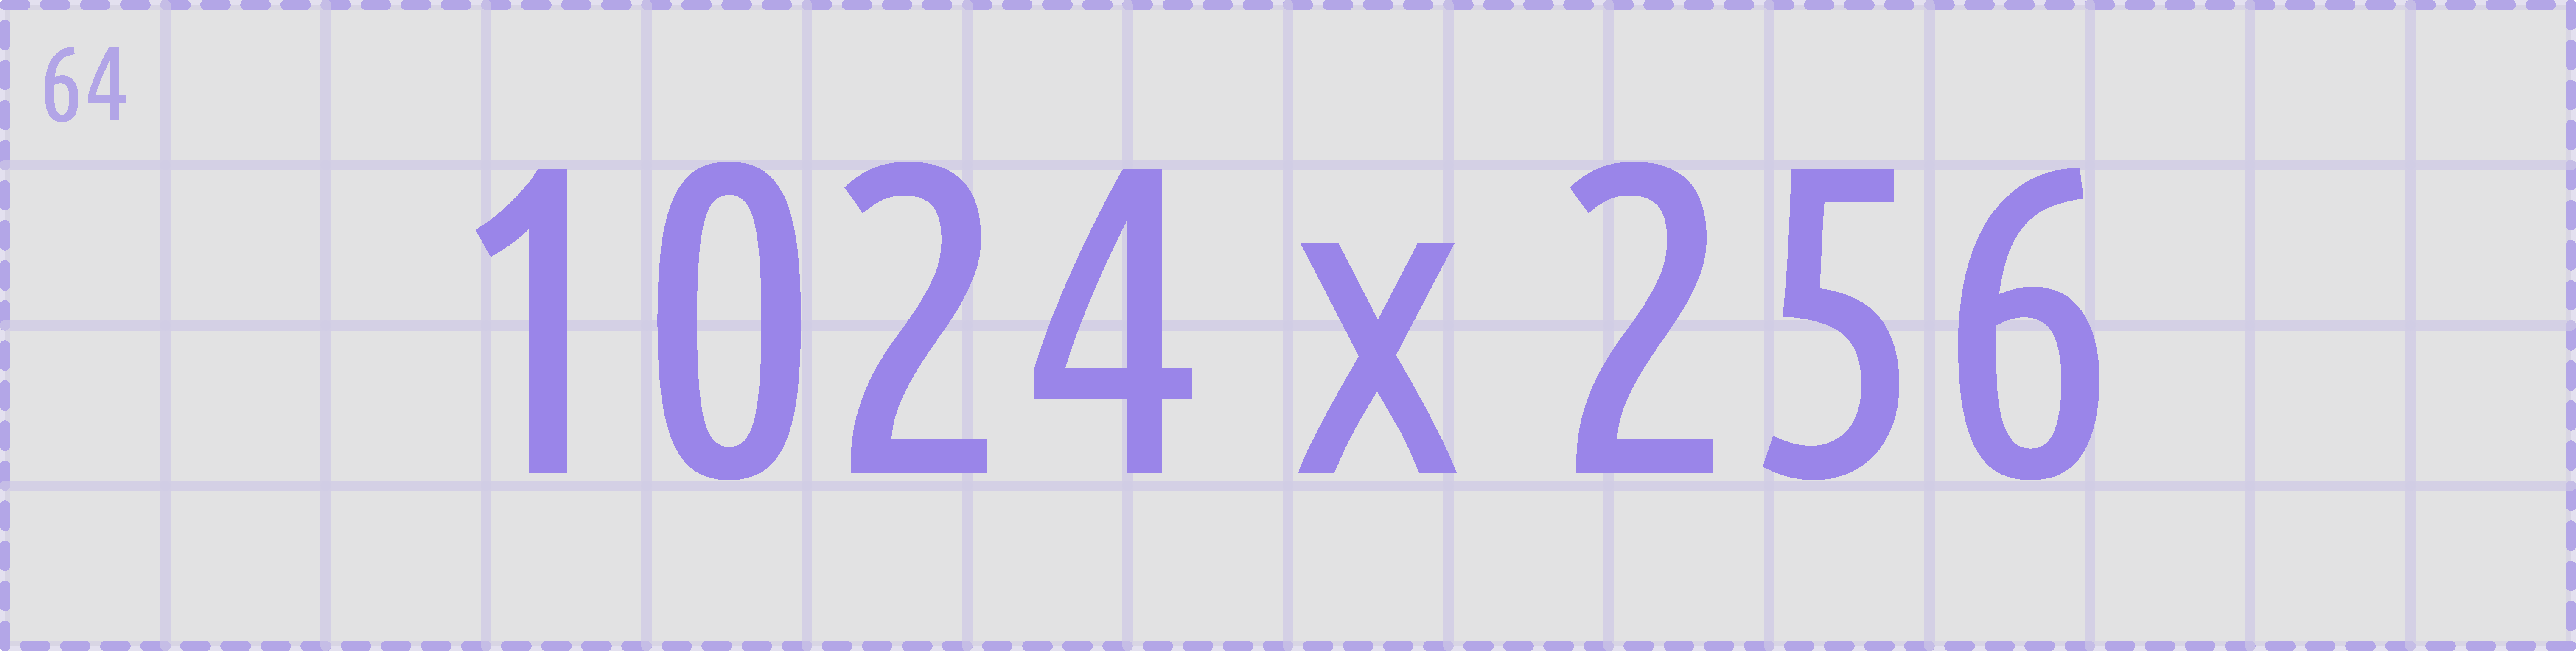
\includegraphics[width = 0.99\textwidth]{fig_1024x256.pdf}
%   \caption{Diagram of the efficient Matrix-Differential solver to compute the unknown Lagrangian entries in the model \eqref{eq:C2:dynamic_model}}
%   \vspace{-0.1cm}
%   \label{fig:C2:EX1:strain_ref}
% \end{figure}
% \begin{figure}[!t]
%  \vspace{-3mm}
%   \centering
%   \def\svgwidth{0.9\linewidth}
%   \input{./3_chapters/2_chapter/img/fig_C2_solver_diagram.pdf_tex}
%   \vspace{-0.25cm}
%   \caption{bla}
%   \vspace{-0.1cm}
%   \label{fig:C2:stiffness_model}
% \end{figure}
%
We wish to stress that $\mat{F}_1$ collects all elements related to the forward kinematics, whereas $\mat{F}_2$ contains the dynamic entities related to the Lagrangian model. Following the spatial Matrix-Differential equation in \eqref{eq:C2:MDE} above, its solution will be a matrix $\mat{Z} := \text{blkdiag}\left( \mat{Z}_1, \mat{Z}_2 \right)$ composed of two state matrices $\mat{Z}_1$ and $\mat{Z}_2$:
%
\begin{align}
\mat{Z}_1(\sigma,\q,\dq) & := \begin{pmatrix}
\begin{matrix}
\PhiB  & \gammaB \\ 0_{3\times3} &  0_{3}
\end{matrix} \;\; \vrule & \!\mat{B}_1 & \vrule & \!\mat{B}_2 \;\;\;
 \end{pmatrix}, \\[0.5em]
\mat{Z}_2(\sigma,\q,\dq) & := \begin{pmatrix} \mat{M} & \mat{C} & \mat{f}\!\grav \end{pmatrix},
\end{align}
%
Such a set of Matrix-Differentials as in \eqref{eq:C2:MDE} are not supported natively by standard ODE solvers. Therefore, an explicit second-order Runge-Kutta solver for MDEs is developed such that efficiently computes the evolution of the state matrix $\mat{Z}$ along $\Xs = [0,L]$. The numerical solver is written in \matlab \texttt{2021a} and it can be found in the public repository of \sorotoki (see implementation at \cite{SorotokiCode}).

As for state trajectories along the temporal regime $\mathbb{T} = [0,T]$, an implicit trapezoidal integration scheme is proposed to solve the approximated continuum dynamics, which are generally less conservative on discretization to preserve numerical stability. Here implicit schemes are favored over the explicit scheme since a coarser time integration can significantly increase real-time performance. In addition, to further boost the performance of the temporal integration, a cost-effective approximation of the Hessian is introduced. For more detail on the temporal integration scheme of the solver can be found in Appendix \ref{app:C2:timeint}


%%%%%%%%%%%%%%%%%%%%%%%%%%%%%%%%%%%%%%%%%%%%%%%%%%%%%%%%%%%%%%%%%%%%%%%%%%%%%%%%


%\part{Control and Sensing Strategies}\label{part: control}
% \cleardoublepage
% \part{Name of second part}\label{part: part2}
% \include{3_chapters/1_introduction/}
% %
% \cleardoublepage
% \part{Conclusions and recommendations}\label{part: closing}
% \chapter{Conclusions and recommendations}
\label{chap: conclusions}
\thispagestyle{empty}

\section{Conclusions}

\lipsum[20-23]
Restate your thesis objective.

\vspace*{3mm}
\objective{State the objective of your PhD research here.}



%**********************************************************************%


\section{Recommendations}

\lipsum[1-4]

%%%% APPENDIX ******************************************************************
\appendix
\cleardoublepage
%\part{Appendices}
\definecolor{thumbcolor}{gray}{0.4}     % Change the color of the thumb index tags to gray
%\chapter{Appendix name}
\label{app: appendix 1}

\section{Section header}

\lipsum[1-4]


%%%% BACK MATTER ***************************************************************
\isstarredchaptertrue           % This state variable is used for creating the thumb index by indicating that the following chapter is not numbered (i.e. \chapter*{})
\bookmarksetup{startatroot}
\addtocontents{toc}{\bigskip}%
%%!TEX root = ../thesis.tex
%\footnotesize
{\fontsize{9pt}{10pt}\selectfont

\bibliographystyle{ieeetr}
%\bibliographystyle{apalike}
\cleardoublepage
\phantomsection
\addcontentsline{toc}{chapter}{\bibname}
\bibliography{5_bibliography/MyBib}
%
}

\normalsize

%\chapter*{Acknowledgments}
\addcontentsline{toc}{chapter}{Acknowledgements}
\markboth{Acknowledgements}{Acknowledgements}
\vspace{-5mm}

% When I was young I always wanted to pursue a scientific career. The pursuit of achieving my doctorate's degree has been by far the largest and heaviest stepping stone in that career. I have been extremely fortune not only in the opportunities that (sometimes seemingly) I've been given but also with the relations that have fruited over the past years.

% It is no secret that without these individuals I'd be unable to reach these achievements in life.

As I embark on the end of my PhD journey, I am somewhat reminded of the Latin motto of the Eindhoven University: ``\textit{Mens agitat molem},'' which translates to ``\textit{Mind moves the mass}.'' This beautiful phrase perhaps encapsulates the essence of my academic pursuit, where other minds played a pivotal role in influencing and reshaping the world around me. Throughout my PhD, I have had the extreme privilege of connecting with various brilliant scholars, mentors, fellow students, and (new) friends who have expanded my understanding within the areas of research, but more importantly, beyond such scopes. ``textit{Mens agitat molem}'' is evident in the collaborative discussions, debates, exchanges of ideas, and connections that have fueled my personal growth and pushed me -- the metaphorical ``mass'' -- forward throughout these years.

First, I would like to express my gratitude to my first promotor. Henk, ik wil je bedanken  voor alle mogelijkheden die je mij hebt geboden tijdens en vooraf mijn promotietraject. Ik heb het gevoel dat onze visie voor het veld 'soft robotics' altijd parallel heeft gelopen, en dit heeft niet alleen geleid tot een uiterst prettige samenwerking, maar heeft mij ook de vrijheid gegeven om mijzelf als onderzoeker vrij te ontwikkelen. Je scherpe opmerkingen, maar vooral ook je humoristische inbreng, werden zeer gewaardeerd. Je begeleiding, steun, en expertise hebben mij geholpen om mijn promotietraject tot een succesvol einde te brengen. Bedankt voor alles.

Secondly, I would like to express my sincere appreciation to my co-promoter, Sasha. I am immensely grateful for your unwavering support and open-mindedness throughout the years, but above all, for your remarkable patience with me. You have consistently provided me with the freedom to explore new ideas, and we have engaged in numerous captivating discussions connected to the realm of soft robotics. Furthermore, I deeply value the time and availability you have dedicated to me, even without prior notice. This has truly made me feel that your doors are always open – a practice that I have come to embrace with my own students over the course of my Ph.D. career.

My sincere gratitude also goes to the committee members who have been part of reviewing the thesis and participating in the public defense: Jaap den Toonder, Gijs Krijnen, Bas Overvelde, and Anibal Ollero; and my gratitude to Patrick Anderson who agreed to chair the defense ceremony.

I would also like to express my gratitude to the members of the {Wearable Robotics} project. Herman, thank you for assembling such a wonderful and diverse group of researchers. The monthly telecoms and yearly consortia that brought us together were inspirational and insightful, and I thoroughly enjoyed the platform that was given for discussions and collaboration. Ali, thank you for all the fruitful collaboration, and I am proud of our collaboration and publication, which has become a chapter of your dissertation. What an honor to be part of your doctoral work! Mariska, thank you for all your interesting input and the opportunities you have given Ali and me to gain insight into the clinical world. I also want to thank the other fantastic researchers from Twente: Martijn, Cristina, Alejandro, Ander, Michelle, and the folks from Delft, Cor, and Wouter; you guys are truly inspiring engineers.

I am deeply grateful to my wonderful ex-colleagues with whom I have had the pleasure of working on various courses: Astrid, Bayu, Carlos, Ines, Nathan, Matt, and Ruben, and a few others I'd like to mention separately. Alessandro, I want to express my heartfelt appreciation for our collaboration on the robotics course. Your consistent interest in my project and the occasional interesting emails on related research topics have been truly valuable. Irene, bedankt voor onze vlekkeloze samenwerking tijdens de Haptics en voor het verwelkomen in jullie onderzoeksgroep en lab. Rob, ik heb oprecht genoten van onze samenwerking bij Dynamics, maar wat ik het meest bewonder, is jouw standvastige aanwezigheid tijdens de ``Vrijmibo'', zowel in persoon als virtueel. Gerard, bedankt voor de boeiende discussies die we hebben gehad onder het genot van een kopje koffie. Ik wil ook graag Harry, Peter (2x) erkennen voor hun lab ondersteuning. Tot slot, Geertje, hartelijk dank voor alles wat je hebt gedaan. De zorg die je hebt voor onze groep, maar ook voor elk individu, blijft niet onopgemerkt. Jij bent werkelijk de steunpilaar van onze groep. Thank you all for making my time at the TU/e memorable and rewarding.

To the students I had the pleasure of supervising: Erwin, Sef, Willem, Has, and Yoshi, and a few others I'd like to mention separately. Benn, I feel extremely lucky that, out of all the students who rejected my B.Sc project proposal, you were the one to give it a shot. Call it fate. I was thrilled to hear you had joined our group, and I now know the ``Vrijmibo'' is in good hands. Hoang, it was a pleasure supervising you. Thanks for the ergonomic mouse which I am still using while finishing up these last pages. Also, Tijn, thanks for the extremely nice collaboration. It was a pleasure reading all of your ``extensive'' reports, and I was surprised by your kind words in the acknowledgements of your thesis.

I would also like to express my heartfelt gratitude to my former office mates. Tom, ik ben dankbaar voor de begeleiding en steun die je hebt geboden tijdens de begindagen als jonge promovendus. Ook onze samenwerkingen op jouw CAD-gerelateerde projecten voor de fiets waren echt vermakelijk. Rinus, bedankt voor jouw luisterend oor en betrokkenheid bij allerlei interessante discussies op kantoor. Ik zal onze uitgebreide whiteboard discussies missen, die immers essentieel zijn geweest voor de vormgeving van deze scriptie. Jouw aanwezigheid als kantoorgenoot is waardevol geweest, vooral wanneer ik een extra `\emph{mind}' nodig had om mentale blokkades te verhelpen. Ana, I will cherish the memories of our delightful coffee breaks and the engaging discussions we had, particularly the ones we shared digitally from my kitchens during the pandemic. I am also grateful for the opportunity to publish together. Lastly, I would like to acknowledge Guo and Nishant, albeit our time together in the office was brief, your contributions and camaraderie were greatly appreciated. 

Also thanks to all my fellow Ph.D.s who've I had to pleasure to share the occasional coffee. Thanks to my other coworkers from D\&C: Alexander, Andy, Bas, Dirk, Dipankar, Fahim, Haleh, Jizheng, Joey, Kaidong, Kevin, Lars (2x), Luuk (2x), Maarten, Philipp, Rapha\"{e}l, Raul, Roeland, Rigo, Sebastiaan, Semih, Viral, Wouter (2x), and Yuzhe; and the folks from CST: Bardia, Casper, Hao, Jilles, Koen (2x), Leontine, Maurice, Max, Nard, Noud, Paul, Puck, Roy, Sven, and Tomas. Also thanks to all the older former colleagues that have improved the Ph.D. experience significantly: Alex, Chyannie, Daniel (2x), Frans, Igor, Kirill, Lennart, Leroy, Michiel, Quentin, Robert, Rishi, Ruud, Sajad, Suraj, and Veronica.

There are a few colleagues I'd like to mention separately. Krishna, your unbreakable optimism and your laugh that echoes through the halls of Gemini-South are seriously infectious and uplifting. Thanks for all that you have organized. Dario and Alessia, thanks for all the nice Italian coffee and cookies -- grazie mille! Jari, hartelijk dank dat je me feitelijk gratis hebt meegenomen naar Rammstein. Het was een mooie gelegenheid waarop mijn ``lange-haar-fase'' zijn vruchten heeft afgeworpen. Ruud, hartelijk dank voor je sporadische bezoeken aan mijn kantoor, je aansporing om die ene keer naar de sportschool te gaan en al onze interessante filosofische discussies. Ricky, het was altijd een genoegen wanneer je langs kwam op kantoor. Mischa, it was a pleasure being my partner-in-crime when infiltrating the Benelux meeting. It was a legendary evening, by far the best Benelux meeting for me! Naturally, I have to extend my gratitude to Venkata for not showing up, so I could borrow his name tag, and all the other PhDs who heroically gifted all their beers to me. Femke and Mahboubeh, thank you for the fruitful collaborations. I was thrilled to see more people starting to work on soft robotics within our group, and I am delighted that we had the opportunity to publish together. A small shoutout to the people at AMOLF: Alberto, Mannus, Paul, Sergio, and (the legendary) Shibo; for a memorable experience at last year's Dutch Soft Robotics Symposium in Twente.
The same naturally applies to the folks of the Reshape group. Also special thanks to those that celebrated my hand-in date, those that pleasantly surprised me on my 30\textsuperscript{th} birthday, and the regulars at the ``\textit{VrijMiBo}''. To all of you, my heartfelt thanks for transforming my time at the University into an unforgettable, rewarding experience full of cherished friendships.

Camiel, ook bedankt voor al die vroege ochtendtreinritten. De mogelijkheid om alles aan jou voor te leggen hebben mij veel mentale rust gegeven en hebben deelsgeleid tot het succesvol afronden van dit boekje. Falco, bedankt voor je constante interesse, suggesties voor zelfverbeteringsboeken, game- en pizzanachten. Roos, bedankt voor je steun en levensadvies. Jullie zijn geweldige vrienden geweest gedurende al die jaren, een echte vangst! Martijn en Bob, bedankt voor alle whiskey-(maar voornamelijk speciaal bier)-avonden. Dank aan Anne en Britt voor alle ``gamy-gamy'' avonden, filmavonden, tripjes Groningen, en natuurlijk onze magische reis naar Londen -- kan niet wachten op een vervolg (of trilogie). Jullie vriendschap is essentieel motivatievoer geweest voor dit boekje. Gijs en Bob, bedankt voor het accepteren van de rol van paranymph, met twee van mijn oudste vrienden aan mijn zijde heeft de tegenpartij geen kans. Mijn dankbaarheid strekt zich natuurlijk ook uit naar de andere oldies Roel, Michel, en ook Panda. Xavier, bedankt voor al je frequente herinneringen om af te spreken. Dank aan Dominique voor het organiseren van al deze geweldige reizen en avonturen die we de afgelopen plus-tien jaar hebben gehad, grotendeels dankzij jouw fantastische organisatietalent. De recente Ardennen en Londen trip waren de hoognodige pauzes waar ik zo naar verlangde tijdens mijn promotieonderzoek. Ties, bedankt dat je altijd mijn vaste aanspreekpunt bent geweest voor alles wat met concerten te maken heeft. En vanzelfsprekend gaat mijn dank ook uit naar de andere old-timers: Cynthia, Siem, Jeffrey, Etienne, Jolijn en Dennis. Diem en Lissane, bedankt voor alle gezelligheid en de geweldige Foals LP die jullie hebben geschonken - mijn favoriet tot heden.

Manu und Nina, vielen Dank f\"{u}r eure Gastfreundschaft in R\"{o}dern, die Biere und das fantastische deutsche Essen, die speziellen, thematischen Geburtstagspartys - nat\"{u}rlich war Big Lewboski meine Lieblingsparty - und die Brettspielabende. Johannes, vielen Dank f\"{u}r dein wissenschaftliches Interesse, und Sarah, danke f\"{u}r deinen herzlichen Empfang in die Familie. Regina und Karsten, danke, dass ihr mich so in eure Familie einbezogen habt, so dass ich mich dazugeh\"{o}rig gef\"{u}hlt habe.

Mam, ik wil je enorm bedanken voor al je ongelofelijke support in zowel mijn persoonlijke ontwikkeling als mijn carrière. Jouw constante aanmoediging en steun vanaf het begin hebben eindelijk hun vruchten afgeworpen. Ik ben enorm dankbaar en trots dat ik jou als mijn moeder heb. Ook wil ik graag mijn broer, Myron of Madji, bedanken. De steun die jullie hebben aangeboden is ongelofelijk waardevol en heeft geleid tot het stand komen van deze thesis. Zonder jullie zou ik dit nooit hebben kunnen bereiken. Pap, bedankt voor je interesse en steun gedurende de afgelopen jaren. Jouw betrokkenheid heeft me altijd gemotiveerd en ge\"{i}nspireerd om het beste uit mezelf te halen. Ook Rachel verdient een speciale dankjewel, je betrokkenheid in onze familie is goud waard.

Also, thanks to those few I might have forgotten to mention. I have an exceptionally bad memory for names, but I won't easily forget a face.

Last but not least, my dearest Miriam, words cannot express the joy I have felt having you by my side during these ``\textit{tough}'' albeit ``\textit{adventurous}'' times. You were the light that has guided my soul to a safe and happy haven, and without you, I was probably not able to make it.

\begin{flushright}
Brandon Caasenbrood \\
Eindhoven, September 2023
\end{flushright}  
%!TEX root = ../thesis.tex
%*********************************************************************************%
\chapter*{List of publications}
\addcontentsline{toc}{chapter}{List of publications}
\markboth{List of publications}{List of publications}
\newcommand{\ipj}{(\textit{in preparation for journal submission})}
\newcommand{\cur}{(\textit{under review})}
\newcommand{\sbm}{(\textit{submitted})}
\newcommand{\acp}{(\textit{accepted})}
\newcommand{\inp}{(\textit{in press})}

% \section*{Preliminary titles}
% \begin{enumerate}[leftmargin=2.5mm]
% \item A Control-oriented Perspective on Design and Modeling of Soft Robotic Systems;
% \item Towards a Unified Framework for Design and Model-based Control of Soft Robots;
% \item Addressing the Open Challenges in Soft Robotics: from Design to Model-based Control
% \item Design and Control Strategies for Soft Robotic Systems;
% \item Design, Modeling, Simulation and Control of Soft Robots.
% \item Design, Modeling and Control Strategies for Soft Robotics Systems;
% \item (Soft Manipulators/Soft Robotic Manipulators?)
% \end{enumerate}
%
% \section*{Preliminary committee members}
% \begin{itemize}[leftmargin=4mm]
% \item prof. J. den Toonder (TU/e, Microsystems, ICMS) \vspace{-2mm}
% \item dr. R. Luttge (TU/e, Microsystems) - Backup for Jaap \\ ............................................................................................... \vspace{-2mm}
% \item prof. G. Krijnen (Twente University) Technologies) \vspace{-2mm}
% \item prof. C.C.L. Wang (Delft University) \vspace{-2mm} \href{https://ieeexplore.ieee.org/document/9426391}{[1]}, \href{https://www.researchgate.net/publication/347965436_Jacobian-based_learning_for_inverse_kinematics_of_soft_robots}{[2]}
% \item prof R. Carloni (Rijksuniversiteit
% Groningen) - backup for Gijs \\ ............................................................................................... \vspace{-2mm}
% \item dr. E. Franco (Enrico, Imperial College London) \vspace{-2mm} \href{https://link.springer.com/article/10.1007/s11071-021-06817-1}{[1]}, \href{https://ieeexplore.ieee.org/document/9638969}{[2]}
% \item prof. H. Mochiyama (University of Tsukuba) \href{https://www.sciencedirect.com/science/article/pii/S2405896320328226?via%3Dihub}{[1]}, \href{https://ieeexplore.ieee.org/document/1242160}{[2]} \vspace{-2mm}
% \item dr. C. Duriez (INRIA Lille) \href{https://hal.inria.fr/hal-01370347/document}{[1]},\href{https://hal.archives-ouvertes.fr/hal-03192168/document}{[2]}\vspace{-2mm}
% \item prof. R. Katzschmann (ETH Zurich) \href{https://www.liebertpub.com/doi/pdfplus/10.1089/soro.2014.0022}{[1]},\href{https://arpi.unipi.it/retrieve/handle/11568/996018/683882/Final%20manuscript%20IEEE.pdf}{[2]}\vspace{-2mm}
% \item dr. S. Grazioso (University of Naples) \href{https://pubmed.ncbi.nlm.nih.gov/30481112/}{[1]} \vspace{-2mm}
% \item dr. M. Bächer (ETH Zurich) \href{https://pubmed.ncbi.nlm.nih.gov/31891526/}{[1]},\href{https://ieeexplore.ieee.org/document/9312179}{[2]}
% \item Antonio Bicchi - Italian
% \item Annibal Olero - Spain
% \item Bas Overvelde??
% \end{itemize}
\vspace{-10mm}
%*********************************************************************************%
\section*{Peer-reviewed journal articles}
\begin{itemize}[leftmargin=4mm]
  \item B. Caasenbrood, A. Pogromsky and H. Nijmeijer, “\textit{Generative Design of Soft Robotic Actuators -- a Gradient-based Approach}”, Frontiers in Robotics and AI, 2022. \ipj;
\item B. Caasenbrood, A. Pogromsky and H. Nijmeijer, “\textit{Reduced-order Cosserat Models for Soft Robotic
 Systems using FEM-driven Shape Reconstruction}”, Robotics and Automation Letters, 2022. \ipj;
%\item B. Caasenbrood, A. Amoozandeh Nobaveh, M. Janssen, A. Pogromsky, J. Herder, and H. Nijmeijer “\textit{An Energy-efficient Gravity-balancing Wrist Exoskeleton by exploring Compliant Beams and Soft Robotic Actuation},” Wearable Technologies. \ipj;
\item A. Amiri, B. Caasenbrood, D. Liu, N. van de Wouw, and I. Lopez Arteaga, "\textit{An Electric Circuit Model for the Nonlinear Dynamics of Electro-active Liquid Crystal Coatings}", Applied Physics Letters, 2022. \sbm;
\item  B. Caasenbrood, A. Pogromsky and H. Nijmeijer, “\textit{Energy-shaping Controllers for Soft Robot Manipulators through Port-Hamiltonian Cosserat Models}”, SN Computer Science Springer, 2022. \acp;
\item B. Caasenbrood, A. Pogromsky and H. Nijmeijer, "\textit{Control-oriented Models for Hyper-elastic Soft Robots through Differential Geometry of Curves}”, Soft Robotics, 2022.
\end{itemize}

%*********************************************************************************%
\section*{Peer-reviewed articles in conference proceedings}
\begin{itemize}[leftmargin=4mm]
\item B. Caasenbrood, F.E. van Beek, H. Khanh Chu, and I.A. Kuling, “\textit{A Desktop-sized Platform for Real-time Control Applications of Pneumatic Soft Robots},” IEEE International Conference on Soft Robotics, RoboSoft 2022, pp 217-223.
\item A. Amoozandeh Nobaveh, and B. Caasenbrood, "\textit{Design Feasibility of an Energy-efficient Wrist Exoskeleton
using Compliant Beams and Soft Actuators}", Proceedings of the 18th International  Consortium for Rehabilitation Robotics, 2022 (accepted).
\item B. Caasenbrood, A. Pogromsky and H. Nijmeijer, "\textit{Energy-based control for Soft Robots using Cosserat-beam models}”, Proceedings of the 18th International Conference on Informatics in Control, Automation and Robotics, 2021, pp. 311–319.
\item B. Caasenbrood, A. Pogromsky and H. Nijmeijer, "\textit{A Computational Design Framework for Pressure-driven Soft Robots through Nonlinear Topology Optimization}," 2020 3rd IEEE International Conference on Soft Robotics, 2020, pp. 633-638.
\item B. Caasenbrood, A. Pogromsky and H. Nijmeijer, “\textit{Dynamic modeling of hyper-elastic soft robots using spatial curves},” IFAC World Congress, IFAC-PapersOnLine, 2020, pp. 9238-9243.
\end{itemize}

\section*{Invited Talks and non peer-reviewed abstracts}
\begin{itemize}[leftmargin=4mm]
\item B. Caasenbrood, talk on  “\textit{3D-printed Soft Robotics},” Symposium on Robotic Technologies, Ultimaker, 2022. (invited speaker).
\item B. Caasenbrood, \texttt{SOROTOKI}: \textit{an open-source MATLAB toolkit for Design, Modelling and Control of Soft Robots},”   4TU Federation`s Symposium on Soft Robotics, Delft University, 2022. (invited speaker).
\item B. Caasenbrood, “\texttt{SOROTOKI}\textit{: an Open-source Toolkit for Soft Robotics written in MATLAB},”  IEEE International Conference on Soft Robotics, RoboSoft 2022, Edinbrugh. (poster presentation). \texttt{Best Poster Award}
\item B. Caasenbrood, C. Della Santina, and A. Pogromsky, “\textit{Workshop on Model-based Control of Soft Robots},” European Control Conference (ECC), 2021. (main organizer).
\item B. Caasenbrood, talk on  “\textit{Towards Design and Control of Soft Robotics},” 4TU Symposium on Soft Robotics (digital), 2020. (invited speaker).
\item B. Caasenbrood, talk on  “\textit{3D-printed Soft Robotics},” Symposium on Robotic Technologies, 2019. (invited speaker).
\item B. Caasenbrood, A. Pogromsky and H. Nijmeijer, talk on  “\textit{Forward Dynamics of Hyper-elastic Soft Robotics},” 39th Benelux Meeting on Systems and Control, 2019. (abstract).
\item B. Caasenbrood, A. Pogromsky and H. Nijmeijer, talk on  “\textit{Dynamical modeling and control of continuum soft robots},” 37th Benelux Meeting on Systems and Control, 2018. (abstract).
\end{itemize}

%%*********************************************************************************%
\chapter*{Curriculum Vitae}
\addcontentsline{toc}{chapter}{Curriculum Vitae}
\markboth{Curriculum Vitae}{Curriculum Vitae}




%\newpage {~}
\thispagestyle{empty}

\ifprint{}
\else
\newpage {~}
\thispagestyle{empty}
\fi

%%%% BACK **********************************************************************
%\cover{thesis_back.pdf}    % Adds your thesis' back cover if the option 'print' is NOT used. Printing companies require the thesis cover to be supplied separately and in a different format. Definition of \cover{} is given in commands.tex.

\end{document}
%%%% THAT's ALL FOLKS **********************************************************
